\chapter{Three Processors}
\label{chap:p3}

\section{Some proofs that HLF is not optimal for P3}

This section showcases some situations, where HLF is not optimal. Figure \ref{fig:hlf-001112} an intree, where HLF can choose at some points, and different choices result in different runtimes. 

Figures \ref{fig:hlf-vs-opt-0012346688}, \ref{fig:hlf-vs-opt-0012446788} and \ref{fig:hlf-vs-opt-00123455799} show two examples that prove that HLF is not optimal for three processors.

\begin{figure}[ht]
  \centering
  \renewcommand{\leveltopI}{-15cm + \leveltop}
\renewcommand{\leveltopII}{-15cm + \leveltopI}
\renewcommand{\leveltopIII}{-15cm + \leveltopII}
\renewcommand{\leveltopIIII}{-15cm + \leveltopIII}
\renewcommand{\leveltopIIIII}{-15cm + \leveltopIIII}
\renewcommand{\leveltopIIIIII}{-15cm + \leveltopIIIII}
\renewcommand{\leveltopIIIIIII}{-15cm + \leveltopIIIIII}
\begin{tikzpicture}[scale=.2, anchor=south]
\begin{scope}[yshift=\leveltopI cm]
\matrix (line1)[column sep=0.5cm] {
\node[draw=black, rectangle split,  rectangle split parts=4] (sn0x8968ef8){
\footnotesize{100}
\nodepart{two}
\begin{tikzpicture}[scale=.2]
\node[circle, scale=0.75, fill] (tid0) at (3,1.5){};
\node[circle, scale=0.75, fill] (tid1) at (2.25,3){};
\node[circle, scale=0.75, fill, red] (tid3) at (0.75,4.5){};
\node[circle, scale=0.75, fill, red] (tid4) at (2.25,4.5){};
\node[circle, scale=0.75, fill, red] (tid5) at (3.75,4.5){};
\draw[](tid1) -- (tid3);
\draw[](tid1) -- (tid4);
\draw[](tid1) -- (tid5);
\node[circle, scale=0.75, fill] (tid2) at (5.25,3){};
\node[circle, scale=0.75, fill] (tid6) at (5.25,4.5){};
\draw[](tid2) -- (tid6);
\draw[](tid0) -- (tid1);
\draw[](tid0) -- (tid2);
\end{tikzpicture}
\nodepart{three}
\footnotesize{4.38889}
\nodepart{four}
\footnotesize{$1$}
};
 & 
\\
};
\end{scope}
\begin{scope}[yshift=\leveltopII cm]
\matrix (line2)[column sep=0.5cm] {
\node[draw=black, rectangle split,  rectangle split parts=4] (sn0x8969f98){
\footnotesize{100}
\nodepart{two}
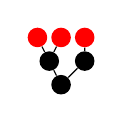
\begin{tikzpicture}[scale=.2]
\node[circle, scale=0.75, fill] (tid0) at (2.25,1.5){};
\node[circle, scale=0.75, fill] (tid1) at (1.5,3){};
\node[circle, scale=0.75, fill, red] (tid3) at (0.75,4.5){};
\node[circle, scale=0.75, fill, red] (tid4) at (2.25,4.5){};
\draw[](tid1) -- (tid3);
\draw[](tid1) -- (tid4);
\node[circle, scale=0.75, fill] (tid2) at (3.75,3){};
\node[circle, scale=0.75, fill, red] (tid5) at (3.75,4.5){};
\draw[](tid2) -- (tid5);
\draw[](tid0) -- (tid1);
\draw[](tid0) -- (tid2);
\end{tikzpicture}
\nodepart{three}
\footnotesize{4.05556}
\nodepart{four}
\footnotesize{$67\:33$}
};
 & 
\\
};
\end{scope}
\begin{scope}[yshift=\leveltopIII cm]
\matrix (line3)[column sep=0.5cm] {
\node[draw=black, rectangle split,  rectangle split parts=4] (sn0x8969bb0){
\footnotesize{66.6667}
\nodepart{two}
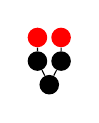
\begin{tikzpicture}[scale=.2]
\node[circle, scale=0.75, fill] (tid0) at (1.5,1.5){};
\node[circle, scale=0.75, fill] (tid1) at (0.75,3){};
\node[circle, scale=0.75, fill, red] (tid3) at (0.75,4.5){};
\draw[](tid1) -- (tid3);
\node[circle, scale=0.75, fill] (tid2) at (2.25,3){};
\node[circle, scale=0.75, fill, red] (tid4) at (2.25,4.5){};
\draw[](tid2) -- (tid4);
\draw[](tid0) -- (tid1);
\draw[](tid0) -- (tid2);
\end{tikzpicture}
\nodepart{three}
\footnotesize{3.75}
\nodepart{four}
\footnotesize{$1$}
};
 & 
\node[draw=black, rectangle split,  rectangle split parts=4] (sn0x896a3b8){
\footnotesize{33.3333}
\nodepart{two}
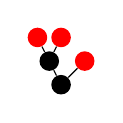
\begin{tikzpicture}[scale=.2]
\node[circle, scale=0.75, fill] (tid0) at (2.25,1.5){};
\node[circle, scale=0.75, fill] (tid1) at (1.5,3){};
\node[circle, scale=0.75, fill, red] (tid3) at (0.75,4.5){};
\node[circle, scale=0.75, fill, red] (tid4) at (2.25,4.5){};
\draw[](tid1) -- (tid3);
\draw[](tid1) -- (tid4);
\node[circle, scale=0.75, fill, red] (tid2) at (3.75,3){};
\draw[](tid0) -- (tid1);
\draw[](tid0) -- (tid2);
\end{tikzpicture}
\nodepart{three}
\footnotesize{3.66667}
\nodepart{four}
\footnotesize{$67\:33$}
};
 & 
\\
};
\end{scope}
\draw (sn0x8968ef8.south) -- (sn0x8969f98.north);
\draw (sn0x8969f98.south) -- (sn0x8969bb0.north);
\draw (sn0x8969f98.south) -- (sn0x896a3b8.north);
\end{tikzpicture}
\renewcommand{\leveltopI}{-15cm + \leveltop}
\renewcommand{\leveltopII}{-15cm + \leveltopI}
\renewcommand{\leveltopIII}{-15cm + \leveltopII}
\renewcommand{\leveltopIIII}{-15cm + \leveltopIII}
\renewcommand{\leveltopIIIII}{-15cm + \leveltopIIII}
\renewcommand{\leveltopIIIIII}{-15cm + \leveltopIIIII}
\renewcommand{\leveltopIIIIIII}{-15cm + \leveltopIIIIII}
\begin{tikzpicture}[scale=.2, anchor=south]
\begin{scope}[yshift=\leveltopI cm]
\matrix (line1)[column sep=0.5cm] {
\node[draw=black, rectangle split,  rectangle split parts=4] (sn0x8969e68){
\footnotesize{100}
\nodepart{two}
\begin{tikzpicture}[scale=.2]
\node[circle, scale=0.75, fill] (tid0) at (3,1.5){};
\node[circle, scale=0.75, fill] (tid1) at (2.25,3){};
\node[circle, scale=0.75, fill, red] (tid3) at (0.75,4.5){};
\node[circle, scale=0.75, fill, red] (tid4) at (2.25,4.5){};
\node[circle, scale=0.75, fill] (tid5) at (3.75,4.5){};
\draw[](tid1) -- (tid3);
\draw[](tid1) -- (tid4);
\draw[](tid1) -- (tid5);
\node[circle, scale=0.75, fill] (tid2) at (5.25,3){};
\node[circle, scale=0.75, fill, red] (tid6) at (5.25,4.5){};
\draw[](tid2) -- (tid6);
\draw[](tid0) -- (tid1);
\draw[](tid0) -- (tid2);
\end{tikzpicture}
\nodepart{three}
\footnotesize{4.37037}
\nodepart{four}
\footnotesize{$67\:33$}
};
 & 
\\
};
\end{scope}
\begin{scope}[yshift=\leveltopII cm]
\matrix (line2)[column sep=0.5cm] {
\node[draw=black, rectangle split,  rectangle split parts=4] (sn0x8969f98){
\footnotesize{66.6667}
\nodepart{two}
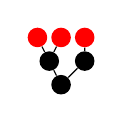
\begin{tikzpicture}[scale=.2]
\node[circle, scale=0.75, fill] (tid0) at (2.25,1.5){};
\node[circle, scale=0.75, fill] (tid1) at (1.5,3){};
\node[circle, scale=0.75, fill, red] (tid3) at (0.75,4.5){};
\node[circle, scale=0.75, fill, red] (tid4) at (2.25,4.5){};
\draw[](tid1) -- (tid3);
\draw[](tid1) -- (tid4);
\node[circle, scale=0.75, fill] (tid2) at (3.75,3){};
\node[circle, scale=0.75, fill, red] (tid5) at (3.75,4.5){};
\draw[](tid2) -- (tid5);
\draw[](tid0) -- (tid1);
\draw[](tid0) -- (tid2);
\end{tikzpicture}
\nodepart{three}
\footnotesize{4.05556}
\nodepart{four}
\footnotesize{$67\:33$}
};
 & 
\node[draw=black, rectangle split,  rectangle split parts=4] (sn0x896a940){
\footnotesize{33.3333}
\nodepart{two}
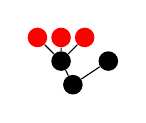
\begin{tikzpicture}[scale=.2]
\node[circle, scale=0.75, fill] (tid0) at (3,1.5){};
\node[circle, scale=0.75, fill] (tid1) at (2.25,3){};
\node[circle, scale=0.75, fill, red] (tid3) at (0.75,4.5){};
\node[circle, scale=0.75, fill, red] (tid4) at (2.25,4.5){};
\node[circle, scale=0.75, fill, red] (tid5) at (3.75,4.5){};
\draw[](tid1) -- (tid3);
\draw[](tid1) -- (tid4);
\draw[](tid1) -- (tid5);
\node[circle, scale=0.75, fill] (tid2) at (5.25,3){};
\draw[](tid0) -- (tid1);
\draw[](tid0) -- (tid2);
\end{tikzpicture}
\nodepart{three}
\footnotesize{4}
\nodepart{four}
\footnotesize{$1$}
};
 & 
\\
};
\end{scope}
\begin{scope}[yshift=\leveltopIII cm]
\matrix (line3)[column sep=0.5cm] {
\node[draw=black, rectangle split,  rectangle split parts=4] (sn0x8969bb0){
\footnotesize{44.4444}
\nodepart{two}
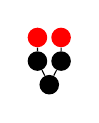
\begin{tikzpicture}[scale=.2]
\node[circle, scale=0.75, fill] (tid0) at (1.5,1.5){};
\node[circle, scale=0.75, fill] (tid1) at (0.75,3){};
\node[circle, scale=0.75, fill, red] (tid3) at (0.75,4.5){};
\draw[](tid1) -- (tid3);
\node[circle, scale=0.75, fill] (tid2) at (2.25,3){};
\node[circle, scale=0.75, fill, red] (tid4) at (2.25,4.5){};
\draw[](tid2) -- (tid4);
\draw[](tid0) -- (tid1);
\draw[](tid0) -- (tid2);
\end{tikzpicture}
\nodepart{three}
\footnotesize{3.75}
\nodepart{four}
\footnotesize{$1$}
};
 & 
\node[draw=black, rectangle split,  rectangle split parts=4] (sn0x896a3b8){
\footnotesize{55.5556}
\nodepart{two}
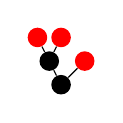
\begin{tikzpicture}[scale=.2]
\node[circle, scale=0.75, fill] (tid0) at (2.25,1.5){};
\node[circle, scale=0.75, fill] (tid1) at (1.5,3){};
\node[circle, scale=0.75, fill, red] (tid3) at (0.75,4.5){};
\node[circle, scale=0.75, fill, red] (tid4) at (2.25,4.5){};
\draw[](tid1) -- (tid3);
\draw[](tid1) -- (tid4);
\node[circle, scale=0.75, fill, red] (tid2) at (3.75,3){};
\draw[](tid0) -- (tid1);
\draw[](tid0) -- (tid2);
\end{tikzpicture}
\nodepart{three}
\footnotesize{3.66667}
\nodepart{four}
\footnotesize{$67\:33$}
};
 & 
\\
};
\end{scope}
\draw (sn0x8969e68.south) -- (sn0x8969f98.north);
\draw (sn0x8969e68.south) -- (sn0x896a940.north);
\draw (sn0x8969f98.south) -- (sn0x8969bb0.north);
\draw (sn0x8969f98.south) -- (sn0x896a3b8.north);
\draw (sn0x896a940.south) -- (sn0x896a3b8.north);
\end{tikzpicture}
%%% Local Variables:
%%% TeX-master: "thesis/thesis.tex"
%%% End: 
  \caption{HLF on 001112. Different runs of HLF do not necessarily produce the same result.}
  \label{fig:hlf-001112}
\end{figure}

\begin{figure}[ht]
  \centering
  \renewcommand{\leveltopI}{-15cm + \leveltop}
\renewcommand{\leveltopII}{-15cm + \leveltopI}
\renewcommand{\leveltopIII}{-15cm + \leveltopII}
\renewcommand{\leveltopIIII}{-15cm + \leveltopIII}
\renewcommand{\leveltopIIIII}{-15cm + \leveltopIIII}
\renewcommand{\leveltopIIIIII}{-15cm + \leveltopIIIII}
\renewcommand{\leveltopIIIIIII}{-15cm + \leveltopIIIIII}
\renewcommand{\leveltopIIIIIIII}{-15cm + \leveltopIIIIIII}
\renewcommand{\leveltopIIIIIIIII}{-15cm + \leveltopIIIIIIII}
\renewcommand{\leveltopIIIIIIIIII}{-15cm + \leveltopIIIIIIIII}
\renewcommand{\leveltopIIIIIIIIIII}{-15cm + \leveltopIIIIIIIIII}
\begin{tikzpicture}[scale=.2, anchor=south]
\begin{scope}[yshift=\leveltopI cm]
\matrix (line1) [column sep=1cm] {
\node[draw=black, rectangle split,  rectangle split parts=3] (sn0x14639f0){
\begin{tikzpicture}[scale=.2]
\node[circle, scale=0.75, fill] (tid0) at (3,1.5){};
\node[circle, scale=0.75, fill] (tid1) at (2.25,3){};
\node[circle, scale=0.75, fill] (tid3) at (2.25,4.5){};
\node[circle, scale=0.75, fill] (tid5) at (2.25,6){};
\node[circle, scale=0.75, fill] (tid7) at (1.5,7.5){};
\node[circle, scale=0.75, fill, red] (tid9) at (0.75,9){};
\node[circle, scale=0.75, fill, red] (tid10) at (2.25,9){};
\draw[](tid7) -- (tid9);
\draw[](tid7) -- (tid10);
\node[circle, scale=0.75, fill, red] (tid8) at (3.75,7.5){};
\draw[](tid5) -- (tid7);
\draw[](tid5) -- (tid8);
\draw[](tid3) -- (tid5);
\draw[](tid1) -- (tid3);
\node[circle, scale=0.75, fill] (tid2) at (5.25,3){};
\node[circle, scale=0.75, fill] (tid4) at (5.25,4.5){};
\node[circle, scale=0.75, fill] (tid6) at (5.25,6){};
\draw[](tid4) -- (tid6);
\draw[](tid2) -- (tid4);
\draw[](tid0) -- (tid1);
\draw[](tid0) -- (tid2);
\end{tikzpicture}
\nodepart{two}
\footnotesize{6.96798}
\nodepart{three}
\footnotesize{$33\:67$}
};
 & 
\\
};
\end{scope}
\begin{scope}[yshift=\leveltopII cm]
\matrix (line2) [column sep=1cm] {
\node[draw=black, rectangle split,  rectangle split parts=3] (sn0x1460d30){
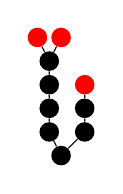
\begin{tikzpicture}[scale=.2]
\node[circle, scale=0.75, fill] (tid0) at (2.25,1.5){};
\node[circle, scale=0.75, fill] (tid1) at (1.5,3){};
\node[circle, scale=0.75, fill] (tid3) at (1.5,4.5){};
\node[circle, scale=0.75, fill] (tid5) at (1.5,6){};
\node[circle, scale=0.75, fill] (tid7) at (1.5,7.5){};
\node[circle, scale=0.75, fill, red] (tid8) at (0.75,9){};
\node[circle, scale=0.75, fill, red] (tid9) at (2.25,9){};
\draw[](tid7) -- (tid8);
\draw[](tid7) -- (tid9);
\draw[](tid5) -- (tid7);
\draw[](tid3) -- (tid5);
\draw[](tid1) -- (tid3);
\node[circle, scale=0.75, fill] (tid2) at (3.75,3){};
\node[circle, scale=0.75, fill] (tid4) at (3.75,4.5){};
\node[circle, scale=0.75, fill, red] (tid6) at (3.75,6){};
\draw[](tid4) -- (tid6);
\draw[](tid2) -- (tid4);
\draw[](tid0) -- (tid1);
\draw[](tid0) -- (tid2);
\end{tikzpicture}
\nodepart{two}
\footnotesize{6.77836}
\nodepart{three}
\footnotesize{$33\:67$}
};
 & 
\node[draw=black, rectangle split,  rectangle split parts=3] (sn0x14633d0){
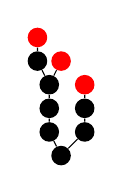
\begin{tikzpicture}[scale=.2]
\node[circle, scale=0.75, fill] (tid0) at (2.25,1.5){};
\node[circle, scale=0.75, fill] (tid1) at (1.5,3){};
\node[circle, scale=0.75, fill] (tid3) at (1.5,4.5){};
\node[circle, scale=0.75, fill] (tid5) at (1.5,6){};
\node[circle, scale=0.75, fill] (tid7) at (0.75,7.5){};
\node[circle, scale=0.75, fill, red] (tid9) at (0.75,9){};
\draw[](tid7) -- (tid9);
\node[circle, scale=0.75, fill, red] (tid8) at (2.25,7.5){};
\draw[](tid5) -- (tid7);
\draw[](tid5) -- (tid8);
\draw[](tid3) -- (tid5);
\draw[](tid1) -- (tid3);
\node[circle, scale=0.75, fill] (tid2) at (3.75,3){};
\node[circle, scale=0.75, fill] (tid4) at (3.75,4.5){};
\node[circle, scale=0.75, fill, red] (tid6) at (3.75,6){};
\draw[](tid4) -- (tid6);
\draw[](tid2) -- (tid4);
\draw[](tid0) -- (tid1);
\draw[](tid0) -- (tid2);
\end{tikzpicture}
\nodepart{two}
\footnotesize{6.56279}
\nodepart{three}
\footnotesize{$33\:33\:33$}
};
 & 
\\
};
\end{scope}
\begin{scope}[yshift=\leveltopIII cm]
\matrix (line3) [column sep=1cm] {
\node[draw=black, rectangle split,  rectangle split parts=3] (sn0x145fad0){
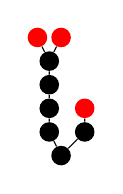
\begin{tikzpicture}[scale=.2]
\node[circle, scale=0.75, fill] (tid0) at (2.25,1.5){};
\node[circle, scale=0.75, fill] (tid1) at (1.5,3){};
\node[circle, scale=0.75, fill] (tid3) at (1.5,4.5){};
\node[circle, scale=0.75, fill] (tid5) at (1.5,6){};
\node[circle, scale=0.75, fill] (tid6) at (1.5,7.5){};
\node[circle, scale=0.75, fill, red] (tid7) at (0.75,9){};
\node[circle, scale=0.75, fill, red] (tid8) at (2.25,9){};
\draw[](tid6) -- (tid7);
\draw[](tid6) -- (tid8);
\draw[](tid5) -- (tid6);
\draw[](tid3) -- (tid5);
\draw[](tid1) -- (tid3);
\node[circle, scale=0.75, fill] (tid2) at (3.75,3){};
\node[circle, scale=0.75, fill, red] (tid4) at (3.75,4.5){};
\draw[](tid2) -- (tid4);
\draw[](tid0) -- (tid1);
\draw[](tid0) -- (tid2);
\end{tikzpicture}
\nodepart{two}
\footnotesize{6.60069}
\nodepart{three}
\footnotesize{$33\:67$}
};
 & 
\node[draw=black, rectangle split,  rectangle split parts=3] (sn0x1460050){
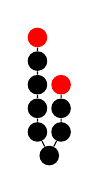
\begin{tikzpicture}[scale=.2]
\node[circle, scale=0.75, fill] (tid0) at (1.5,1.5){};
\node[circle, scale=0.75, fill] (tid1) at (0.75,3){};
\node[circle, scale=0.75, fill] (tid3) at (0.75,4.5){};
\node[circle, scale=0.75, fill] (tid5) at (0.75,6){};
\node[circle, scale=0.75, fill] (tid7) at (0.75,7.5){};
\node[circle, scale=0.75, fill, red] (tid8) at (0.75,9){};
\draw[](tid7) -- (tid8);
\draw[](tid5) -- (tid7);
\draw[](tid3) -- (tid5);
\draw[](tid1) -- (tid3);
\node[circle, scale=0.75, fill] (tid2) at (2.25,3){};
\node[circle, scale=0.75, fill] (tid4) at (2.25,4.5){};
\node[circle, scale=0.75, fill, red] (tid6) at (2.25,6){};
\draw[](tid4) -- (tid6);
\draw[](tid2) -- (tid4);
\draw[](tid0) -- (tid1);
\draw[](tid0) -- (tid2);
\end{tikzpicture}
\nodepart{two}
\footnotesize{6.36719}
\nodepart{three}
\footnotesize{$50\:50$}
};
 & 
\node[draw=black, rectangle split,  rectangle split parts=3] (sn0x1462fe0){
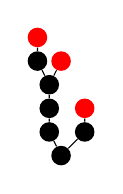
\begin{tikzpicture}[scale=.2]
\node[circle, scale=0.75, fill] (tid0) at (2.25,1.5){};
\node[circle, scale=0.75, fill] (tid1) at (1.5,3){};
\node[circle, scale=0.75, fill] (tid3) at (1.5,4.5){};
\node[circle, scale=0.75, fill] (tid5) at (1.5,6){};
\node[circle, scale=0.75, fill] (tid6) at (0.75,7.5){};
\node[circle, scale=0.75, fill, red] (tid8) at (0.75,9){};
\draw[](tid6) -- (tid8);
\node[circle, scale=0.75, fill, red] (tid7) at (2.25,7.5){};
\draw[](tid5) -- (tid6);
\draw[](tid5) -- (tid7);
\draw[](tid3) -- (tid5);
\draw[](tid1) -- (tid3);
\node[circle, scale=0.75, fill] (tid2) at (3.75,3){};
\node[circle, scale=0.75, fill, red] (tid4) at (3.75,4.5){};
\draw[](tid2) -- (tid4);
\draw[](tid0) -- (tid1);
\draw[](tid0) -- (tid2);
\end{tikzpicture}
\nodepart{two}
\footnotesize{6.36516}
\nodepart{three}
\footnotesize{$33\:33\:33$}
};
 & 
\node[draw=black, rectangle split,  rectangle split parts=3] (sn0x1462bf0){
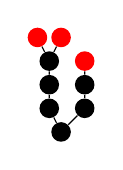
\begin{tikzpicture}[scale=.2]
\node[circle, scale=0.75, fill] (tid0) at (2.25,1.5){};
\node[circle, scale=0.75, fill] (tid1) at (1.5,3){};
\node[circle, scale=0.75, fill] (tid3) at (1.5,4.5){};
\node[circle, scale=0.75, fill] (tid5) at (1.5,6){};
\node[circle, scale=0.75, fill, red] (tid7) at (0.75,7.5){};
\node[circle, scale=0.75, fill, red] (tid8) at (2.25,7.5){};
\draw[](tid5) -- (tid7);
\draw[](tid5) -- (tid8);
\draw[](tid3) -- (tid5);
\draw[](tid1) -- (tid3);
\node[circle, scale=0.75, fill] (tid2) at (3.75,3){};
\node[circle, scale=0.75, fill] (tid4) at (3.75,4.5){};
\node[circle, scale=0.75, fill, red] (tid6) at (3.75,6){};
\draw[](tid4) -- (tid6);
\draw[](tid2) -- (tid4);
\draw[](tid0) -- (tid1);
\draw[](tid0) -- (tid2);
\end{tikzpicture}
\nodepart{two}
\footnotesize{5.95602}
\nodepart{three}
\footnotesize{$67\:33$}
};
 & 
\\
};
\end{scope}
\begin{scope}[yshift=\leveltopIIII cm]
\matrix (line4) [column sep=1cm] {
\node[draw=black, rectangle split,  rectangle split parts=3] (sn0x145e900){
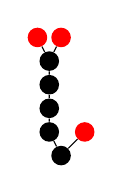
\begin{tikzpicture}[scale=.2]
\node[circle, scale=0.75, fill] (tid0) at (2.25,1.5){};
\node[circle, scale=0.75, fill] (tid1) at (1.5,3){};
\node[circle, scale=0.75, fill] (tid3) at (1.5,4.5){};
\node[circle, scale=0.75, fill] (tid4) at (1.5,6){};
\node[circle, scale=0.75, fill] (tid5) at (1.5,7.5){};
\node[circle, scale=0.75, fill, red] (tid6) at (0.75,9){};
\node[circle, scale=0.75, fill, red] (tid7) at (2.25,9){};
\draw[](tid5) -- (tid6);
\draw[](tid5) -- (tid7);
\draw[](tid4) -- (tid5);
\draw[](tid3) -- (tid4);
\draw[](tid1) -- (tid3);
\node[circle, scale=0.75, fill, red] (tid2) at (3.75,3){};
\draw[](tid0) -- (tid1);
\draw[](tid0) -- (tid2);
\end{tikzpicture}
\nodepart{two}
\footnotesize{6.52083}
\nodepart{three}
\footnotesize{$33\:67$}
};
 & 
\node[draw=black, rectangle split,  rectangle split parts=3] (sn0x145fa00){
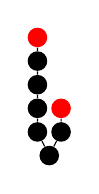
\begin{tikzpicture}[scale=.2]
\node[circle, scale=0.75, fill] (tid0) at (1.5,1.5){};
\node[circle, scale=0.75, fill] (tid1) at (0.75,3){};
\node[circle, scale=0.75, fill] (tid3) at (0.75,4.5){};
\node[circle, scale=0.75, fill] (tid5) at (0.75,6){};
\node[circle, scale=0.75, fill] (tid6) at (0.75,7.5){};
\node[circle, scale=0.75, fill, red] (tid7) at (0.75,9){};
\draw[](tid6) -- (tid7);
\draw[](tid5) -- (tid6);
\draw[](tid3) -- (tid5);
\draw[](tid1) -- (tid3);
\node[circle, scale=0.75, fill] (tid2) at (2.25,3){};
\node[circle, scale=0.75, fill, red] (tid4) at (2.25,4.5){};
\draw[](tid2) -- (tid4);
\draw[](tid0) -- (tid1);
\draw[](tid0) -- (tid2);
\end{tikzpicture}
\nodepart{two}
\footnotesize{6.14062}
\nodepart{three}
\footnotesize{$50\:50$}
};
 & 
\node[draw=black, rectangle split,  rectangle split parts=3] (sn0x145ff80){
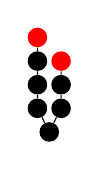
\begin{tikzpicture}[scale=.2]
\node[circle, scale=0.75, fill] (tid0) at (1.5,1.5){};
\node[circle, scale=0.75, fill] (tid1) at (0.75,3){};
\node[circle, scale=0.75, fill] (tid3) at (0.75,4.5){};
\node[circle, scale=0.75, fill] (tid5) at (0.75,6){};
\node[circle, scale=0.75, fill, red] (tid7) at (0.75,7.5){};
\draw[](tid5) -- (tid7);
\draw[](tid3) -- (tid5);
\draw[](tid1) -- (tid3);
\node[circle, scale=0.75, fill] (tid2) at (2.25,3){};
\node[circle, scale=0.75, fill] (tid4) at (2.25,4.5){};
\node[circle, scale=0.75, fill, red] (tid6) at (2.25,6){};
\draw[](tid4) -- (tid6);
\draw[](tid2) -- (tid4);
\draw[](tid0) -- (tid1);
\draw[](tid0) -- (tid2);
\end{tikzpicture}
\nodepart{two}
\footnotesize{5.59375}
\nodepart{three}
\footnotesize{$50\:50$}
};
 & 
\node[draw=black, rectangle split,  rectangle split parts=3] (sn0x1462420){
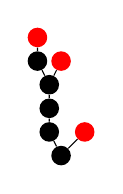
\begin{tikzpicture}[scale=.2]
\node[circle, scale=0.75, fill] (tid0) at (2.25,1.5){};
\node[circle, scale=0.75, fill] (tid1) at (1.5,3){};
\node[circle, scale=0.75, fill] (tid3) at (1.5,4.5){};
\node[circle, scale=0.75, fill] (tid4) at (1.5,6){};
\node[circle, scale=0.75, fill] (tid5) at (0.75,7.5){};
\node[circle, scale=0.75, fill, red] (tid7) at (0.75,9){};
\draw[](tid5) -- (tid7);
\node[circle, scale=0.75, fill, red] (tid6) at (2.25,7.5){};
\draw[](tid4) -- (tid5);
\draw[](tid4) -- (tid6);
\draw[](tid3) -- (tid4);
\draw[](tid1) -- (tid3);
\node[circle, scale=0.75, fill, red] (tid2) at (3.75,3){};
\draw[](tid0) -- (tid1);
\draw[](tid0) -- (tid2);
\end{tikzpicture}
\nodepart{two}
\footnotesize{6.27431}
\nodepart{three}
\footnotesize{$33\:33\:33$}
};
 & 
\node[draw=black, rectangle split,  rectangle split parts=3] (sn0x14624f0){
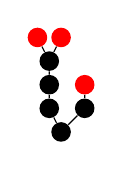
\begin{tikzpicture}[scale=.2]
\node[circle, scale=0.75, fill] (tid0) at (2.25,1.5){};
\node[circle, scale=0.75, fill] (tid1) at (1.5,3){};
\node[circle, scale=0.75, fill] (tid3) at (1.5,4.5){};
\node[circle, scale=0.75, fill] (tid5) at (1.5,6){};
\node[circle, scale=0.75, fill, red] (tid6) at (0.75,7.5){};
\node[circle, scale=0.75, fill, red] (tid7) at (2.25,7.5){};
\draw[](tid5) -- (tid6);
\draw[](tid5) -- (tid7);
\draw[](tid3) -- (tid5);
\draw[](tid1) -- (tid3);
\node[circle, scale=0.75, fill] (tid2) at (3.75,3){};
\node[circle, scale=0.75, fill, red] (tid4) at (3.75,4.5){};
\draw[](tid2) -- (tid4);
\draw[](tid0) -- (tid1);
\draw[](tid0) -- (tid2);
\end{tikzpicture}
\nodepart{two}
\footnotesize{5.68056}
\nodepart{three}
\footnotesize{$67\:33$}
};
 & 
\\
};
\end{scope}
\begin{scope}[yshift=\leveltopIIIII cm]
\matrix (line5) [column sep=1cm] {
\node[draw=black, rectangle split,  rectangle split parts=3] (sn0x145d480){
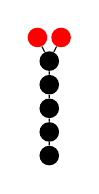
\begin{tikzpicture}[scale=.2]
\node[circle, scale=0.75, fill] (tid0) at (1.5,1.5){};
\node[circle, scale=0.75, fill] (tid1) at (1.5,3){};
\node[circle, scale=0.75, fill] (tid2) at (1.5,4.5){};
\node[circle, scale=0.75, fill] (tid3) at (1.5,6){};
\node[circle, scale=0.75, fill] (tid4) at (1.5,7.5){};
\node[circle, scale=0.75, fill, red] (tid5) at (0.75,9){};
\node[circle, scale=0.75, fill, red] (tid6) at (2.25,9){};
\draw[](tid4) -- (tid5);
\draw[](tid4) -- (tid6);
\draw[](tid3) -- (tid4);
\draw[](tid2) -- (tid3);
\draw[](tid1) -- (tid2);
\draw[](tid0) -- (tid1);
\end{tikzpicture}
\nodepart{two}
\footnotesize{6.5}
\nodepart{three}
\footnotesize{$1$}
};
 & 
\node[draw=black, rectangle split,  rectangle split parts=3] (sn0x145e670){
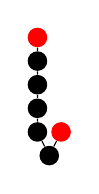
\begin{tikzpicture}[scale=.2]
\node[circle, scale=0.75, fill] (tid0) at (1.5,1.5){};
\node[circle, scale=0.75, fill] (tid1) at (0.75,3){};
\node[circle, scale=0.75, fill] (tid3) at (0.75,4.5){};
\node[circle, scale=0.75, fill] (tid4) at (0.75,6){};
\node[circle, scale=0.75, fill] (tid5) at (0.75,7.5){};
\node[circle, scale=0.75, fill, red] (tid6) at (0.75,9){};
\draw[](tid5) -- (tid6);
\draw[](tid4) -- (tid5);
\draw[](tid3) -- (tid4);
\draw[](tid1) -- (tid3);
\node[circle, scale=0.75, fill, red] (tid2) at (2.25,3){};
\draw[](tid0) -- (tid1);
\draw[](tid0) -- (tid2);
\end{tikzpicture}
\nodepart{two}
\footnotesize{6.03125}
\nodepart{three}
\footnotesize{$50\:50$}
};
 & 
\node[draw=black, rectangle split,  rectangle split parts=3] (sn0x145f770){
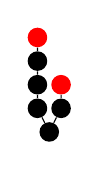
\begin{tikzpicture}[scale=.2]
\node[circle, scale=0.75, fill] (tid0) at (1.5,1.5){};
\node[circle, scale=0.75, fill] (tid1) at (0.75,3){};
\node[circle, scale=0.75, fill] (tid3) at (0.75,4.5){};
\node[circle, scale=0.75, fill] (tid5) at (0.75,6){};
\node[circle, scale=0.75, fill, red] (tid6) at (0.75,7.5){};
\draw[](tid5) -- (tid6);
\draw[](tid3) -- (tid5);
\draw[](tid1) -- (tid3);
\node[circle, scale=0.75, fill] (tid2) at (2.25,3){};
\node[circle, scale=0.75, fill, red] (tid4) at (2.25,4.5){};
\draw[](tid2) -- (tid4);
\draw[](tid0) -- (tid1);
\draw[](tid0) -- (tid2);
\end{tikzpicture}
\nodepart{two}
\footnotesize{5.25}
\nodepart{three}
\footnotesize{$50\:50$}
};
 & 
\node[draw=black, rectangle split,  rectangle split parts=3] (sn0x1460b00){
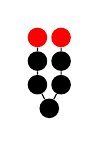
\begin{tikzpicture}[scale=.2]
\node[circle, scale=0.75, fill] (tid0) at (1.5,1.5){};
\node[circle, scale=0.75, fill] (tid1) at (0.75,3){};
\node[circle, scale=0.75, fill] (tid3) at (0.75,4.5){};
\node[circle, scale=0.75, fill, red] (tid5) at (0.75,6){};
\draw[](tid3) -- (tid5);
\draw[](tid1) -- (tid3);
\node[circle, scale=0.75, fill] (tid2) at (2.25,3){};
\node[circle, scale=0.75, fill] (tid4) at (2.25,4.5){};
\node[circle, scale=0.75, fill, red] (tid6) at (2.25,6){};
\draw[](tid4) -- (tid6);
\draw[](tid2) -- (tid4);
\draw[](tid0) -- (tid1);
\draw[](tid0) -- (tid2);
\end{tikzpicture}
\nodepart{two}
\footnotesize{4.9375}
\nodepart{three}
\footnotesize{$1$}
};
 & 
\node[draw=black, rectangle split,  rectangle split parts=3] (sn0x1462350){
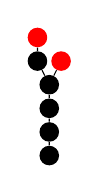
\begin{tikzpicture}[scale=.2]
\node[circle, scale=0.75, fill] (tid0) at (1.5,1.5){};
\node[circle, scale=0.75, fill] (tid1) at (1.5,3){};
\node[circle, scale=0.75, fill] (tid2) at (1.5,4.5){};
\node[circle, scale=0.75, fill] (tid3) at (1.5,6){};
\node[circle, scale=0.75, fill] (tid4) at (0.75,7.5){};
\node[circle, scale=0.75, fill, red] (tid6) at (0.75,9){};
\draw[](tid4) -- (tid6);
\node[circle, scale=0.75, fill, red] (tid5) at (2.25,7.5){};
\draw[](tid3) -- (tid4);
\draw[](tid3) -- (tid5);
\draw[](tid2) -- (tid3);
\draw[](tid1) -- (tid2);
\draw[](tid0) -- (tid1);
\end{tikzpicture}
\nodepart{two}
\footnotesize{6.25}
\nodepart{three}
\footnotesize{$50\:50$}
};
 & 
\node[draw=black, rectangle split,  rectangle split parts=3] (sn0x14628e0){
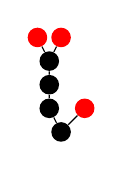
\begin{tikzpicture}[scale=.2]
\node[circle, scale=0.75, fill] (tid0) at (2.25,1.5){};
\node[circle, scale=0.75, fill] (tid1) at (1.5,3){};
\node[circle, scale=0.75, fill] (tid3) at (1.5,4.5){};
\node[circle, scale=0.75, fill] (tid4) at (1.5,6){};
\node[circle, scale=0.75, fill, red] (tid5) at (0.75,7.5){};
\node[circle, scale=0.75, fill, red] (tid6) at (2.25,7.5){};
\draw[](tid4) -- (tid5);
\draw[](tid4) -- (tid6);
\draw[](tid3) -- (tid4);
\draw[](tid1) -- (tid3);
\node[circle, scale=0.75, fill, red] (tid2) at (3.75,3){};
\draw[](tid0) -- (tid1);
\draw[](tid0) -- (tid2);
\end{tikzpicture}
\nodepart{two}
\footnotesize{5.54167}
\nodepart{three}
\footnotesize{$67\:33$}
};
 & 
\\
};
\end{scope}
\begin{scope}[yshift=\leveltopIIIIII cm]
\matrix (line6) [column sep=1cm] {
\node[draw=black, rectangle split,  rectangle split parts=3] (sn0x145d0f0){
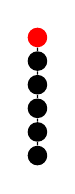
\begin{tikzpicture}[scale=.2]
\node[circle, scale=0.75, fill] (tid0) at (0.75,1.5){};
\node[circle, scale=0.75, fill] (tid1) at (0.75,3){};
\node[circle, scale=0.75, fill] (tid2) at (0.75,4.5){};
\node[circle, scale=0.75, fill] (tid3) at (0.75,6){};
\node[circle, scale=0.75, fill] (tid4) at (0.75,7.5){};
\node[circle, scale=0.75, fill, red] (tid5) at (0.75,9){};
\draw[](tid4) -- (tid5);
\draw[](tid3) -- (tid4);
\draw[](tid2) -- (tid3);
\draw[](tid1) -- (tid2);
\draw[](tid0) -- (tid1);
\end{tikzpicture}
\nodepart{two}
\footnotesize{6}
\nodepart{three}
\footnotesize{$1$}
};
 & 
\node[draw=black, rectangle split,  rectangle split parts=3] (sn0x145e380){
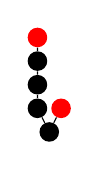
\begin{tikzpicture}[scale=.2]
\node[circle, scale=0.75, fill] (tid0) at (1.5,1.5){};
\node[circle, scale=0.75, fill] (tid1) at (0.75,3){};
\node[circle, scale=0.75, fill] (tid3) at (0.75,4.5){};
\node[circle, scale=0.75, fill] (tid4) at (0.75,6){};
\node[circle, scale=0.75, fill, red] (tid5) at (0.75,7.5){};
\draw[](tid4) -- (tid5);
\draw[](tid3) -- (tid4);
\draw[](tid1) -- (tid3);
\node[circle, scale=0.75, fill, red] (tid2) at (2.25,3){};
\draw[](tid0) -- (tid1);
\draw[](tid0) -- (tid2);
\end{tikzpicture}
\nodepart{two}
\footnotesize{5.0625}
\nodepart{three}
\footnotesize{$50\:50$}
};
 & 
\node[draw=black, rectangle split,  rectangle split parts=3] (sn0x145ec40){
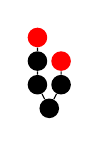
\begin{tikzpicture}[scale=.2]
\node[circle, scale=0.75, fill] (tid0) at (1.5,1.5){};
\node[circle, scale=0.75, fill] (tid1) at (0.75,3){};
\node[circle, scale=0.75, fill] (tid3) at (0.75,4.5){};
\node[circle, scale=0.75, fill, red] (tid5) at (0.75,6){};
\draw[](tid3) -- (tid5);
\draw[](tid1) -- (tid3);
\node[circle, scale=0.75, fill] (tid2) at (2.25,3){};
\node[circle, scale=0.75, fill, red] (tid4) at (2.25,4.5){};
\draw[](tid2) -- (tid4);
\draw[](tid0) -- (tid1);
\draw[](tid0) -- (tid2);
\end{tikzpicture}
\nodepart{two}
\footnotesize{4.4375}
\nodepart{three}
\footnotesize{$50\:50$}
};
 & 
\node[draw=black, rectangle split,  rectangle split parts=3] (sn0x1461150){
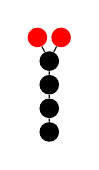
\begin{tikzpicture}[scale=.2]
\node[circle, scale=0.75, fill] (tid0) at (1.5,1.5){};
\node[circle, scale=0.75, fill] (tid1) at (1.5,3){};
\node[circle, scale=0.75, fill] (tid2) at (1.5,4.5){};
\node[circle, scale=0.75, fill] (tid3) at (1.5,6){};
\node[circle, scale=0.75, fill, red] (tid4) at (0.75,7.5){};
\node[circle, scale=0.75, fill, red] (tid5) at (2.25,7.5){};
\draw[](tid3) -- (tid4);
\draw[](tid3) -- (tid5);
\draw[](tid2) -- (tid3);
\draw[](tid1) -- (tid2);
\draw[](tid0) -- (tid1);
\end{tikzpicture}
\nodepart{two}
\footnotesize{5.5}
\nodepart{three}
\footnotesize{$1$}
};
 & 
\\
};
\end{scope}
\begin{scope}[yshift=\leveltopIIIIIII cm]
\matrix (line7) [column sep=1cm] {
\node[draw=black, rectangle split,  rectangle split parts=3] (sn0x145cdf0){
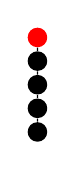
\begin{tikzpicture}[scale=.2]
\node[circle, scale=0.75, fill] (tid0) at (0.75,1.5){};
\node[circle, scale=0.75, fill] (tid1) at (0.75,3){};
\node[circle, scale=0.75, fill] (tid2) at (0.75,4.5){};
\node[circle, scale=0.75, fill] (tid3) at (0.75,6){};
\node[circle, scale=0.75, fill, red] (tid4) at (0.75,7.5){};
\draw[](tid3) -- (tid4);
\draw[](tid2) -- (tid3);
\draw[](tid1) -- (tid2);
\draw[](tid0) -- (tid1);
\end{tikzpicture}
\nodepart{two}
\footnotesize{5}
\nodepart{three}
\footnotesize{$1$}
};
 & 
\node[draw=black, rectangle split,  rectangle split parts=3] (sn0x145e0d0){
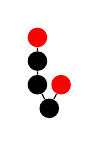
\begin{tikzpicture}[scale=.2]
\node[circle, scale=0.75, fill] (tid0) at (1.5,1.5){};
\node[circle, scale=0.75, fill] (tid1) at (0.75,3){};
\node[circle, scale=0.75, fill] (tid3) at (0.75,4.5){};
\node[circle, scale=0.75, fill, red] (tid4) at (0.75,6){};
\draw[](tid3) -- (tid4);
\draw[](tid1) -- (tid3);
\node[circle, scale=0.75, fill, red] (tid2) at (2.25,3){};
\draw[](tid0) -- (tid1);
\draw[](tid0) -- (tid2);
\end{tikzpicture}
\nodepart{two}
\footnotesize{4.125}
\nodepart{three}
\footnotesize{$50\:50$}
};
 & 
\node[draw=black, rectangle split,  rectangle split parts=3] (sn0x145eb50){
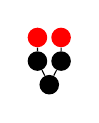
\begin{tikzpicture}[scale=.2]
\node[circle, scale=0.75, fill] (tid0) at (1.5,1.5){};
\node[circle, scale=0.75, fill] (tid1) at (0.75,3){};
\node[circle, scale=0.75, fill, red] (tid3) at (0.75,4.5){};
\draw[](tid1) -- (tid3);
\node[circle, scale=0.75, fill] (tid2) at (2.25,3){};
\node[circle, scale=0.75, fill, red] (tid4) at (2.25,4.5){};
\draw[](tid2) -- (tid4);
\draw[](tid0) -- (tid1);
\draw[](tid0) -- (tid2);
\end{tikzpicture}
\nodepart{two}
\footnotesize{3.75}
\nodepart{three}
\footnotesize{$1$}
};
 & 
\\
};
\end{scope}
\begin{scope}[yshift=\leveltopIIIIIIII cm]
\matrix (line8) [column sep=1cm] {
\node[draw=black, rectangle split,  rectangle split parts=3] (sn0x145cd20){
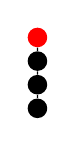
\begin{tikzpicture}[scale=.2]
\node[circle, scale=0.75, fill] (tid0) at (0.75,1.5){};
\node[circle, scale=0.75, fill] (tid1) at (0.75,3){};
\node[circle, scale=0.75, fill] (tid2) at (0.75,4.5){};
\node[circle, scale=0.75, fill, red] (tid3) at (0.75,6){};
\draw[](tid2) -- (tid3);
\draw[](tid1) -- (tid2);
\draw[](tid0) -- (tid1);
\end{tikzpicture}
\nodepart{two}
\footnotesize{4}
\nodepart{three}
\footnotesize{$1$}
};
 & 
\node[draw=black, rectangle split,  rectangle split parts=3] (sn0x145d820){
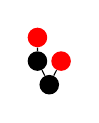
\begin{tikzpicture}[scale=.2]
\node[circle, scale=0.75, fill] (tid0) at (1.5,1.5){};
\node[circle, scale=0.75, fill] (tid1) at (0.75,3){};
\node[circle, scale=0.75, fill, red] (tid3) at (0.75,4.5){};
\draw[](tid1) -- (tid3);
\node[circle, scale=0.75, fill, red] (tid2) at (2.25,3){};
\draw[](tid0) -- (tid1);
\draw[](tid0) -- (tid2);
\end{tikzpicture}
\nodepart{two}
\footnotesize{3.25}
\nodepart{three}
\footnotesize{$50\:50$}
};
 & 
\\
};
\end{scope}
\begin{scope}[yshift=\leveltopIIIIIIIII cm]
\matrix (line9) [column sep=1cm] {
\node[draw=black, rectangle split,  rectangle split parts=3] (sn0x145b6b0){
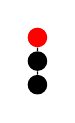
\begin{tikzpicture}[scale=.2]
\node[circle, scale=0.75, fill] (tid0) at (0.75,1.5){};
\node[circle, scale=0.75, fill] (tid1) at (0.75,3){};
\node[circle, scale=0.75, fill, red] (tid2) at (0.75,4.5){};
\draw[](tid1) -- (tid2);
\draw[](tid0) -- (tid1);
\end{tikzpicture}
\nodepart{two}
\footnotesize{3}
\nodepart{three}
\footnotesize{$1$}
};
 & 
\node[draw=black, rectangle split,  rectangle split parts=3] (sn0x145d710){

\begin{tikzpicture}[scale=.2]
\node[circle, scale=0.75, fill] (tid0) at (1.5,1.5){};
\node[circle, scale=0.75, fill, red] (tid1) at (0.75,3){};
\node[circle, scale=0.75, fill, red] (tid2) at (2.25,3){};
\draw[](tid0) -- (tid1);
\draw[](tid0) -- (tid2);
\end{tikzpicture}
\nodepart{two}
\footnotesize{2.5}
\nodepart{three}
\footnotesize{$1$}
};
 & 
\\
};
\end{scope}
\begin{scope}[yshift=\leveltopIIIIIIIIII cm]
\matrix (line10) [column sep=1cm] {
\node[draw=black, rectangle split,  rectangle split parts=3] (sn0x145aea0){
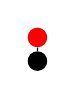
\begin{tikzpicture}[scale=.2]
\node[circle, scale=0.75, fill] (tid0) at (0.75,1.5){};
\node[circle, scale=0.75, fill, red] (tid1) at (0.75,3){};
\draw[](tid0) -- (tid1);
\end{tikzpicture}
\nodepart{two}
\footnotesize{2}
\nodepart{three}
\footnotesize{$1$}
};
 & 
\\
};
\end{scope}
\begin{scope}[yshift=\leveltopIIIIIIIIIII cm]
\matrix (line11) [column sep=1cm] {
\node[draw=black, rectangle split,  rectangle split parts=3] (sn0x145b5e0){

\begin{tikzpicture}[scale=.2]
\node[circle, scale=0.75, fill, red] (tid0) at (0.75,1.5){};
\end{tikzpicture}
\nodepart{two}
\footnotesize{1}
\nodepart{three}
\footnotesize{$$}
};
 & 
\\
};
\end{scope}
\begin{scope}[yshift=\leveltopIIIIIIIIIIII cm]
\matrix (line12) [column sep=1cm] {
\\
};
\end{scope}
\draw (sn0x14639f0.south) -- (sn0x1460d30.north);
\draw (sn0x14639f0.south) -- (sn0x14633d0.north);
\draw (sn0x1460d30.south) -- (sn0x145fad0.north);
\draw (sn0x1460d30.south) -- (sn0x1460050.north);
\draw (sn0x14633d0.south) -- (sn0x1462fe0.north);
\draw (sn0x14633d0.south) -- (sn0x1460050.north);
\draw (sn0x14633d0.south) -- (sn0x1462bf0.north);
\draw (sn0x145fad0.south) -- (sn0x145e900.north);
\draw (sn0x145fad0.south) -- (sn0x145fa00.north);
\draw (sn0x1460050.south) -- (sn0x145fa00.north);
\draw (sn0x1460050.south) -- (sn0x145ff80.north);
\draw (sn0x1462fe0.south) -- (sn0x1462420.north);
\draw (sn0x1462fe0.south) -- (sn0x145fa00.north);
\draw (sn0x1462fe0.south) -- (sn0x14624f0.north);
\draw (sn0x1462bf0.south) -- (sn0x14624f0.north);
\draw (sn0x1462bf0.south) -- (sn0x145ff80.north);
\draw (sn0x145e900.south) -- (sn0x145d480.north);
\draw (sn0x145e900.south) -- (sn0x145e670.north);
\draw (sn0x145fa00.south) -- (sn0x145e670.north);
\draw (sn0x145fa00.south) -- (sn0x145f770.north);
\draw (sn0x145ff80.south) -- (sn0x145f770.north);
\draw (sn0x145ff80.south) -- (sn0x1460b00.north);
\draw (sn0x1462420.south) -- (sn0x1462350.north);
\draw (sn0x1462420.south) -- (sn0x145e670.north);
\draw (sn0x1462420.south) -- (sn0x14628e0.north);
\draw (sn0x14624f0.south) -- (sn0x14628e0.north);
\draw (sn0x14624f0.south) -- (sn0x145f770.north);
\draw (sn0x145d480.south) -- (sn0x145d0f0.north);
\draw (sn0x145e670.south) -- (sn0x145d0f0.north);
\draw (sn0x145e670.south) -- (sn0x145e380.north);
\draw (sn0x145f770.south) -- (sn0x145e380.north);
\draw (sn0x145f770.south) -- (sn0x145ec40.north);
\draw (sn0x1460b00.south) -- (sn0x145ec40.north);
\draw (sn0x1462350.south) -- (sn0x145d0f0.north);
\draw (sn0x1462350.south) -- (sn0x1461150.north);
\draw (sn0x14628e0.south) -- (sn0x1461150.north);
\draw (sn0x14628e0.south) -- (sn0x145e380.north);
\draw (sn0x145d0f0.south) -- (sn0x145cdf0.north);
\draw (sn0x145e380.south) -- (sn0x145cdf0.north);
\draw (sn0x145e380.south) -- (sn0x145e0d0.north);
\draw (sn0x145ec40.south) -- (sn0x145e0d0.north);
\draw (sn0x145ec40.south) -- (sn0x145eb50.north);
\draw (sn0x1461150.south) -- (sn0x145cdf0.north);
\draw (sn0x145cdf0.south) -- (sn0x145cd20.north);
\draw (sn0x145e0d0.south) -- (sn0x145cd20.north);
\draw (sn0x145e0d0.south) -- (sn0x145d820.north);
\draw (sn0x145eb50.south) -- (sn0x145d820.north);
\draw (sn0x145cd20.south) -- (sn0x145b6b0.north);
\draw (sn0x145d820.south) -- (sn0x145b6b0.north);
\draw (sn0x145d820.south) -- (sn0x145d710.north);
\draw (sn0x145b6b0.south) -- (sn0x145aea0.north);
\draw (sn0x145d710.south) -- (sn0x145aea0.north);
\draw (sn0x145aea0.south) -- (sn0x145b5e0.north);
\end{tikzpicture}

%%% Local Variables:
%%% TeX-master: "thesis/thesis.tex"
%%% End: 

  \renewcommand{\leveltopI}{-15cm + \leveltop}
\renewcommand{\leveltopII}{-15cm + \leveltopI}
\renewcommand{\leveltopIII}{-15cm + \leveltopII}
\renewcommand{\leveltopIIII}{-15cm + \leveltopIII}
\renewcommand{\leveltopIIIII}{-15cm + \leveltopIIII}
\renewcommand{\leveltopIIIIII}{-15cm + \leveltopIIIII}
\renewcommand{\leveltopIIIIIII}{-15cm + \leveltopIIIIII}
\renewcommand{\leveltopIIIIIIII}{-15cm + \leveltopIIIIIII}
\renewcommand{\leveltopIIIIIIIII}{-15cm + \leveltopIIIIIIII}
\renewcommand{\leveltopIIIIIIIIII}{-15cm + \leveltopIIIIIIIII}
\renewcommand{\leveltopIIIIIIIIIII}{-15cm + \leveltopIIIIIIIIII}
\begin{tikzpicture}[scale=.2, anchor=south]
\begin{scope}[yshift=\leveltopI cm]
\matrix (line1) [column sep=1cm] {
\node[draw=black, rectangle split,  rectangle split parts=4] (sn0x18908d0){
\footnotesize{1}
\nodepart{two}
\begin{tikzpicture}[scale=.2]
\node[circle, scale=0.75, fill] (tid0) at (3,1.5){};
\node[circle, scale=0.75, fill] (tid1) at (2.25,3){};
\node[circle, scale=0.75, fill] (tid3) at (2.25,4.5){};
\node[circle, scale=0.75, fill] (tid5) at (2.25,6){};
\node[circle, scale=0.75, fill] (tid7) at (1.5,7.5){};
\node[circle, scale=0.75, fill, red] (tid9) at (0.75,9){};
\node[circle, scale=0.75, fill, red] (tid10) at (2.25,9){};
\draw[](tid7) -- (tid9);
\draw[](tid7) -- (tid10);
\node[circle, scale=0.75, fill] (tid8) at (3.75,7.5){};
\draw[](tid5) -- (tid7);
\draw[](tid5) -- (tid8);
\draw[](tid3) -- (tid5);
\draw[](tid1) -- (tid3);
\node[circle, scale=0.75, fill] (tid2) at (5.25,3){};
\node[circle, scale=0.75, fill] (tid4) at (5.25,4.5){};
\node[circle, scale=0.75, fill, red] (tid6) at (5.25,6){};
\draw[](tid4) -- (tid6);
\draw[](tid2) -- (tid4);
\draw[](tid0) -- (tid1);
\draw[](tid0) -- (tid2);
\end{tikzpicture}
\nodepart{three}
\footnotesize{6.96753}
\nodepart{four}
\footnotesize{$33\:67$}
};
 & 
\\
};
\end{scope}
\begin{scope}[yshift=\leveltopII cm]
\matrix (line2) [column sep=1cm] {
\node[draw=black, rectangle split,  rectangle split parts=4] (sn0x188ec30){
\footnotesize{0.333333}
\nodepart{two}
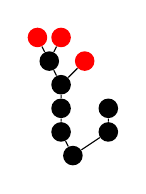
\begin{tikzpicture}[scale=.2]
\node[circle, scale=0.75, fill] (tid0) at (3,1.5){};
\node[circle, scale=0.75, fill] (tid1) at (2.25,3){};
\node[circle, scale=0.75, fill] (tid3) at (2.25,4.5){};
\node[circle, scale=0.75, fill] (tid5) at (2.25,6){};
\node[circle, scale=0.75, fill] (tid6) at (1.5,7.5){};
\node[circle, scale=0.75, fill, red] (tid8) at (0.75,9){};
\node[circle, scale=0.75, fill, red] (tid9) at (2.25,9){};
\draw[](tid6) -- (tid8);
\draw[](tid6) -- (tid9);
\node[circle, scale=0.75, fill, red] (tid7) at (3.75,7.5){};
\draw[](tid5) -- (tid6);
\draw[](tid5) -- (tid7);
\draw[](tid3) -- (tid5);
\draw[](tid1) -- (tid3);
\node[circle, scale=0.75, fill] (tid2) at (5.25,3){};
\node[circle, scale=0.75, fill] (tid4) at (5.25,4.5){};
\draw[](tid2) -- (tid4);
\draw[](tid0) -- (tid1);
\draw[](tid0) -- (tid2);
\end{tikzpicture}
\nodepart{three}
\footnotesize{6.77701}
\nodepart{four}
\footnotesize{$33\:67$}
};
 & 
\node[draw=black, rectangle split,  rectangle split parts=4] (sn0x18906a0){
\footnotesize{0.666667}
\nodepart{two}
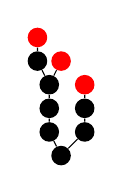
\begin{tikzpicture}[scale=.2]
\node[circle, scale=0.75, fill] (tid0) at (2.25,1.5){};
\node[circle, scale=0.75, fill] (tid1) at (1.5,3){};
\node[circle, scale=0.75, fill] (tid3) at (1.5,4.5){};
\node[circle, scale=0.75, fill] (tid5) at (1.5,6){};
\node[circle, scale=0.75, fill] (tid7) at (0.75,7.5){};
\node[circle, scale=0.75, fill, red] (tid9) at (0.75,9){};
\draw[](tid7) -- (tid9);
\node[circle, scale=0.75, fill, red] (tid8) at (2.25,7.5){};
\draw[](tid5) -- (tid7);
\draw[](tid5) -- (tid8);
\draw[](tid3) -- (tid5);
\draw[](tid1) -- (tid3);
\node[circle, scale=0.75, fill] (tid2) at (3.75,3){};
\node[circle, scale=0.75, fill] (tid4) at (3.75,4.5){};
\node[circle, scale=0.75, fill, red] (tid6) at (3.75,6){};
\draw[](tid4) -- (tid6);
\draw[](tid2) -- (tid4);
\draw[](tid0) -- (tid1);
\draw[](tid0) -- (tid2);
\end{tikzpicture}
\nodepart{three}
\footnotesize{6.56279}
\nodepart{four}
\footnotesize{$33\:33\:33$}
};
 & 
\\
};
\end{scope}
\begin{scope}[yshift=\leveltopIII cm]
\matrix (line3) [column sep=1cm] {
\node[draw=black, rectangle split,  rectangle split parts=4] (sn0x188e220){
\footnotesize{0.111111}
\nodepart{two}
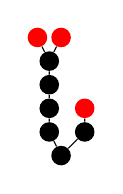
\begin{tikzpicture}[scale=.2]
\node[circle, scale=0.75, fill] (tid0) at (2.25,1.5){};
\node[circle, scale=0.75, fill] (tid1) at (1.5,3){};
\node[circle, scale=0.75, fill] (tid3) at (1.5,4.5){};
\node[circle, scale=0.75, fill] (tid5) at (1.5,6){};
\node[circle, scale=0.75, fill] (tid6) at (1.5,7.5){};
\node[circle, scale=0.75, fill, red] (tid7) at (0.75,9){};
\node[circle, scale=0.75, fill, red] (tid8) at (2.25,9){};
\draw[](tid6) -- (tid7);
\draw[](tid6) -- (tid8);
\draw[](tid5) -- (tid6);
\draw[](tid3) -- (tid5);
\draw[](tid1) -- (tid3);
\node[circle, scale=0.75, fill] (tid2) at (3.75,3){};
\node[circle, scale=0.75, fill, red] (tid4) at (3.75,4.5){};
\draw[](tid2) -- (tid4);
\draw[](tid0) -- (tid1);
\draw[](tid0) -- (tid2);
\end{tikzpicture}
\nodepart{three}
\footnotesize{6.60069}
\nodepart{four}
\footnotesize{$33\:67$}
};
 & 
\node[draw=black, rectangle split,  rectangle split parts=4] (sn0x188d8a0){
\footnotesize{0.444444}
\nodepart{two}
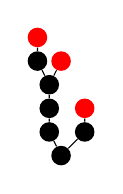
\begin{tikzpicture}[scale=.2]
\node[circle, scale=0.75, fill] (tid0) at (2.25,1.5){};
\node[circle, scale=0.75, fill] (tid1) at (1.5,3){};
\node[circle, scale=0.75, fill] (tid3) at (1.5,4.5){};
\node[circle, scale=0.75, fill] (tid5) at (1.5,6){};
\node[circle, scale=0.75, fill] (tid6) at (0.75,7.5){};
\node[circle, scale=0.75, fill, red] (tid8) at (0.75,9){};
\draw[](tid6) -- (tid8);
\node[circle, scale=0.75, fill, red] (tid7) at (2.25,7.5){};
\draw[](tid5) -- (tid6);
\draw[](tid5) -- (tid7);
\draw[](tid3) -- (tid5);
\draw[](tid1) -- (tid3);
\node[circle, scale=0.75, fill] (tid2) at (3.75,3){};
\node[circle, scale=0.75, fill, red] (tid4) at (3.75,4.5){};
\draw[](tid2) -- (tid4);
\draw[](tid0) -- (tid1);
\draw[](tid0) -- (tid2);
\end{tikzpicture}
\nodepart{three}
\footnotesize{6.36516}
\nodepart{four}
\footnotesize{$33\:33\:33$}
};
 & 
\node[draw=black, rectangle split,  rectangle split parts=4] (sn0x188f0f0){
\footnotesize{0.222222}
\nodepart{two}
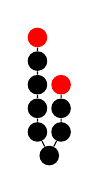
\begin{tikzpicture}[scale=.2]
\node[circle, scale=0.75, fill] (tid0) at (1.5,1.5){};
\node[circle, scale=0.75, fill] (tid1) at (0.75,3){};
\node[circle, scale=0.75, fill] (tid3) at (0.75,4.5){};
\node[circle, scale=0.75, fill] (tid5) at (0.75,6){};
\node[circle, scale=0.75, fill] (tid7) at (0.75,7.5){};
\node[circle, scale=0.75, fill, red] (tid8) at (0.75,9){};
\draw[](tid7) -- (tid8);
\draw[](tid5) -- (tid7);
\draw[](tid3) -- (tid5);
\draw[](tid1) -- (tid3);
\node[circle, scale=0.75, fill] (tid2) at (2.25,3){};
\node[circle, scale=0.75, fill] (tid4) at (2.25,4.5){};
\node[circle, scale=0.75, fill, red] (tid6) at (2.25,6){};
\draw[](tid4) -- (tid6);
\draw[](tid2) -- (tid4);
\draw[](tid0) -- (tid1);
\draw[](tid0) -- (tid2);
\end{tikzpicture}
\nodepart{three}
\footnotesize{6.36719}
\nodepart{four}
\footnotesize{$50\:50$}
};
 & 
\node[draw=black, rectangle split,  rectangle split parts=4] (sn0x188ff90){
\footnotesize{0.222222}
\nodepart{two}
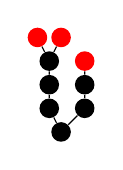
\begin{tikzpicture}[scale=.2]
\node[circle, scale=0.75, fill] (tid0) at (2.25,1.5){};
\node[circle, scale=0.75, fill] (tid1) at (1.5,3){};
\node[circle, scale=0.75, fill] (tid3) at (1.5,4.5){};
\node[circle, scale=0.75, fill] (tid5) at (1.5,6){};
\node[circle, scale=0.75, fill, red] (tid7) at (0.75,7.5){};
\node[circle, scale=0.75, fill, red] (tid8) at (2.25,7.5){};
\draw[](tid5) -- (tid7);
\draw[](tid5) -- (tid8);
\draw[](tid3) -- (tid5);
\draw[](tid1) -- (tid3);
\node[circle, scale=0.75, fill] (tid2) at (3.75,3){};
\node[circle, scale=0.75, fill] (tid4) at (3.75,4.5){};
\node[circle, scale=0.75, fill, red] (tid6) at (3.75,6){};
\draw[](tid4) -- (tid6);
\draw[](tid2) -- (tid4);
\draw[](tid0) -- (tid1);
\draw[](tid0) -- (tid2);
\end{tikzpicture}
\nodepart{three}
\footnotesize{5.95602}
\nodepart{four}
\footnotesize{$33\:67$}
};
 & 
\\
};
\end{scope}
\begin{scope}[yshift=\leveltopIIII cm]
\matrix (line4) [column sep=1cm] {
\node[draw=black, rectangle split,  rectangle split parts=4] (sn0x188c370){
\footnotesize{0.037037}
\nodepart{two}
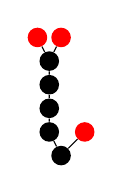
\begin{tikzpicture}[scale=.2]
\node[circle, scale=0.75, fill] (tid0) at (2.25,1.5){};
\node[circle, scale=0.75, fill] (tid1) at (1.5,3){};
\node[circle, scale=0.75, fill] (tid3) at (1.5,4.5){};
\node[circle, scale=0.75, fill] (tid4) at (1.5,6){};
\node[circle, scale=0.75, fill] (tid5) at (1.5,7.5){};
\node[circle, scale=0.75, fill, red] (tid6) at (0.75,9){};
\node[circle, scale=0.75, fill, red] (tid7) at (2.25,9){};
\draw[](tid5) -- (tid6);
\draw[](tid5) -- (tid7);
\draw[](tid4) -- (tid5);
\draw[](tid3) -- (tid4);
\draw[](tid1) -- (tid3);
\node[circle, scale=0.75, fill, red] (tid2) at (3.75,3){};
\draw[](tid0) -- (tid1);
\draw[](tid0) -- (tid2);
\end{tikzpicture}
\nodepart{three}
\footnotesize{6.52083}
\nodepart{four}
\footnotesize{$33\:67$}
};
 & 
\node[draw=black, rectangle split,  rectangle split parts=4] (sn0x188d690){
\footnotesize{0.333333}
\nodepart{two}
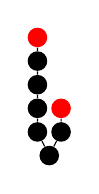
\begin{tikzpicture}[scale=.2]
\node[circle, scale=0.75, fill] (tid0) at (1.5,1.5){};
\node[circle, scale=0.75, fill] (tid1) at (0.75,3){};
\node[circle, scale=0.75, fill] (tid3) at (0.75,4.5){};
\node[circle, scale=0.75, fill] (tid5) at (0.75,6){};
\node[circle, scale=0.75, fill] (tid6) at (0.75,7.5){};
\node[circle, scale=0.75, fill, red] (tid7) at (0.75,9){};
\draw[](tid6) -- (tid7);
\draw[](tid5) -- (tid6);
\draw[](tid3) -- (tid5);
\draw[](tid1) -- (tid3);
\node[circle, scale=0.75, fill] (tid2) at (2.25,3){};
\node[circle, scale=0.75, fill, red] (tid4) at (2.25,4.5){};
\draw[](tid2) -- (tid4);
\draw[](tid0) -- (tid1);
\draw[](tid0) -- (tid2);
\end{tikzpicture}
\nodepart{three}
\footnotesize{6.14062}
\nodepart{four}
\footnotesize{$50\:50$}
};
 & 
\node[draw=black, rectangle split,  rectangle split parts=4] (sn0x188b180){
\footnotesize{0.148148}
\nodepart{two}
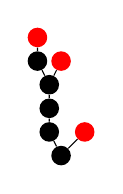
\begin{tikzpicture}[scale=.2]
\node[circle, scale=0.75, fill] (tid0) at (2.25,1.5){};
\node[circle, scale=0.75, fill] (tid1) at (1.5,3){};
\node[circle, scale=0.75, fill] (tid3) at (1.5,4.5){};
\node[circle, scale=0.75, fill] (tid4) at (1.5,6){};
\node[circle, scale=0.75, fill] (tid5) at (0.75,7.5){};
\node[circle, scale=0.75, fill, red] (tid7) at (0.75,9){};
\draw[](tid5) -- (tid7);
\node[circle, scale=0.75, fill, red] (tid6) at (2.25,7.5){};
\draw[](tid4) -- (tid5);
\draw[](tid4) -- (tid6);
\draw[](tid3) -- (tid4);
\draw[](tid1) -- (tid3);
\node[circle, scale=0.75, fill, red] (tid2) at (3.75,3){};
\draw[](tid0) -- (tid1);
\draw[](tid0) -- (tid2);
\end{tikzpicture}
\nodepart{three}
\footnotesize{6.27431}
\nodepart{four}
\footnotesize{$33\:33\:33$}
};
 & 
\node[draw=black, rectangle split,  rectangle split parts=4] (sn0x188de90){
\footnotesize{0.222222}
\nodepart{two}
\begin{tikzpicture}[scale=.2]
\node[circle, scale=0.75, fill] (tid0) at (2.25,1.5){};
\node[circle, scale=0.75, fill] (tid1) at (1.5,3){};
\node[circle, scale=0.75, fill] (tid3) at (1.5,4.5){};
\node[circle, scale=0.75, fill] (tid5) at (1.5,6){};
\node[circle, scale=0.75, fill, red] (tid6) at (0.75,7.5){};
\node[circle, scale=0.75, fill, red] (tid7) at (2.25,7.5){};
\draw[](tid5) -- (tid6);
\draw[](tid5) -- (tid7);
\draw[](tid3) -- (tid5);
\draw[](tid1) -- (tid3);
\node[circle, scale=0.75, fill] (tid2) at (3.75,3){};
\node[circle, scale=0.75, fill, red] (tid4) at (3.75,4.5){};
\draw[](tid2) -- (tid4);
\draw[](tid0) -- (tid1);
\draw[](tid0) -- (tid2);
\end{tikzpicture}
\nodepart{three}
\footnotesize{5.68056}
\nodepart{four}
\footnotesize{$67\:33$}
};
 & 
\node[draw=black, rectangle split,  rectangle split parts=4] (sn0x188f020){
\footnotesize{0.259259}
\nodepart{two}
\begin{tikzpicture}[scale=.2]
\node[circle, scale=0.75, fill] (tid0) at (1.5,1.5){};
\node[circle, scale=0.75, fill] (tid1) at (0.75,3){};
\node[circle, scale=0.75, fill] (tid3) at (0.75,4.5){};
\node[circle, scale=0.75, fill] (tid5) at (0.75,6){};
\node[circle, scale=0.75, fill, red] (tid7) at (0.75,7.5){};
\draw[](tid5) -- (tid7);
\draw[](tid3) -- (tid5);
\draw[](tid1) -- (tid3);
\node[circle, scale=0.75, fill] (tid2) at (2.25,3){};
\node[circle, scale=0.75, fill] (tid4) at (2.25,4.5){};
\node[circle, scale=0.75, fill, red] (tid6) at (2.25,6){};
\draw[](tid4) -- (tid6);
\draw[](tid2) -- (tid4);
\draw[](tid0) -- (tid1);
\draw[](tid0) -- (tid2);
\end{tikzpicture}
\nodepart{three}
\footnotesize{5.59375}
\nodepart{four}
\footnotesize{$50\:50$}
};
 & 
\\
};
\end{scope}
\begin{scope}[yshift=\leveltopIIIII cm]
\matrix (line5) [column sep=1cm] {
\node[draw=black, rectangle split,  rectangle split parts=4] (sn0x1888fa0){
\footnotesize{0.0123457}
\nodepart{two}
\begin{tikzpicture}[scale=.2]
\node[circle, scale=0.75, fill] (tid0) at (1.5,1.5){};
\node[circle, scale=0.75, fill] (tid1) at (1.5,3){};
\node[circle, scale=0.75, fill] (tid2) at (1.5,4.5){};
\node[circle, scale=0.75, fill] (tid3) at (1.5,6){};
\node[circle, scale=0.75, fill] (tid4) at (1.5,7.5){};
\node[circle, scale=0.75, fill, red] (tid5) at (0.75,9){};
\node[circle, scale=0.75, fill, red] (tid6) at (2.25,9){};
\draw[](tid4) -- (tid5);
\draw[](tid4) -- (tid6);
\draw[](tid3) -- (tid4);
\draw[](tid2) -- (tid3);
\draw[](tid1) -- (tid2);
\draw[](tid0) -- (tid1);
\end{tikzpicture}
\nodepart{three}
\footnotesize{6.5}
\nodepart{four}
\footnotesize{$1$}
};
 & 
\node[draw=black, rectangle split,  rectangle split parts=4] (sn0x188ae00){
\footnotesize{0.240741}
\nodepart{two}
\begin{tikzpicture}[scale=.2]
\node[circle, scale=0.75, fill] (tid0) at (1.5,1.5){};
\node[circle, scale=0.75, fill] (tid1) at (0.75,3){};
\node[circle, scale=0.75, fill] (tid3) at (0.75,4.5){};
\node[circle, scale=0.75, fill] (tid4) at (0.75,6){};
\node[circle, scale=0.75, fill] (tid5) at (0.75,7.5){};
\node[circle, scale=0.75, fill, red] (tid6) at (0.75,9){};
\draw[](tid5) -- (tid6);
\draw[](tid4) -- (tid5);
\draw[](tid3) -- (tid4);
\draw[](tid1) -- (tid3);
\node[circle, scale=0.75, fill, red] (tid2) at (2.25,3){};
\draw[](tid0) -- (tid1);
\draw[](tid0) -- (tid2);
\end{tikzpicture}
\nodepart{three}
\footnotesize{6.03125}
\nodepart{four}
\footnotesize{$50\:50$}
};
 & 
\node[draw=black, rectangle split,  rectangle split parts=4] (sn0x188d460){
\footnotesize{0.444444}
\nodepart{two}
\begin{tikzpicture}[scale=.2]
\node[circle, scale=0.75, fill] (tid0) at (1.5,1.5){};
\node[circle, scale=0.75, fill] (tid1) at (0.75,3){};
\node[circle, scale=0.75, fill] (tid3) at (0.75,4.5){};
\node[circle, scale=0.75, fill] (tid5) at (0.75,6){};
\node[circle, scale=0.75, fill, red] (tid6) at (0.75,7.5){};
\draw[](tid5) -- (tid6);
\draw[](tid3) -- (tid5);
\draw[](tid1) -- (tid3);
\node[circle, scale=0.75, fill] (tid2) at (2.25,3){};
\node[circle, scale=0.75, fill, red] (tid4) at (2.25,4.5){};
\draw[](tid2) -- (tid4);
\draw[](tid0) -- (tid1);
\draw[](tid0) -- (tid2);
\end{tikzpicture}
\nodepart{three}
\footnotesize{5.25}
\nodepart{four}
\footnotesize{$50\:50$}
};
 & 
\node[draw=black, rectangle split,  rectangle split parts=4] (sn0x1889a70){
\footnotesize{0.0493827}
\nodepart{two}
\begin{tikzpicture}[scale=.2]
\node[circle, scale=0.75, fill] (tid0) at (1.5,1.5){};
\node[circle, scale=0.75, fill] (tid1) at (1.5,3){};
\node[circle, scale=0.75, fill] (tid2) at (1.5,4.5){};
\node[circle, scale=0.75, fill] (tid3) at (1.5,6){};
\node[circle, scale=0.75, fill] (tid4) at (0.75,7.5){};
\node[circle, scale=0.75, fill, red] (tid6) at (0.75,9){};
\draw[](tid4) -- (tid6);
\node[circle, scale=0.75, fill, red] (tid5) at (2.25,7.5){};
\draw[](tid3) -- (tid4);
\draw[](tid3) -- (tid5);
\draw[](tid2) -- (tid3);
\draw[](tid1) -- (tid2);
\draw[](tid0) -- (tid1);
\end{tikzpicture}
\nodepart{three}
\footnotesize{6.25}
\nodepart{four}
\footnotesize{$50\:50$}
};
 & 
\node[draw=black, rectangle split,  rectangle split parts=4] (sn0x188b630){
\footnotesize{0.123457}
\nodepart{two}
\begin{tikzpicture}[scale=.2]
\node[circle, scale=0.75, fill] (tid0) at (2.25,1.5){};
\node[circle, scale=0.75, fill] (tid1) at (1.5,3){};
\node[circle, scale=0.75, fill] (tid3) at (1.5,4.5){};
\node[circle, scale=0.75, fill] (tid4) at (1.5,6){};
\node[circle, scale=0.75, fill, red] (tid5) at (0.75,7.5){};
\node[circle, scale=0.75, fill, red] (tid6) at (2.25,7.5){};
\draw[](tid4) -- (tid5);
\draw[](tid4) -- (tid6);
\draw[](tid3) -- (tid4);
\draw[](tid1) -- (tid3);
\node[circle, scale=0.75, fill, red] (tid2) at (3.75,3){};
\draw[](tid0) -- (tid1);
\draw[](tid0) -- (tid2);
\end{tikzpicture}
\nodepart{three}
\footnotesize{5.54167}
\nodepart{four}
\footnotesize{$67\:33$}
};
 & 
\node[draw=black, rectangle split,  rectangle split parts=4] (sn0x188fd60){
\footnotesize{0.12963}
\nodepart{two}
\begin{tikzpicture}[scale=.2]
\node[circle, scale=0.75, fill] (tid0) at (1.5,1.5){};
\node[circle, scale=0.75, fill] (tid1) at (0.75,3){};
\node[circle, scale=0.75, fill] (tid3) at (0.75,4.5){};
\node[circle, scale=0.75, fill, red] (tid5) at (0.75,6){};
\draw[](tid3) -- (tid5);
\draw[](tid1) -- (tid3);
\node[circle, scale=0.75, fill] (tid2) at (2.25,3){};
\node[circle, scale=0.75, fill] (tid4) at (2.25,4.5){};
\node[circle, scale=0.75, fill, red] (tid6) at (2.25,6){};
\draw[](tid4) -- (tid6);
\draw[](tid2) -- (tid4);
\draw[](tid0) -- (tid1);
\draw[](tid0) -- (tid2);
\end{tikzpicture}
\nodepart{three}
\footnotesize{4.9375}
\nodepart{four}
\footnotesize{$1$}
};
 & 
\\
};
\end{scope}
\begin{scope}[yshift=\leveltopIIIIII cm]
\matrix (line6) [column sep=1cm] {
\node[draw=black, rectangle split,  rectangle split parts=4] (sn0x1888e50){
\footnotesize{0.157407}
\nodepart{two}
\begin{tikzpicture}[scale=.2]
\node[circle, scale=0.75, fill] (tid0) at (0.75,1.5){};
\node[circle, scale=0.75, fill] (tid1) at (0.75,3){};
\node[circle, scale=0.75, fill] (tid2) at (0.75,4.5){};
\node[circle, scale=0.75, fill] (tid3) at (0.75,6){};
\node[circle, scale=0.75, fill] (tid4) at (0.75,7.5){};
\node[circle, scale=0.75, fill, red] (tid5) at (0.75,9){};
\draw[](tid4) -- (tid5);
\draw[](tid3) -- (tid4);
\draw[](tid2) -- (tid3);
\draw[](tid1) -- (tid2);
\draw[](tid0) -- (tid1);
\end{tikzpicture}
\nodepart{three}
\footnotesize{6}
\nodepart{four}
\footnotesize{$1$}
};
 & 
\node[draw=black, rectangle split,  rectangle split parts=4] (sn0x188acf0){
\footnotesize{0.424897}
\nodepart{two}
\begin{tikzpicture}[scale=.2]
\node[circle, scale=0.75, fill] (tid0) at (1.5,1.5){};
\node[circle, scale=0.75, fill] (tid1) at (0.75,3){};
\node[circle, scale=0.75, fill] (tid3) at (0.75,4.5){};
\node[circle, scale=0.75, fill] (tid4) at (0.75,6){};
\node[circle, scale=0.75, fill, red] (tid5) at (0.75,7.5){};
\draw[](tid4) -- (tid5);
\draw[](tid3) -- (tid4);
\draw[](tid1) -- (tid3);
\node[circle, scale=0.75, fill, red] (tid2) at (2.25,3){};
\draw[](tid0) -- (tid1);
\draw[](tid0) -- (tid2);
\end{tikzpicture}
\nodepart{three}
\footnotesize{5.0625}
\nodepart{four}
\footnotesize{$50\:50$}
};
 & 
\node[draw=black, rectangle split,  rectangle split parts=4] (sn0x188c6a0){
\footnotesize{0.351852}
\nodepart{two}
\begin{tikzpicture}[scale=.2]
\node[circle, scale=0.75, fill] (tid0) at (1.5,1.5){};
\node[circle, scale=0.75, fill] (tid1) at (0.75,3){};
\node[circle, scale=0.75, fill] (tid3) at (0.75,4.5){};
\node[circle, scale=0.75, fill, red] (tid5) at (0.75,6){};
\draw[](tid3) -- (tid5);
\draw[](tid1) -- (tid3);
\node[circle, scale=0.75, fill] (tid2) at (2.25,3){};
\node[circle, scale=0.75, fill, red] (tid4) at (2.25,4.5){};
\draw[](tid2) -- (tid4);
\draw[](tid0) -- (tid1);
\draw[](tid0) -- (tid2);
\end{tikzpicture}
\nodepart{three}
\footnotesize{4.4375}
\nodepart{four}
\footnotesize{$50\:50$}
};
 & 
\node[draw=black, rectangle split,  rectangle split parts=4] (sn0x1889230){
\footnotesize{0.0658436}
\nodepart{two}
\begin{tikzpicture}[scale=.2]
\node[circle, scale=0.75, fill] (tid0) at (1.5,1.5){};
\node[circle, scale=0.75, fill] (tid1) at (1.5,3){};
\node[circle, scale=0.75, fill] (tid2) at (1.5,4.5){};
\node[circle, scale=0.75, fill] (tid3) at (1.5,6){};
\node[circle, scale=0.75, fill, red] (tid4) at (0.75,7.5){};
\node[circle, scale=0.75, fill, red] (tid5) at (2.25,7.5){};
\draw[](tid3) -- (tid4);
\draw[](tid3) -- (tid5);
\draw[](tid2) -- (tid3);
\draw[](tid1) -- (tid2);
\draw[](tid0) -- (tid1);
\end{tikzpicture}
\nodepart{three}
\footnotesize{5.5}
\nodepart{four}
\footnotesize{$1$}
};
 & 
\\
};
\end{scope}
\begin{scope}[yshift=\leveltopIIIIIII cm]
\matrix (line7) [column sep=1cm] {
\node[draw=black, rectangle split,  rectangle split parts=4] (sn0x1888b50){
\footnotesize{0.4357}
\nodepart{two}
\begin{tikzpicture}[scale=.2]
\node[circle, scale=0.75, fill] (tid0) at (0.75,1.5){};
\node[circle, scale=0.75, fill] (tid1) at (0.75,3){};
\node[circle, scale=0.75, fill] (tid2) at (0.75,4.5){};
\node[circle, scale=0.75, fill] (tid3) at (0.75,6){};
\node[circle, scale=0.75, fill, red] (tid4) at (0.75,7.5){};
\draw[](tid3) -- (tid4);
\draw[](tid2) -- (tid3);
\draw[](tid1) -- (tid2);
\draw[](tid0) -- (tid1);
\end{tikzpicture}
\nodepart{three}
\footnotesize{5}
\nodepart{four}
\footnotesize{$1$}
};
 & 
\node[draw=black, rectangle split,  rectangle split parts=4] (sn0x188a9f0){
\footnotesize{0.388375}
\nodepart{two}
\begin{tikzpicture}[scale=.2]
\node[circle, scale=0.75, fill] (tid0) at (1.5,1.5){};
\node[circle, scale=0.75, fill] (tid1) at (0.75,3){};
\node[circle, scale=0.75, fill] (tid3) at (0.75,4.5){};
\node[circle, scale=0.75, fill, red] (tid4) at (0.75,6){};
\draw[](tid3) -- (tid4);
\draw[](tid1) -- (tid3);
\node[circle, scale=0.75, fill, red] (tid2) at (2.25,3){};
\draw[](tid0) -- (tid1);
\draw[](tid0) -- (tid2);
\end{tikzpicture}
\nodepart{three}
\footnotesize{4.125}
\nodepart{four}
\footnotesize{$50\:50$}
};
 & 
\node[draw=black, rectangle split,  rectangle split parts=4] (sn0x188c5b0){
\footnotesize{0.175926}
\nodepart{two}
\begin{tikzpicture}[scale=.2]
\node[circle, scale=0.75, fill] (tid0) at (1.5,1.5){};
\node[circle, scale=0.75, fill] (tid1) at (0.75,3){};
\node[circle, scale=0.75, fill, red] (tid3) at (0.75,4.5){};
\draw[](tid1) -- (tid3);
\node[circle, scale=0.75, fill] (tid2) at (2.25,3){};
\node[circle, scale=0.75, fill, red] (tid4) at (2.25,4.5){};
\draw[](tid2) -- (tid4);
\draw[](tid0) -- (tid1);
\draw[](tid0) -- (tid2);
\end{tikzpicture}
\nodepart{three}
\footnotesize{3.75}
\nodepart{four}
\footnotesize{$1$}
};
 & 
\\
};
\end{scope}
\begin{scope}[yshift=\leveltopIIIIIIII cm]
\matrix (line8) [column sep=1cm] {
\node[draw=black, rectangle split,  rectangle split parts=4] (sn0x1888900){
\footnotesize{0.629887}
\nodepart{two}
\begin{tikzpicture}[scale=.2]
\node[circle, scale=0.75, fill] (tid0) at (0.75,1.5){};
\node[circle, scale=0.75, fill] (tid1) at (0.75,3){};
\node[circle, scale=0.75, fill] (tid2) at (0.75,4.5){};
\node[circle, scale=0.75, fill, red] (tid3) at (0.75,6){};
\draw[](tid2) -- (tid3);
\draw[](tid1) -- (tid2);
\draw[](tid0) -- (tid1);
\end{tikzpicture}
\nodepart{three}
\footnotesize{4}
\nodepart{four}
\footnotesize{$1$}
};
 & 
\node[draw=black, rectangle split,  rectangle split parts=4] (sn0x188a920){
\footnotesize{0.370113}
\nodepart{two}
\begin{tikzpicture}[scale=.2]
\node[circle, scale=0.75, fill] (tid0) at (1.5,1.5){};
\node[circle, scale=0.75, fill] (tid1) at (0.75,3){};
\node[circle, scale=0.75, fill, red] (tid3) at (0.75,4.5){};
\draw[](tid1) -- (tid3);
\node[circle, scale=0.75, fill, red] (tid2) at (2.25,3){};
\draw[](tid0) -- (tid1);
\draw[](tid0) -- (tid2);
\end{tikzpicture}
\nodepart{three}
\footnotesize{3.25}
\nodepart{four}
\footnotesize{$50\:50$}
};
 & 
\\
};
\end{scope}
\begin{scope}[yshift=\leveltopIIIIIIIII cm]
\matrix (line9) [column sep=1cm] {
\node[draw=black, rectangle split,  rectangle split parts=4] (sn0x1888830){
\footnotesize{0.814943}
\nodepart{two}
\begin{tikzpicture}[scale=.2]
\node[circle, scale=0.75, fill] (tid0) at (0.75,1.5){};
\node[circle, scale=0.75, fill] (tid1) at (0.75,3){};
\node[circle, scale=0.75, fill, red] (tid2) at (0.75,4.5){};
\draw[](tid1) -- (tid2);
\draw[](tid0) -- (tid1);
\end{tikzpicture}
\nodepart{three}
\footnotesize{3}
\nodepart{four}
\footnotesize{$1$}
};
 & 
\node[draw=black, rectangle split,  rectangle split parts=4] (sn0x1889c10){
\footnotesize{0.185057}
\nodepart{two}
\begin{tikzpicture}[scale=.2]
\node[circle, scale=0.75, fill] (tid0) at (1.5,1.5){};
\node[circle, scale=0.75, fill, red] (tid1) at (0.75,3){};
\node[circle, scale=0.75, fill, red] (tid2) at (2.25,3){};
\draw[](tid0) -- (tid1);
\draw[](tid0) -- (tid2);
\end{tikzpicture}
\nodepart{three}
\footnotesize{2.5}
\nodepart{four}
\footnotesize{$1$}
};
 & 
\\
};
\end{scope}
\begin{scope}[yshift=\leveltopIIIIIIIIII cm]
\matrix (line10) [column sep=1cm] {
\node[draw=black, rectangle split,  rectangle split parts=4] (sn0x1887520){
\footnotesize{1}
\nodepart{two}
\begin{tikzpicture}[scale=.2]
\node[circle, scale=0.75, fill] (tid0) at (0.75,1.5){};
\node[circle, scale=0.75, fill, red] (tid1) at (0.75,3){};
\draw[](tid0) -- (tid1);
\end{tikzpicture}
\nodepart{three}
\footnotesize{2}
\nodepart{four}
\footnotesize{$1$}
};
 & 
\\
};
\end{scope}
\begin{scope}[yshift=\leveltopIIIIIIIIIII cm]
\matrix (line11) [column sep=1cm] {
\node[draw=black, rectangle split,  rectangle split parts=4] (sn0x1887450){
\footnotesize{1}
\nodepart{two}
\begin{tikzpicture}[scale=.2]
\node[circle, scale=0.75, fill, red] (tid0) at (0.75,1.5){};
\end{tikzpicture}
\nodepart{three}
\footnotesize{1}
\nodepart{four}
\footnotesize{$$}
};
 & 
\\
};
\end{scope}
\begin{scope}[yshift=\leveltopIIIIIIIIIIII cm]
\matrix (line12) [column sep=1cm] {
\\
};
\end{scope}
\draw (sn0x18908d0.south) -- (sn0x188ec30.north);
\draw (sn0x18908d0.south) -- (sn0x18906a0.north);
\draw (sn0x188ec30.south) -- (sn0x188e220.north);
\draw (sn0x188ec30.south) -- (sn0x188d8a0.north);
\draw (sn0x18906a0.south) -- (sn0x188d8a0.north);
\draw (sn0x18906a0.south) -- (sn0x188f0f0.north);
\draw (sn0x18906a0.south) -- (sn0x188ff90.north);
\draw (sn0x188e220.south) -- (sn0x188c370.north);
\draw (sn0x188e220.south) -- (sn0x188d690.north);
\draw (sn0x188d8a0.south) -- (sn0x188b180.north);
\draw (sn0x188d8a0.south) -- (sn0x188d690.north);
\draw (sn0x188d8a0.south) -- (sn0x188de90.north);
\draw (sn0x188f0f0.south) -- (sn0x188d690.north);
\draw (sn0x188f0f0.south) -- (sn0x188f020.north);
\draw (sn0x188ff90.south) -- (sn0x188de90.north);
\draw (sn0x188ff90.south) -- (sn0x188f020.north);
\draw (sn0x188c370.south) -- (sn0x1888fa0.north);
\draw (sn0x188c370.south) -- (sn0x188ae00.north);
\draw (sn0x188d690.south) -- (sn0x188ae00.north);
\draw (sn0x188d690.south) -- (sn0x188d460.north);
\draw (sn0x188b180.south) -- (sn0x1889a70.north);
\draw (sn0x188b180.south) -- (sn0x188ae00.north);
\draw (sn0x188b180.south) -- (sn0x188b630.north);
\draw (sn0x188de90.south) -- (sn0x188b630.north);
\draw (sn0x188de90.south) -- (sn0x188d460.north);
\draw (sn0x188f020.south) -- (sn0x188d460.north);
\draw (sn0x188f020.south) -- (sn0x188fd60.north);
\draw (sn0x1888fa0.south) -- (sn0x1888e50.north);
\draw (sn0x188ae00.south) -- (sn0x1888e50.north);
\draw (sn0x188ae00.south) -- (sn0x188acf0.north);
\draw (sn0x188d460.south) -- (sn0x188acf0.north);
\draw (sn0x188d460.south) -- (sn0x188c6a0.north);
\draw (sn0x1889a70.south) -- (sn0x1888e50.north);
\draw (sn0x1889a70.south) -- (sn0x1889230.north);
\draw (sn0x188b630.south) -- (sn0x1889230.north);
\draw (sn0x188b630.south) -- (sn0x188acf0.north);
\draw (sn0x188fd60.south) -- (sn0x188c6a0.north);
\draw (sn0x1888e50.south) -- (sn0x1888b50.north);
\draw (sn0x188acf0.south) -- (sn0x1888b50.north);
\draw (sn0x188acf0.south) -- (sn0x188a9f0.north);
\draw (sn0x188c6a0.south) -- (sn0x188a9f0.north);
\draw (sn0x188c6a0.south) -- (sn0x188c5b0.north);
\draw (sn0x1889230.south) -- (sn0x1888b50.north);
\draw (sn0x1888b50.south) -- (sn0x1888900.north);
\draw (sn0x188a9f0.south) -- (sn0x1888900.north);
\draw (sn0x188a9f0.south) -- (sn0x188a920.north);
\draw (sn0x188c5b0.south) -- (sn0x188a920.north);
\draw (sn0x1888900.south) -- (sn0x1888830.north);
\draw (sn0x188a920.south) -- (sn0x1888830.north);
\draw (sn0x188a920.south) -- (sn0x1889c10.north);
\draw (sn0x1888830.south) -- (sn0x1887520.north);
\draw (sn0x1889c10.south) -- (sn0x1887520.north);
\draw (sn0x1887520.south) -- (sn0x1887450.north);
\end{tikzpicture}

%%% Local Variables:
%%% TeX-master: "thesis/thesis.tex"
%%% End: 
\renewcommand{\leveltopI}{-15cm + \leveltop}
\renewcommand{\leveltopII}{-15cm + \leveltopI}
\renewcommand{\leveltopIII}{-15cm + \leveltopII}
\renewcommand{\leveltopIIII}{-15cm + \leveltopIII}
\renewcommand{\leveltopIIIII}{-15cm + \leveltopIIII}
\renewcommand{\leveltopIIIIII}{-15cm + \leveltopIIIII}
\renewcommand{\leveltopIIIIIII}{-15cm + \leveltopIIIIII}
\renewcommand{\leveltopIIIIIIII}{-15cm + \leveltopIIIIIII}
\renewcommand{\leveltopIIIIIIIII}{-15cm + \leveltopIIIIIIII}
\renewcommand{\leveltopIIIIIIIIII}{-15cm + \leveltopIIIIIIIII}
\renewcommand{\leveltopIIIIIIIIIII}{-15cm + \leveltopIIIIIIIIII}
\begin{tikzpicture}[scale=.2, anchor=south]
\begin{scope}[yshift=\leveltopI cm]
\matrix (line1) [column sep=1cm] {
\node[draw=black, rectangle split,  rectangle split parts=4] (sn0x1891fa0){
\footnotesize{1}
\nodepart{two}
\begin{tikzpicture}[scale=.2]
\node[circle, scale=0.75, fill] (tid0) at (3,1.5){};
\node[circle, scale=0.75, fill] (tid1) at (2.25,3){};
\node[circle, scale=0.75, fill] (tid3) at (2.25,4.5){};
\node[circle, scale=0.75, fill] (tid5) at (2.25,6){};
\node[circle, scale=0.75, fill] (tid7) at (1.5,7.5){};
\node[circle, scale=0.75, fill, red] (tid9) at (0.75,9){};
\node[circle, scale=0.75, fill] (tid10) at (2.25,9){};
\draw[](tid7) -- (tid9);
\draw[](tid7) -- (tid10);
\node[circle, scale=0.75, fill, red] (tid8) at (3.75,7.5){};
\draw[](tid5) -- (tid7);
\draw[](tid5) -- (tid8);
\draw[](tid3) -- (tid5);
\draw[](tid1) -- (tid3);
\node[circle, scale=0.75, fill] (tid2) at (5.25,3){};
\node[circle, scale=0.75, fill] (tid4) at (5.25,4.5){};
\node[circle, scale=0.75, fill, red] (tid6) at (5.25,6){};
\draw[](tid4) -- (tid6);
\draw[](tid2) -- (tid4);
\draw[](tid0) -- (tid1);
\draw[](tid0) -- (tid2);
\end{tikzpicture}
\nodepart{three}
\footnotesize{7.03938}
\nodepart{four}
\footnotesize{$33\:33\:33$}
};
 & 
\\
};
\end{scope}
\begin{scope}[yshift=\leveltopII cm]
\matrix (line2) [column sep=1cm] {
\node[draw=black, rectangle split,  rectangle split parts=4] (sn0x188ec30){
\footnotesize{0.333333}
\nodepart{two}
\begin{tikzpicture}[scale=.2]
\node[circle, scale=0.75, fill] (tid0) at (3,1.5){};
\node[circle, scale=0.75, fill] (tid1) at (2.25,3){};
\node[circle, scale=0.75, fill] (tid3) at (2.25,4.5){};
\node[circle, scale=0.75, fill] (tid5) at (2.25,6){};
\node[circle, scale=0.75, fill] (tid6) at (1.5,7.5){};
\node[circle, scale=0.75, fill, red] (tid8) at (0.75,9){};
\node[circle, scale=0.75, fill, red] (tid9) at (2.25,9){};
\draw[](tid6) -- (tid8);
\draw[](tid6) -- (tid9);
\node[circle, scale=0.75, fill, red] (tid7) at (3.75,7.5){};
\draw[](tid5) -- (tid6);
\draw[](tid5) -- (tid7);
\draw[](tid3) -- (tid5);
\draw[](tid1) -- (tid3);
\node[circle, scale=0.75, fill] (tid2) at (5.25,3){};
\node[circle, scale=0.75, fill] (tid4) at (5.25,4.5){};
\draw[](tid2) -- (tid4);
\draw[](tid0) -- (tid1);
\draw[](tid0) -- (tid2);
\end{tikzpicture}
\nodepart{three}
\footnotesize{6.77701}
\nodepart{four}
\footnotesize{$33\:67$}
};
 & 
\node[draw=black, rectangle split,  rectangle split parts=4] (sn0x1891ba0){
\footnotesize{0.333333}
\nodepart{two}
\begin{tikzpicture}[scale=.2]
\node[circle, scale=0.75, fill] (tid0) at (2.25,1.5){};
\node[circle, scale=0.75, fill] (tid1) at (1.5,3){};
\node[circle, scale=0.75, fill] (tid3) at (1.5,4.5){};
\node[circle, scale=0.75, fill] (tid5) at (1.5,6){};
\node[circle, scale=0.75, fill] (tid7) at (1.5,7.5){};
\node[circle, scale=0.75, fill, red] (tid8) at (0.75,9){};
\node[circle, scale=0.75, fill, red] (tid9) at (2.25,9){};
\draw[](tid7) -- (tid8);
\draw[](tid7) -- (tid9);
\draw[](tid5) -- (tid7);
\draw[](tid3) -- (tid5);
\draw[](tid1) -- (tid3);
\node[circle, scale=0.75, fill] (tid2) at (3.75,3){};
\node[circle, scale=0.75, fill] (tid4) at (3.75,4.5){};
\node[circle, scale=0.75, fill, red] (tid6) at (3.75,6){};
\draw[](tid4) -- (tid6);
\draw[](tid2) -- (tid4);
\draw[](tid0) -- (tid1);
\draw[](tid0) -- (tid2);
\end{tikzpicture}
\nodepart{three}
\footnotesize{6.77836}
\nodepart{four}
\footnotesize{$33\:67$}
};
 & 
\node[draw=black, rectangle split,  rectangle split parts=4] (sn0x18906a0){
\footnotesize{0.333333}
\nodepart{two}
\begin{tikzpicture}[scale=.2]
\node[circle, scale=0.75, fill] (tid0) at (2.25,1.5){};
\node[circle, scale=0.75, fill] (tid1) at (1.5,3){};
\node[circle, scale=0.75, fill] (tid3) at (1.5,4.5){};
\node[circle, scale=0.75, fill] (tid5) at (1.5,6){};
\node[circle, scale=0.75, fill] (tid7) at (0.75,7.5){};
\node[circle, scale=0.75, fill, red] (tid9) at (0.75,9){};
\draw[](tid7) -- (tid9);
\node[circle, scale=0.75, fill, red] (tid8) at (2.25,7.5){};
\draw[](tid5) -- (tid7);
\draw[](tid5) -- (tid8);
\draw[](tid3) -- (tid5);
\draw[](tid1) -- (tid3);
\node[circle, scale=0.75, fill] (tid2) at (3.75,3){};
\node[circle, scale=0.75, fill] (tid4) at (3.75,4.5){};
\node[circle, scale=0.75, fill, red] (tid6) at (3.75,6){};
\draw[](tid4) -- (tid6);
\draw[](tid2) -- (tid4);
\draw[](tid0) -- (tid1);
\draw[](tid0) -- (tid2);
\end{tikzpicture}
\nodepart{three}
\footnotesize{6.56279}
\nodepart{four}
\footnotesize{$33\:33\:33$}
};
 & 
\\
};
\end{scope}
\begin{scope}[yshift=\leveltopIII cm]
\matrix (line3) [column sep=1cm] {
\node[draw=black, rectangle split,  rectangle split parts=4] (sn0x188e220){
\footnotesize{0.222222}
\nodepart{two}
\begin{tikzpicture}[scale=.2]
\node[circle, scale=0.75, fill] (tid0) at (2.25,1.5){};
\node[circle, scale=0.75, fill] (tid1) at (1.5,3){};
\node[circle, scale=0.75, fill] (tid3) at (1.5,4.5){};
\node[circle, scale=0.75, fill] (tid5) at (1.5,6){};
\node[circle, scale=0.75, fill] (tid6) at (1.5,7.5){};
\node[circle, scale=0.75, fill, red] (tid7) at (0.75,9){};
\node[circle, scale=0.75, fill, red] (tid8) at (2.25,9){};
\draw[](tid6) -- (tid7);
\draw[](tid6) -- (tid8);
\draw[](tid5) -- (tid6);
\draw[](tid3) -- (tid5);
\draw[](tid1) -- (tid3);
\node[circle, scale=0.75, fill] (tid2) at (3.75,3){};
\node[circle, scale=0.75, fill, red] (tid4) at (3.75,4.5){};
\draw[](tid2) -- (tid4);
\draw[](tid0) -- (tid1);
\draw[](tid0) -- (tid2);
\end{tikzpicture}
\nodepart{three}
\footnotesize{6.60069}
\nodepart{four}
\footnotesize{$33\:67$}
};
 & 
\node[draw=black, rectangle split,  rectangle split parts=4] (sn0x188d8a0){
\footnotesize{0.333333}
\nodepart{two}
\begin{tikzpicture}[scale=.2]
\node[circle, scale=0.75, fill] (tid0) at (2.25,1.5){};
\node[circle, scale=0.75, fill] (tid1) at (1.5,3){};
\node[circle, scale=0.75, fill] (tid3) at (1.5,4.5){};
\node[circle, scale=0.75, fill] (tid5) at (1.5,6){};
\node[circle, scale=0.75, fill] (tid6) at (0.75,7.5){};
\node[circle, scale=0.75, fill, red] (tid8) at (0.75,9){};
\draw[](tid6) -- (tid8);
\node[circle, scale=0.75, fill, red] (tid7) at (2.25,7.5){};
\draw[](tid5) -- (tid6);
\draw[](tid5) -- (tid7);
\draw[](tid3) -- (tid5);
\draw[](tid1) -- (tid3);
\node[circle, scale=0.75, fill] (tid2) at (3.75,3){};
\node[circle, scale=0.75, fill, red] (tid4) at (3.75,4.5){};
\draw[](tid2) -- (tid4);
\draw[](tid0) -- (tid1);
\draw[](tid0) -- (tid2);
\end{tikzpicture}
\nodepart{three}
\footnotesize{6.36516}
\nodepart{four}
\footnotesize{$33\:33\:33$}
};
 & 
\node[draw=black, rectangle split,  rectangle split parts=4] (sn0x188f0f0){
\footnotesize{0.333333}
\nodepart{two}
\begin{tikzpicture}[scale=.2]
\node[circle, scale=0.75, fill] (tid0) at (1.5,1.5){};
\node[circle, scale=0.75, fill] (tid1) at (0.75,3){};
\node[circle, scale=0.75, fill] (tid3) at (0.75,4.5){};
\node[circle, scale=0.75, fill] (tid5) at (0.75,6){};
\node[circle, scale=0.75, fill] (tid7) at (0.75,7.5){};
\node[circle, scale=0.75, fill, red] (tid8) at (0.75,9){};
\draw[](tid7) -- (tid8);
\draw[](tid5) -- (tid7);
\draw[](tid3) -- (tid5);
\draw[](tid1) -- (tid3);
\node[circle, scale=0.75, fill] (tid2) at (2.25,3){};
\node[circle, scale=0.75, fill] (tid4) at (2.25,4.5){};
\node[circle, scale=0.75, fill, red] (tid6) at (2.25,6){};
\draw[](tid4) -- (tid6);
\draw[](tid2) -- (tid4);
\draw[](tid0) -- (tid1);
\draw[](tid0) -- (tid2);
\end{tikzpicture}
\nodepart{three}
\footnotesize{6.36719}
\nodepart{four}
\footnotesize{$50\:50$}
};
 & 
\node[draw=black, rectangle split,  rectangle split parts=4] (sn0x188ff90){
\footnotesize{0.111111}
\nodepart{two}
\begin{tikzpicture}[scale=.2]
\node[circle, scale=0.75, fill] (tid0) at (2.25,1.5){};
\node[circle, scale=0.75, fill] (tid1) at (1.5,3){};
\node[circle, scale=0.75, fill] (tid3) at (1.5,4.5){};
\node[circle, scale=0.75, fill] (tid5) at (1.5,6){};
\node[circle, scale=0.75, fill, red] (tid7) at (0.75,7.5){};
\node[circle, scale=0.75, fill, red] (tid8) at (2.25,7.5){};
\draw[](tid5) -- (tid7);
\draw[](tid5) -- (tid8);
\draw[](tid3) -- (tid5);
\draw[](tid1) -- (tid3);
\node[circle, scale=0.75, fill] (tid2) at (3.75,3){};
\node[circle, scale=0.75, fill] (tid4) at (3.75,4.5){};
\node[circle, scale=0.75, fill, red] (tid6) at (3.75,6){};
\draw[](tid4) -- (tid6);
\draw[](tid2) -- (tid4);
\draw[](tid0) -- (tid1);
\draw[](tid0) -- (tid2);
\end{tikzpicture}
\nodepart{three}
\footnotesize{5.95602}
\nodepart{four}
\footnotesize{$33\:67$}
};
 & 
\\
};
\end{scope}
\begin{scope}[yshift=\leveltopIIII cm]
\matrix (line4) [column sep=1cm] {
\node[draw=black, rectangle split,  rectangle split parts=4] (sn0x188c370){
\footnotesize{0.0740741}
\nodepart{two}
\begin{tikzpicture}[scale=.2]
\node[circle, scale=0.75, fill] (tid0) at (2.25,1.5){};
\node[circle, scale=0.75, fill] (tid1) at (1.5,3){};
\node[circle, scale=0.75, fill] (tid3) at (1.5,4.5){};
\node[circle, scale=0.75, fill] (tid4) at (1.5,6){};
\node[circle, scale=0.75, fill] (tid5) at (1.5,7.5){};
\node[circle, scale=0.75, fill, red] (tid6) at (0.75,9){};
\node[circle, scale=0.75, fill, red] (tid7) at (2.25,9){};
\draw[](tid5) -- (tid6);
\draw[](tid5) -- (tid7);
\draw[](tid4) -- (tid5);
\draw[](tid3) -- (tid4);
\draw[](tid1) -- (tid3);
\node[circle, scale=0.75, fill, red] (tid2) at (3.75,3){};
\draw[](tid0) -- (tid1);
\draw[](tid0) -- (tid2);
\end{tikzpicture}
\nodepart{three}
\footnotesize{6.52083}
\nodepart{four}
\footnotesize{$33\:67$}
};
 & 
\node[draw=black, rectangle split,  rectangle split parts=4] (sn0x188d690){
\footnotesize{0.425926}
\nodepart{two}
\begin{tikzpicture}[scale=.2]
\node[circle, scale=0.75, fill] (tid0) at (1.5,1.5){};
\node[circle, scale=0.75, fill] (tid1) at (0.75,3){};
\node[circle, scale=0.75, fill] (tid3) at (0.75,4.5){};
\node[circle, scale=0.75, fill] (tid5) at (0.75,6){};
\node[circle, scale=0.75, fill] (tid6) at (0.75,7.5){};
\node[circle, scale=0.75, fill, red] (tid7) at (0.75,9){};
\draw[](tid6) -- (tid7);
\draw[](tid5) -- (tid6);
\draw[](tid3) -- (tid5);
\draw[](tid1) -- (tid3);
\node[circle, scale=0.75, fill] (tid2) at (2.25,3){};
\node[circle, scale=0.75, fill, red] (tid4) at (2.25,4.5){};
\draw[](tid2) -- (tid4);
\draw[](tid0) -- (tid1);
\draw[](tid0) -- (tid2);
\end{tikzpicture}
\nodepart{three}
\footnotesize{6.14062}
\nodepart{four}
\footnotesize{$50\:50$}
};
 & 
\node[draw=black, rectangle split,  rectangle split parts=4] (sn0x188b180){
\footnotesize{0.111111}
\nodepart{two}
\begin{tikzpicture}[scale=.2]
\node[circle, scale=0.75, fill] (tid0) at (2.25,1.5){};
\node[circle, scale=0.75, fill] (tid1) at (1.5,3){};
\node[circle, scale=0.75, fill] (tid3) at (1.5,4.5){};
\node[circle, scale=0.75, fill] (tid4) at (1.5,6){};
\node[circle, scale=0.75, fill] (tid5) at (0.75,7.5){};
\node[circle, scale=0.75, fill, red] (tid7) at (0.75,9){};
\draw[](tid5) -- (tid7);
\node[circle, scale=0.75, fill, red] (tid6) at (2.25,7.5){};
\draw[](tid4) -- (tid5);
\draw[](tid4) -- (tid6);
\draw[](tid3) -- (tid4);
\draw[](tid1) -- (tid3);
\node[circle, scale=0.75, fill, red] (tid2) at (3.75,3){};
\draw[](tid0) -- (tid1);
\draw[](tid0) -- (tid2);
\end{tikzpicture}
\nodepart{three}
\footnotesize{6.27431}
\nodepart{four}
\footnotesize{$33\:33\:33$}
};
 & 
\node[draw=black, rectangle split,  rectangle split parts=4] (sn0x188de90){
\footnotesize{0.148148}
\nodepart{two}
\begin{tikzpicture}[scale=.2]
\node[circle, scale=0.75, fill] (tid0) at (2.25,1.5){};
\node[circle, scale=0.75, fill] (tid1) at (1.5,3){};
\node[circle, scale=0.75, fill] (tid3) at (1.5,4.5){};
\node[circle, scale=0.75, fill] (tid5) at (1.5,6){};
\node[circle, scale=0.75, fill, red] (tid6) at (0.75,7.5){};
\node[circle, scale=0.75, fill, red] (tid7) at (2.25,7.5){};
\draw[](tid5) -- (tid6);
\draw[](tid5) -- (tid7);
\draw[](tid3) -- (tid5);
\draw[](tid1) -- (tid3);
\node[circle, scale=0.75, fill] (tid2) at (3.75,3){};
\node[circle, scale=0.75, fill, red] (tid4) at (3.75,4.5){};
\draw[](tid2) -- (tid4);
\draw[](tid0) -- (tid1);
\draw[](tid0) -- (tid2);
\end{tikzpicture}
\nodepart{three}
\footnotesize{5.68056}
\nodepart{four}
\footnotesize{$67\:33$}
};
 & 
\node[draw=black, rectangle split,  rectangle split parts=4] (sn0x188f020){
\footnotesize{0.240741}
\nodepart{two}
\begin{tikzpicture}[scale=.2]
\node[circle, scale=0.75, fill] (tid0) at (1.5,1.5){};
\node[circle, scale=0.75, fill] (tid1) at (0.75,3){};
\node[circle, scale=0.75, fill] (tid3) at (0.75,4.5){};
\node[circle, scale=0.75, fill] (tid5) at (0.75,6){};
\node[circle, scale=0.75, fill, red] (tid7) at (0.75,7.5){};
\draw[](tid5) -- (tid7);
\draw[](tid3) -- (tid5);
\draw[](tid1) -- (tid3);
\node[circle, scale=0.75, fill] (tid2) at (2.25,3){};
\node[circle, scale=0.75, fill] (tid4) at (2.25,4.5){};
\node[circle, scale=0.75, fill, red] (tid6) at (2.25,6){};
\draw[](tid4) -- (tid6);
\draw[](tid2) -- (tid4);
\draw[](tid0) -- (tid1);
\draw[](tid0) -- (tid2);
\end{tikzpicture}
\nodepart{three}
\footnotesize{5.59375}
\nodepart{four}
\footnotesize{$50\:50$}
};
 & 
\\
};
\end{scope}
\begin{scope}[yshift=\leveltopIIIII cm]
\matrix (line5) [column sep=1cm] {
\node[draw=black, rectangle split,  rectangle split parts=4] (sn0x1888fa0){
\footnotesize{0.0246914}
\nodepart{two}
\begin{tikzpicture}[scale=.2]
\node[circle, scale=0.75, fill] (tid0) at (1.5,1.5){};
\node[circle, scale=0.75, fill] (tid1) at (1.5,3){};
\node[circle, scale=0.75, fill] (tid2) at (1.5,4.5){};
\node[circle, scale=0.75, fill] (tid3) at (1.5,6){};
\node[circle, scale=0.75, fill] (tid4) at (1.5,7.5){};
\node[circle, scale=0.75, fill, red] (tid5) at (0.75,9){};
\node[circle, scale=0.75, fill, red] (tid6) at (2.25,9){};
\draw[](tid4) -- (tid5);
\draw[](tid4) -- (tid6);
\draw[](tid3) -- (tid4);
\draw[](tid2) -- (tid3);
\draw[](tid1) -- (tid2);
\draw[](tid0) -- (tid1);
\end{tikzpicture}
\nodepart{three}
\footnotesize{6.5}
\nodepart{four}
\footnotesize{$1$}
};
 & 
\node[draw=black, rectangle split,  rectangle split parts=4] (sn0x188ae00){
\footnotesize{0.299383}
\nodepart{two}
\begin{tikzpicture}[scale=.2]
\node[circle, scale=0.75, fill] (tid0) at (1.5,1.5){};
\node[circle, scale=0.75, fill] (tid1) at (0.75,3){};
\node[circle, scale=0.75, fill] (tid3) at (0.75,4.5){};
\node[circle, scale=0.75, fill] (tid4) at (0.75,6){};
\node[circle, scale=0.75, fill] (tid5) at (0.75,7.5){};
\node[circle, scale=0.75, fill, red] (tid6) at (0.75,9){};
\draw[](tid5) -- (tid6);
\draw[](tid4) -- (tid5);
\draw[](tid3) -- (tid4);
\draw[](tid1) -- (tid3);
\node[circle, scale=0.75, fill, red] (tid2) at (2.25,3){};
\draw[](tid0) -- (tid1);
\draw[](tid0) -- (tid2);
\end{tikzpicture}
\nodepart{three}
\footnotesize{6.03125}
\nodepart{four}
\footnotesize{$50\:50$}
};
 & 
\node[draw=black, rectangle split,  rectangle split parts=4] (sn0x188d460){
\footnotesize{0.432099}
\nodepart{two}
\begin{tikzpicture}[scale=.2]
\node[circle, scale=0.75, fill] (tid0) at (1.5,1.5){};
\node[circle, scale=0.75, fill] (tid1) at (0.75,3){};
\node[circle, scale=0.75, fill] (tid3) at (0.75,4.5){};
\node[circle, scale=0.75, fill] (tid5) at (0.75,6){};
\node[circle, scale=0.75, fill, red] (tid6) at (0.75,7.5){};
\draw[](tid5) -- (tid6);
\draw[](tid3) -- (tid5);
\draw[](tid1) -- (tid3);
\node[circle, scale=0.75, fill] (tid2) at (2.25,3){};
\node[circle, scale=0.75, fill, red] (tid4) at (2.25,4.5){};
\draw[](tid2) -- (tid4);
\draw[](tid0) -- (tid1);
\draw[](tid0) -- (tid2);
\end{tikzpicture}
\nodepart{three}
\footnotesize{5.25}
\nodepart{four}
\footnotesize{$50\:50$}
};
 & 
\node[draw=black, rectangle split,  rectangle split parts=4] (sn0x1889a70){
\footnotesize{0.037037}
\nodepart{two}
\begin{tikzpicture}[scale=.2]
\node[circle, scale=0.75, fill] (tid0) at (1.5,1.5){};
\node[circle, scale=0.75, fill] (tid1) at (1.5,3){};
\node[circle, scale=0.75, fill] (tid2) at (1.5,4.5){};
\node[circle, scale=0.75, fill] (tid3) at (1.5,6){};
\node[circle, scale=0.75, fill] (tid4) at (0.75,7.5){};
\node[circle, scale=0.75, fill, red] (tid6) at (0.75,9){};
\draw[](tid4) -- (tid6);
\node[circle, scale=0.75, fill, red] (tid5) at (2.25,7.5){};
\draw[](tid3) -- (tid4);
\draw[](tid3) -- (tid5);
\draw[](tid2) -- (tid3);
\draw[](tid1) -- (tid2);
\draw[](tid0) -- (tid1);
\end{tikzpicture}
\nodepart{three}
\footnotesize{6.25}
\nodepart{four}
\footnotesize{$50\:50$}
};
 & 
\node[draw=black, rectangle split,  rectangle split parts=4] (sn0x188b630){
\footnotesize{0.0864198}
\nodepart{two}
\begin{tikzpicture}[scale=.2]
\node[circle, scale=0.75, fill] (tid0) at (2.25,1.5){};
\node[circle, scale=0.75, fill] (tid1) at (1.5,3){};
\node[circle, scale=0.75, fill] (tid3) at (1.5,4.5){};
\node[circle, scale=0.75, fill] (tid4) at (1.5,6){};
\node[circle, scale=0.75, fill, red] (tid5) at (0.75,7.5){};
\node[circle, scale=0.75, fill, red] (tid6) at (2.25,7.5){};
\draw[](tid4) -- (tid5);
\draw[](tid4) -- (tid6);
\draw[](tid3) -- (tid4);
\draw[](tid1) -- (tid3);
\node[circle, scale=0.75, fill, red] (tid2) at (3.75,3){};
\draw[](tid0) -- (tid1);
\draw[](tid0) -- (tid2);
\end{tikzpicture}
\nodepart{three}
\footnotesize{5.54167}
\nodepart{four}
\footnotesize{$67\:33$}
};
 & 
\node[draw=black, rectangle split,  rectangle split parts=4] (sn0x188fd60){
\footnotesize{0.12037}
\nodepart{two}
\begin{tikzpicture}[scale=.2]
\node[circle, scale=0.75, fill] (tid0) at (1.5,1.5){};
\node[circle, scale=0.75, fill] (tid1) at (0.75,3){};
\node[circle, scale=0.75, fill] (tid3) at (0.75,4.5){};
\node[circle, scale=0.75, fill, red] (tid5) at (0.75,6){};
\draw[](tid3) -- (tid5);
\draw[](tid1) -- (tid3);
\node[circle, scale=0.75, fill] (tid2) at (2.25,3){};
\node[circle, scale=0.75, fill] (tid4) at (2.25,4.5){};
\node[circle, scale=0.75, fill, red] (tid6) at (2.25,6){};
\draw[](tid4) -- (tid6);
\draw[](tid2) -- (tid4);
\draw[](tid0) -- (tid1);
\draw[](tid0) -- (tid2);
\end{tikzpicture}
\nodepart{three}
\footnotesize{4.9375}
\nodepart{four}
\footnotesize{$1$}
};
 & 
\\
};
\end{scope}
\begin{scope}[yshift=\leveltopIIIIII cm]
\matrix (line6) [column sep=1cm] {
\node[draw=black, rectangle split,  rectangle split parts=4] (sn0x1888e50){
\footnotesize{0.192901}
\nodepart{two}
\begin{tikzpicture}[scale=.2]
\node[circle, scale=0.75, fill] (tid0) at (0.75,1.5){};
\node[circle, scale=0.75, fill] (tid1) at (0.75,3){};
\node[circle, scale=0.75, fill] (tid2) at (0.75,4.5){};
\node[circle, scale=0.75, fill] (tid3) at (0.75,6){};
\node[circle, scale=0.75, fill] (tid4) at (0.75,7.5){};
\node[circle, scale=0.75, fill, red] (tid5) at (0.75,9){};
\draw[](tid4) -- (tid5);
\draw[](tid3) -- (tid4);
\draw[](tid2) -- (tid3);
\draw[](tid1) -- (tid2);
\draw[](tid0) -- (tid1);
\end{tikzpicture}
\nodepart{three}
\footnotesize{6}
\nodepart{four}
\footnotesize{$1$}
};
 & 
\node[draw=black, rectangle split,  rectangle split parts=4] (sn0x188acf0){
\footnotesize{0.423354}
\nodepart{two}
\begin{tikzpicture}[scale=.2]
\node[circle, scale=0.75, fill] (tid0) at (1.5,1.5){};
\node[circle, scale=0.75, fill] (tid1) at (0.75,3){};
\node[circle, scale=0.75, fill] (tid3) at (0.75,4.5){};
\node[circle, scale=0.75, fill] (tid4) at (0.75,6){};
\node[circle, scale=0.75, fill, red] (tid5) at (0.75,7.5){};
\draw[](tid4) -- (tid5);
\draw[](tid3) -- (tid4);
\draw[](tid1) -- (tid3);
\node[circle, scale=0.75, fill, red] (tid2) at (2.25,3){};
\draw[](tid0) -- (tid1);
\draw[](tid0) -- (tid2);
\end{tikzpicture}
\nodepart{three}
\footnotesize{5.0625}
\nodepart{four}
\footnotesize{$50\:50$}
};
 & 
\node[draw=black, rectangle split,  rectangle split parts=4] (sn0x188c6a0){
\footnotesize{0.33642}
\nodepart{two}
\begin{tikzpicture}[scale=.2]
\node[circle, scale=0.75, fill] (tid0) at (1.5,1.5){};
\node[circle, scale=0.75, fill] (tid1) at (0.75,3){};
\node[circle, scale=0.75, fill] (tid3) at (0.75,4.5){};
\node[circle, scale=0.75, fill, red] (tid5) at (0.75,6){};
\draw[](tid3) -- (tid5);
\draw[](tid1) -- (tid3);
\node[circle, scale=0.75, fill] (tid2) at (2.25,3){};
\node[circle, scale=0.75, fill, red] (tid4) at (2.25,4.5){};
\draw[](tid2) -- (tid4);
\draw[](tid0) -- (tid1);
\draw[](tid0) -- (tid2);
\end{tikzpicture}
\nodepart{three}
\footnotesize{4.4375}
\nodepart{four}
\footnotesize{$50\:50$}
};
 & 
\node[draw=black, rectangle split,  rectangle split parts=4] (sn0x1889230){
\footnotesize{0.0473251}
\nodepart{two}
\begin{tikzpicture}[scale=.2]
\node[circle, scale=0.75, fill] (tid0) at (1.5,1.5){};
\node[circle, scale=0.75, fill] (tid1) at (1.5,3){};
\node[circle, scale=0.75, fill] (tid2) at (1.5,4.5){};
\node[circle, scale=0.75, fill] (tid3) at (1.5,6){};
\node[circle, scale=0.75, fill, red] (tid4) at (0.75,7.5){};
\node[circle, scale=0.75, fill, red] (tid5) at (2.25,7.5){};
\draw[](tid3) -- (tid4);
\draw[](tid3) -- (tid5);
\draw[](tid2) -- (tid3);
\draw[](tid1) -- (tid2);
\draw[](tid0) -- (tid1);
\end{tikzpicture}
\nodepart{three}
\footnotesize{5.5}
\nodepart{four}
\footnotesize{$1$}
};
 & 
\\
};
\end{scope}
\begin{scope}[yshift=\leveltopIIIIIII cm]
\matrix (line7) [column sep=1cm] {
\node[draw=black, rectangle split,  rectangle split parts=4] (sn0x1888b50){
\footnotesize{0.451903}
\nodepart{two}
\begin{tikzpicture}[scale=.2]
\node[circle, scale=0.75, fill] (tid0) at (0.75,1.5){};
\node[circle, scale=0.75, fill] (tid1) at (0.75,3){};
\node[circle, scale=0.75, fill] (tid2) at (0.75,4.5){};
\node[circle, scale=0.75, fill] (tid3) at (0.75,6){};
\node[circle, scale=0.75, fill, red] (tid4) at (0.75,7.5){};
\draw[](tid3) -- (tid4);
\draw[](tid2) -- (tid3);
\draw[](tid1) -- (tid2);
\draw[](tid0) -- (tid1);
\end{tikzpicture}
\nodepart{three}
\footnotesize{5}
\nodepart{four}
\footnotesize{$1$}
};
 & 
\node[draw=black, rectangle split,  rectangle split parts=4] (sn0x188a9f0){
\footnotesize{0.379887}
\nodepart{two}
\begin{tikzpicture}[scale=.2]
\node[circle, scale=0.75, fill] (tid0) at (1.5,1.5){};
\node[circle, scale=0.75, fill] (tid1) at (0.75,3){};
\node[circle, scale=0.75, fill] (tid3) at (0.75,4.5){};
\node[circle, scale=0.75, fill, red] (tid4) at (0.75,6){};
\draw[](tid3) -- (tid4);
\draw[](tid1) -- (tid3);
\node[circle, scale=0.75, fill, red] (tid2) at (2.25,3){};
\draw[](tid0) -- (tid1);
\draw[](tid0) -- (tid2);
\end{tikzpicture}
\nodepart{three}
\footnotesize{4.125}
\nodepart{four}
\footnotesize{$50\:50$}
};
 & 
\node[draw=black, rectangle split,  rectangle split parts=4] (sn0x188c5b0){
\footnotesize{0.16821}
\nodepart{two}
\begin{tikzpicture}[scale=.2]
\node[circle, scale=0.75, fill] (tid0) at (1.5,1.5){};
\node[circle, scale=0.75, fill] (tid1) at (0.75,3){};
\node[circle, scale=0.75, fill, red] (tid3) at (0.75,4.5){};
\draw[](tid1) -- (tid3);
\node[circle, scale=0.75, fill] (tid2) at (2.25,3){};
\node[circle, scale=0.75, fill, red] (tid4) at (2.25,4.5){};
\draw[](tid2) -- (tid4);
\draw[](tid0) -- (tid1);
\draw[](tid0) -- (tid2);
\end{tikzpicture}
\nodepart{three}
\footnotesize{3.75}
\nodepart{four}
\footnotesize{$1$}
};
 & 
\\
};
\end{scope}
\begin{scope}[yshift=\leveltopIIIIIIII cm]
\matrix (line8) [column sep=1cm] {
\node[draw=black, rectangle split,  rectangle split parts=4] (sn0x1888900){
\footnotesize{0.641847}
\nodepart{two}
\begin{tikzpicture}[scale=.2]
\node[circle, scale=0.75, fill] (tid0) at (0.75,1.5){};
\node[circle, scale=0.75, fill] (tid1) at (0.75,3){};
\node[circle, scale=0.75, fill] (tid2) at (0.75,4.5){};
\node[circle, scale=0.75, fill, red] (tid3) at (0.75,6){};
\draw[](tid2) -- (tid3);
\draw[](tid1) -- (tid2);
\draw[](tid0) -- (tid1);
\end{tikzpicture}
\nodepart{three}
\footnotesize{4}
\nodepart{four}
\footnotesize{$1$}
};
 & 
\node[draw=black, rectangle split,  rectangle split parts=4] (sn0x188a920){
\footnotesize{0.358153}
\nodepart{two}
\begin{tikzpicture}[scale=.2]
\node[circle, scale=0.75, fill] (tid0) at (1.5,1.5){};
\node[circle, scale=0.75, fill] (tid1) at (0.75,3){};
\node[circle, scale=0.75, fill, red] (tid3) at (0.75,4.5){};
\draw[](tid1) -- (tid3);
\node[circle, scale=0.75, fill, red] (tid2) at (2.25,3){};
\draw[](tid0) -- (tid1);
\draw[](tid0) -- (tid2);
\end{tikzpicture}
\nodepart{three}
\footnotesize{3.25}
\nodepart{four}
\footnotesize{$50\:50$}
};
 & 
\\
};
\end{scope}
\begin{scope}[yshift=\leveltopIIIIIIIII cm]
\matrix (line9) [column sep=1cm] {
\node[draw=black, rectangle split,  rectangle split parts=4] (sn0x1888830){
\footnotesize{0.820923}
\nodepart{two}
\begin{tikzpicture}[scale=.2]
\node[circle, scale=0.75, fill] (tid0) at (0.75,1.5){};
\node[circle, scale=0.75, fill] (tid1) at (0.75,3){};
\node[circle, scale=0.75, fill, red] (tid2) at (0.75,4.5){};
\draw[](tid1) -- (tid2);
\draw[](tid0) -- (tid1);
\end{tikzpicture}
\nodepart{three}
\footnotesize{3}
\nodepart{four}
\footnotesize{$1$}
};
 & 
\node[draw=black, rectangle split,  rectangle split parts=4] (sn0x1889c10){
\footnotesize{0.179077}
\nodepart{two}
\begin{tikzpicture}[scale=.2]
\node[circle, scale=0.75, fill] (tid0) at (1.5,1.5){};
\node[circle, scale=0.75, fill, red] (tid1) at (0.75,3){};
\node[circle, scale=0.75, fill, red] (tid2) at (2.25,3){};
\draw[](tid0) -- (tid1);
\draw[](tid0) -- (tid2);
\end{tikzpicture}
\nodepart{three}
\footnotesize{2.5}
\nodepart{four}
\footnotesize{$1$}
};
 & 
\\
};
\end{scope}
\begin{scope}[yshift=\leveltopIIIIIIIIII cm]
\matrix (line10) [column sep=1cm] {
\node[draw=black, rectangle split,  rectangle split parts=4] (sn0x1887520){
\footnotesize{1}
\nodepart{two}
\begin{tikzpicture}[scale=.2]
\node[circle, scale=0.75, fill] (tid0) at (0.75,1.5){};
\node[circle, scale=0.75, fill, red] (tid1) at (0.75,3){};
\draw[](tid0) -- (tid1);
\end{tikzpicture}
\nodepart{three}
\footnotesize{2}
\nodepart{four}
\footnotesize{$1$}
};
 & 
\\
};
\end{scope}
\begin{scope}[yshift=\leveltopIIIIIIIIIII cm]
\matrix (line11) [column sep=1cm] {
\node[draw=black, rectangle split,  rectangle split parts=4] (sn0x1887450){
\footnotesize{1}
\nodepart{two}
\begin{tikzpicture}[scale=.2]
\node[circle, scale=0.75, fill, red] (tid0) at (0.75,1.5){};
\end{tikzpicture}
\nodepart{three}
\footnotesize{1}
\nodepart{four}
\footnotesize{$$}
};
 & 
\\
};
\end{scope}
\begin{scope}[yshift=\leveltopIIIIIIIIIIII cm]
\matrix (line12) [column sep=1cm] {
\\
};
\end{scope}
\draw (sn0x1891fa0.south) -- (sn0x188ec30.north);
\draw (sn0x1891fa0.south) -- (sn0x1891ba0.north);
\draw (sn0x1891fa0.south) -- (sn0x18906a0.north);
\draw (sn0x188ec30.south) -- (sn0x188e220.north);
\draw (sn0x188ec30.south) -- (sn0x188d8a0.north);
\draw (sn0x1891ba0.south) -- (sn0x188e220.north);
\draw (sn0x1891ba0.south) -- (sn0x188f0f0.north);
\draw (sn0x18906a0.south) -- (sn0x188d8a0.north);
\draw (sn0x18906a0.south) -- (sn0x188f0f0.north);
\draw (sn0x18906a0.south) -- (sn0x188ff90.north);
\draw (sn0x188e220.south) -- (sn0x188c370.north);
\draw (sn0x188e220.south) -- (sn0x188d690.north);
\draw (sn0x188d8a0.south) -- (sn0x188b180.north);
\draw (sn0x188d8a0.south) -- (sn0x188d690.north);
\draw (sn0x188d8a0.south) -- (sn0x188de90.north);
\draw (sn0x188f0f0.south) -- (sn0x188d690.north);
\draw (sn0x188f0f0.south) -- (sn0x188f020.north);
\draw (sn0x188ff90.south) -- (sn0x188de90.north);
\draw (sn0x188ff90.south) -- (sn0x188f020.north);
\draw (sn0x188c370.south) -- (sn0x1888fa0.north);
\draw (sn0x188c370.south) -- (sn0x188ae00.north);
\draw (sn0x188d690.south) -- (sn0x188ae00.north);
\draw (sn0x188d690.south) -- (sn0x188d460.north);
\draw (sn0x188b180.south) -- (sn0x1889a70.north);
\draw (sn0x188b180.south) -- (sn0x188ae00.north);
\draw (sn0x188b180.south) -- (sn0x188b630.north);
\draw (sn0x188de90.south) -- (sn0x188b630.north);
\draw (sn0x188de90.south) -- (sn0x188d460.north);
\draw (sn0x188f020.south) -- (sn0x188d460.north);
\draw (sn0x188f020.south) -- (sn0x188fd60.north);
\draw (sn0x1888fa0.south) -- (sn0x1888e50.north);
\draw (sn0x188ae00.south) -- (sn0x1888e50.north);
\draw (sn0x188ae00.south) -- (sn0x188acf0.north);
\draw (sn0x188d460.south) -- (sn0x188acf0.north);
\draw (sn0x188d460.south) -- (sn0x188c6a0.north);
\draw (sn0x1889a70.south) -- (sn0x1888e50.north);
\draw (sn0x1889a70.south) -- (sn0x1889230.north);
\draw (sn0x188b630.south) -- (sn0x1889230.north);
\draw (sn0x188b630.south) -- (sn0x188acf0.north);
\draw (sn0x188fd60.south) -- (sn0x188c6a0.north);
\draw (sn0x1888e50.south) -- (sn0x1888b50.north);
\draw (sn0x188acf0.south) -- (sn0x1888b50.north);
\draw (sn0x188acf0.south) -- (sn0x188a9f0.north);
\draw (sn0x188c6a0.south) -- (sn0x188a9f0.north);
\draw (sn0x188c6a0.south) -- (sn0x188c5b0.north);
\draw (sn0x1889230.south) -- (sn0x1888b50.north);
\draw (sn0x1888b50.south) -- (sn0x1888900.north);
\draw (sn0x188a9f0.south) -- (sn0x1888900.north);
\draw (sn0x188a9f0.south) -- (sn0x188a920.north);
\draw (sn0x188c5b0.south) -- (sn0x188a920.north);
\draw (sn0x1888900.south) -- (sn0x1888830.north);
\draw (sn0x188a920.south) -- (sn0x1888830.north);
\draw (sn0x188a920.south) -- (sn0x1889c10.north);
\draw (sn0x1888830.south) -- (sn0x1887520.north);
\draw (sn0x1889c10.south) -- (sn0x1887520.north);
\draw (sn0x1887520.south) -- (sn0x1887450.north);
\end{tikzpicture}

%%% Local Variables:
%%% TeX-master: "thesis/thesis.tex"
%%% End: 
\renewcommand{\leveltopI}{-15cm + \leveltop}
\renewcommand{\leveltopII}{-15cm + \leveltopI}
\renewcommand{\leveltopIII}{-15cm + \leveltopII}
\renewcommand{\leveltopIIII}{-15cm + \leveltopIII}
\renewcommand{\leveltopIIIII}{-15cm + \leveltopIIII}
\renewcommand{\leveltopIIIIII}{-15cm + \leveltopIIIII}
\renewcommand{\leveltopIIIIIII}{-15cm + \leveltopIIIIII}
\renewcommand{\leveltopIIIIIIII}{-15cm + \leveltopIIIIIII}
\renewcommand{\leveltopIIIIIIIII}{-15cm + \leveltopIIIIIIII}
\renewcommand{\leveltopIIIIIIIIII}{-15cm + \leveltopIIIIIIIII}
\renewcommand{\leveltopIIIIIIIIIII}{-15cm + \leveltopIIIIIIIIII}
\begin{tikzpicture}[scale=.2, anchor=south]
\begin{scope}[yshift=\leveltopI cm]
\matrix (line1) [column sep=1cm] {
\node[draw=black, rectangle split,  rectangle split parts=4] (sn0x1892300){
\footnotesize{1}
\nodepart{two}
\begin{tikzpicture}[scale=.2]
\node[circle, scale=0.75, fill] (tid0) at (3,1.5){};
\node[circle, scale=0.75, fill] (tid1) at (2.25,3){};
\node[circle, scale=0.75, fill] (tid3) at (2.25,4.5){};
\node[circle, scale=0.75, fill] (tid5) at (2.25,6){};
\node[circle, scale=0.75, fill] (tid7) at (1.5,7.5){};
\node[circle, scale=0.75, fill, red] (tid9) at (0.75,9){};
\node[circle, scale=0.75, fill, red] (tid10) at (2.25,9){};
\draw[](tid7) -- (tid9);
\draw[](tid7) -- (tid10);
\node[circle, scale=0.75, fill, red] (tid8) at (3.75,7.5){};
\draw[](tid5) -- (tid7);
\draw[](tid5) -- (tid8);
\draw[](tid3) -- (tid5);
\draw[](tid1) -- (tid3);
\node[circle, scale=0.75, fill] (tid2) at (5.25,3){};
\node[circle, scale=0.75, fill] (tid4) at (5.25,4.5){};
\node[circle, scale=0.75, fill] (tid6) at (5.25,6){};
\draw[](tid4) -- (tid6);
\draw[](tid2) -- (tid4);
\draw[](tid0) -- (tid1);
\draw[](tid0) -- (tid2);
\end{tikzpicture}
\nodepart{three}
\footnotesize{6.96798}
\nodepart{four}
\footnotesize{$33\:67$}
};
 & 
\\
};
\end{scope}
\begin{scope}[yshift=\leveltopII cm]
\matrix (line2) [column sep=1cm] {
\node[draw=black, rectangle split,  rectangle split parts=4] (sn0x1891ba0){
\footnotesize{0.333333}
\nodepart{two}
\begin{tikzpicture}[scale=.2]
\node[circle, scale=0.75, fill] (tid0) at (2.25,1.5){};
\node[circle, scale=0.75, fill] (tid1) at (1.5,3){};
\node[circle, scale=0.75, fill] (tid3) at (1.5,4.5){};
\node[circle, scale=0.75, fill] (tid5) at (1.5,6){};
\node[circle, scale=0.75, fill] (tid7) at (1.5,7.5){};
\node[circle, scale=0.75, fill, red] (tid8) at (0.75,9){};
\node[circle, scale=0.75, fill, red] (tid9) at (2.25,9){};
\draw[](tid7) -- (tid8);
\draw[](tid7) -- (tid9);
\draw[](tid5) -- (tid7);
\draw[](tid3) -- (tid5);
\draw[](tid1) -- (tid3);
\node[circle, scale=0.75, fill] (tid2) at (3.75,3){};
\node[circle, scale=0.75, fill] (tid4) at (3.75,4.5){};
\node[circle, scale=0.75, fill, red] (tid6) at (3.75,6){};
\draw[](tid4) -- (tid6);
\draw[](tid2) -- (tid4);
\draw[](tid0) -- (tid1);
\draw[](tid0) -- (tid2);
\end{tikzpicture}
\nodepart{three}
\footnotesize{6.77836}
\nodepart{four}
\footnotesize{$33\:67$}
};
 & 
\node[draw=black, rectangle split,  rectangle split parts=4] (sn0x18906a0){
\footnotesize{0.666667}
\nodepart{two}
\begin{tikzpicture}[scale=.2]
\node[circle, scale=0.75, fill] (tid0) at (2.25,1.5){};
\node[circle, scale=0.75, fill] (tid1) at (1.5,3){};
\node[circle, scale=0.75, fill] (tid3) at (1.5,4.5){};
\node[circle, scale=0.75, fill] (tid5) at (1.5,6){};
\node[circle, scale=0.75, fill] (tid7) at (0.75,7.5){};
\node[circle, scale=0.75, fill, red] (tid9) at (0.75,9){};
\draw[](tid7) -- (tid9);
\node[circle, scale=0.75, fill, red] (tid8) at (2.25,7.5){};
\draw[](tid5) -- (tid7);
\draw[](tid5) -- (tid8);
\draw[](tid3) -- (tid5);
\draw[](tid1) -- (tid3);
\node[circle, scale=0.75, fill] (tid2) at (3.75,3){};
\node[circle, scale=0.75, fill] (tid4) at (3.75,4.5){};
\node[circle, scale=0.75, fill, red] (tid6) at (3.75,6){};
\draw[](tid4) -- (tid6);
\draw[](tid2) -- (tid4);
\draw[](tid0) -- (tid1);
\draw[](tid0) -- (tid2);
\end{tikzpicture}
\nodepart{three}
\footnotesize{6.56279}
\nodepart{four}
\footnotesize{$33\:33\:33$}
};
 & 
\\
};
\end{scope}
\begin{scope}[yshift=\leveltopIII cm]
\matrix (line3) [column sep=1cm] {
\node[draw=black, rectangle split,  rectangle split parts=4] (sn0x188e220){
\footnotesize{0.111111}
\nodepart{two}
\begin{tikzpicture}[scale=.2]
\node[circle, scale=0.75, fill] (tid0) at (2.25,1.5){};
\node[circle, scale=0.75, fill] (tid1) at (1.5,3){};
\node[circle, scale=0.75, fill] (tid3) at (1.5,4.5){};
\node[circle, scale=0.75, fill] (tid5) at (1.5,6){};
\node[circle, scale=0.75, fill] (tid6) at (1.5,7.5){};
\node[circle, scale=0.75, fill, red] (tid7) at (0.75,9){};
\node[circle, scale=0.75, fill, red] (tid8) at (2.25,9){};
\draw[](tid6) -- (tid7);
\draw[](tid6) -- (tid8);
\draw[](tid5) -- (tid6);
\draw[](tid3) -- (tid5);
\draw[](tid1) -- (tid3);
\node[circle, scale=0.75, fill] (tid2) at (3.75,3){};
\node[circle, scale=0.75, fill, red] (tid4) at (3.75,4.5){};
\draw[](tid2) -- (tid4);
\draw[](tid0) -- (tid1);
\draw[](tid0) -- (tid2);
\end{tikzpicture}
\nodepart{three}
\footnotesize{6.60069}
\nodepart{four}
\footnotesize{$33\:67$}
};
 & 
\node[draw=black, rectangle split,  rectangle split parts=4] (sn0x188f0f0){
\footnotesize{0.444444}
\nodepart{two}
\begin{tikzpicture}[scale=.2]
\node[circle, scale=0.75, fill] (tid0) at (1.5,1.5){};
\node[circle, scale=0.75, fill] (tid1) at (0.75,3){};
\node[circle, scale=0.75, fill] (tid3) at (0.75,4.5){};
\node[circle, scale=0.75, fill] (tid5) at (0.75,6){};
\node[circle, scale=0.75, fill] (tid7) at (0.75,7.5){};
\node[circle, scale=0.75, fill, red] (tid8) at (0.75,9){};
\draw[](tid7) -- (tid8);
\draw[](tid5) -- (tid7);
\draw[](tid3) -- (tid5);
\draw[](tid1) -- (tid3);
\node[circle, scale=0.75, fill] (tid2) at (2.25,3){};
\node[circle, scale=0.75, fill] (tid4) at (2.25,4.5){};
\node[circle, scale=0.75, fill, red] (tid6) at (2.25,6){};
\draw[](tid4) -- (tid6);
\draw[](tid2) -- (tid4);
\draw[](tid0) -- (tid1);
\draw[](tid0) -- (tid2);
\end{tikzpicture}
\nodepart{three}
\footnotesize{6.36719}
\nodepart{four}
\footnotesize{$50\:50$}
};
 & 
\node[draw=black, rectangle split,  rectangle split parts=4] (sn0x188d8a0){
\footnotesize{0.222222}
\nodepart{two}
\begin{tikzpicture}[scale=.2]
\node[circle, scale=0.75, fill] (tid0) at (2.25,1.5){};
\node[circle, scale=0.75, fill] (tid1) at (1.5,3){};
\node[circle, scale=0.75, fill] (tid3) at (1.5,4.5){};
\node[circle, scale=0.75, fill] (tid5) at (1.5,6){};
\node[circle, scale=0.75, fill] (tid6) at (0.75,7.5){};
\node[circle, scale=0.75, fill, red] (tid8) at (0.75,9){};
\draw[](tid6) -- (tid8);
\node[circle, scale=0.75, fill, red] (tid7) at (2.25,7.5){};
\draw[](tid5) -- (tid6);
\draw[](tid5) -- (tid7);
\draw[](tid3) -- (tid5);
\draw[](tid1) -- (tid3);
\node[circle, scale=0.75, fill] (tid2) at (3.75,3){};
\node[circle, scale=0.75, fill, red] (tid4) at (3.75,4.5){};
\draw[](tid2) -- (tid4);
\draw[](tid0) -- (tid1);
\draw[](tid0) -- (tid2);
\end{tikzpicture}
\nodepart{three}
\footnotesize{6.36516}
\nodepart{four}
\footnotesize{$33\:33\:33$}
};
 & 
\node[draw=black, rectangle split,  rectangle split parts=4] (sn0x188ff90){
\footnotesize{0.222222}
\nodepart{two}
\begin{tikzpicture}[scale=.2]
\node[circle, scale=0.75, fill] (tid0) at (2.25,1.5){};
\node[circle, scale=0.75, fill] (tid1) at (1.5,3){};
\node[circle, scale=0.75, fill] (tid3) at (1.5,4.5){};
\node[circle, scale=0.75, fill] (tid5) at (1.5,6){};
\node[circle, scale=0.75, fill, red] (tid7) at (0.75,7.5){};
\node[circle, scale=0.75, fill, red] (tid8) at (2.25,7.5){};
\draw[](tid5) -- (tid7);
\draw[](tid5) -- (tid8);
\draw[](tid3) -- (tid5);
\draw[](tid1) -- (tid3);
\node[circle, scale=0.75, fill] (tid2) at (3.75,3){};
\node[circle, scale=0.75, fill] (tid4) at (3.75,4.5){};
\node[circle, scale=0.75, fill, red] (tid6) at (3.75,6){};
\draw[](tid4) -- (tid6);
\draw[](tid2) -- (tid4);
\draw[](tid0) -- (tid1);
\draw[](tid0) -- (tid2);
\end{tikzpicture}
\nodepart{three}
\footnotesize{5.95602}
\nodepart{four}
\footnotesize{$67\:33$}
};
 & 
\\
};
\end{scope}
\begin{scope}[yshift=\leveltopIIII cm]
\matrix (line4) [column sep=1cm] {
\node[draw=black, rectangle split,  rectangle split parts=4] (sn0x188c370){
\footnotesize{0.037037}
\nodepart{two}
\begin{tikzpicture}[scale=.2]
\node[circle, scale=0.75, fill] (tid0) at (2.25,1.5){};
\node[circle, scale=0.75, fill] (tid1) at (1.5,3){};
\node[circle, scale=0.75, fill] (tid3) at (1.5,4.5){};
\node[circle, scale=0.75, fill] (tid4) at (1.5,6){};
\node[circle, scale=0.75, fill] (tid5) at (1.5,7.5){};
\node[circle, scale=0.75, fill, red] (tid6) at (0.75,9){};
\node[circle, scale=0.75, fill, red] (tid7) at (2.25,9){};
\draw[](tid5) -- (tid6);
\draw[](tid5) -- (tid7);
\draw[](tid4) -- (tid5);
\draw[](tid3) -- (tid4);
\draw[](tid1) -- (tid3);
\node[circle, scale=0.75, fill, red] (tid2) at (3.75,3){};
\draw[](tid0) -- (tid1);
\draw[](tid0) -- (tid2);
\end{tikzpicture}
\nodepart{three}
\footnotesize{6.52083}
\nodepart{four}
\footnotesize{$33\:67$}
};
 & 
\node[draw=black, rectangle split,  rectangle split parts=4] (sn0x188d690){
\footnotesize{0.37037}
\nodepart{two}
\begin{tikzpicture}[scale=.2]
\node[circle, scale=0.75, fill] (tid0) at (1.5,1.5){};
\node[circle, scale=0.75, fill] (tid1) at (0.75,3){};
\node[circle, scale=0.75, fill] (tid3) at (0.75,4.5){};
\node[circle, scale=0.75, fill] (tid5) at (0.75,6){};
\node[circle, scale=0.75, fill] (tid6) at (0.75,7.5){};
\node[circle, scale=0.75, fill, red] (tid7) at (0.75,9){};
\draw[](tid6) -- (tid7);
\draw[](tid5) -- (tid6);
\draw[](tid3) -- (tid5);
\draw[](tid1) -- (tid3);
\node[circle, scale=0.75, fill] (tid2) at (2.25,3){};
\node[circle, scale=0.75, fill, red] (tid4) at (2.25,4.5){};
\draw[](tid2) -- (tid4);
\draw[](tid0) -- (tid1);
\draw[](tid0) -- (tid2);
\end{tikzpicture}
\nodepart{three}
\footnotesize{6.14062}
\nodepart{four}
\footnotesize{$50\:50$}
};
 & 
\node[draw=black, rectangle split,  rectangle split parts=4] (sn0x188f020){
\footnotesize{0.37037}
\nodepart{two}
\begin{tikzpicture}[scale=.2]
\node[circle, scale=0.75, fill] (tid0) at (1.5,1.5){};
\node[circle, scale=0.75, fill] (tid1) at (0.75,3){};
\node[circle, scale=0.75, fill] (tid3) at (0.75,4.5){};
\node[circle, scale=0.75, fill] (tid5) at (0.75,6){};
\node[circle, scale=0.75, fill, red] (tid7) at (0.75,7.5){};
\draw[](tid5) -- (tid7);
\draw[](tid3) -- (tid5);
\draw[](tid1) -- (tid3);
\node[circle, scale=0.75, fill] (tid2) at (2.25,3){};
\node[circle, scale=0.75, fill] (tid4) at (2.25,4.5){};
\node[circle, scale=0.75, fill, red] (tid6) at (2.25,6){};
\draw[](tid4) -- (tid6);
\draw[](tid2) -- (tid4);
\draw[](tid0) -- (tid1);
\draw[](tid0) -- (tid2);
\end{tikzpicture}
\nodepart{three}
\footnotesize{5.59375}
\nodepart{four}
\footnotesize{$50\:50$}
};
 & 
\node[draw=black, rectangle split,  rectangle split parts=4] (sn0x188b180){
\footnotesize{0.0740741}
\nodepart{two}
\begin{tikzpicture}[scale=.2]
\node[circle, scale=0.75, fill] (tid0) at (2.25,1.5){};
\node[circle, scale=0.75, fill] (tid1) at (1.5,3){};
\node[circle, scale=0.75, fill] (tid3) at (1.5,4.5){};
\node[circle, scale=0.75, fill] (tid4) at (1.5,6){};
\node[circle, scale=0.75, fill] (tid5) at (0.75,7.5){};
\node[circle, scale=0.75, fill, red] (tid7) at (0.75,9){};
\draw[](tid5) -- (tid7);
\node[circle, scale=0.75, fill, red] (tid6) at (2.25,7.5){};
\draw[](tid4) -- (tid5);
\draw[](tid4) -- (tid6);
\draw[](tid3) -- (tid4);
\draw[](tid1) -- (tid3);
\node[circle, scale=0.75, fill, red] (tid2) at (3.75,3){};
\draw[](tid0) -- (tid1);
\draw[](tid0) -- (tid2);
\end{tikzpicture}
\nodepart{three}
\footnotesize{6.27431}
\nodepart{four}
\footnotesize{$33\:33\:33$}
};
 & 
\node[draw=black, rectangle split,  rectangle split parts=4] (sn0x188de90){
\footnotesize{0.148148}
\nodepart{two}
\begin{tikzpicture}[scale=.2]
\node[circle, scale=0.75, fill] (tid0) at (2.25,1.5){};
\node[circle, scale=0.75, fill] (tid1) at (1.5,3){};
\node[circle, scale=0.75, fill] (tid3) at (1.5,4.5){};
\node[circle, scale=0.75, fill] (tid5) at (1.5,6){};
\node[circle, scale=0.75, fill, red] (tid6) at (0.75,7.5){};
\node[circle, scale=0.75, fill, red] (tid7) at (2.25,7.5){};
\draw[](tid5) -- (tid6);
\draw[](tid5) -- (tid7);
\draw[](tid3) -- (tid5);
\draw[](tid1) -- (tid3);
\node[circle, scale=0.75, fill] (tid2) at (3.75,3){};
\node[circle, scale=0.75, fill, red] (tid4) at (3.75,4.5){};
\draw[](tid2) -- (tid4);
\draw[](tid0) -- (tid1);
\draw[](tid0) -- (tid2);
\end{tikzpicture}
\nodepart{three}
\footnotesize{5.68056}
\nodepart{four}
\footnotesize{$67\:33$}
};
 & 
\\
};
\end{scope}
\begin{scope}[yshift=\leveltopIIIII cm]
\matrix (line5) [column sep=1cm] {
\node[draw=black, rectangle split,  rectangle split parts=4] (sn0x1888fa0){
\footnotesize{0.0123457}
\nodepart{two}
\begin{tikzpicture}[scale=.2]
\node[circle, scale=0.75, fill] (tid0) at (1.5,1.5){};
\node[circle, scale=0.75, fill] (tid1) at (1.5,3){};
\node[circle, scale=0.75, fill] (tid2) at (1.5,4.5){};
\node[circle, scale=0.75, fill] (tid3) at (1.5,6){};
\node[circle, scale=0.75, fill] (tid4) at (1.5,7.5){};
\node[circle, scale=0.75, fill, red] (tid5) at (0.75,9){};
\node[circle, scale=0.75, fill, red] (tid6) at (2.25,9){};
\draw[](tid4) -- (tid5);
\draw[](tid4) -- (tid6);
\draw[](tid3) -- (tid4);
\draw[](tid2) -- (tid3);
\draw[](tid1) -- (tid2);
\draw[](tid0) -- (tid1);
\end{tikzpicture}
\nodepart{three}
\footnotesize{6.5}
\nodepart{four}
\footnotesize{$1$}
};
 & 
\node[draw=black, rectangle split,  rectangle split parts=4] (sn0x188ae00){
\footnotesize{0.234568}
\nodepart{two}
\begin{tikzpicture}[scale=.2]
\node[circle, scale=0.75, fill] (tid0) at (1.5,1.5){};
\node[circle, scale=0.75, fill] (tid1) at (0.75,3){};
\node[circle, scale=0.75, fill] (tid3) at (0.75,4.5){};
\node[circle, scale=0.75, fill] (tid4) at (0.75,6){};
\node[circle, scale=0.75, fill] (tid5) at (0.75,7.5){};
\node[circle, scale=0.75, fill, red] (tid6) at (0.75,9){};
\draw[](tid5) -- (tid6);
\draw[](tid4) -- (tid5);
\draw[](tid3) -- (tid4);
\draw[](tid1) -- (tid3);
\node[circle, scale=0.75, fill, red] (tid2) at (2.25,3){};
\draw[](tid0) -- (tid1);
\draw[](tid0) -- (tid2);
\end{tikzpicture}
\nodepart{three}
\footnotesize{6.03125}
\nodepart{four}
\footnotesize{$50\:50$}
};
 & 
\node[draw=black, rectangle split,  rectangle split parts=4] (sn0x188d460){
\footnotesize{0.469136}
\nodepart{two}
\begin{tikzpicture}[scale=.2]
\node[circle, scale=0.75, fill] (tid0) at (1.5,1.5){};
\node[circle, scale=0.75, fill] (tid1) at (0.75,3){};
\node[circle, scale=0.75, fill] (tid3) at (0.75,4.5){};
\node[circle, scale=0.75, fill] (tid5) at (0.75,6){};
\node[circle, scale=0.75, fill, red] (tid6) at (0.75,7.5){};
\draw[](tid5) -- (tid6);
\draw[](tid3) -- (tid5);
\draw[](tid1) -- (tid3);
\node[circle, scale=0.75, fill] (tid2) at (2.25,3){};
\node[circle, scale=0.75, fill, red] (tid4) at (2.25,4.5){};
\draw[](tid2) -- (tid4);
\draw[](tid0) -- (tid1);
\draw[](tid0) -- (tid2);
\end{tikzpicture}
\nodepart{three}
\footnotesize{5.25}
\nodepart{four}
\footnotesize{$50\:50$}
};
 & 
\node[draw=black, rectangle split,  rectangle split parts=4] (sn0x188fd60){
\footnotesize{0.185185}
\nodepart{two}
\begin{tikzpicture}[scale=.2]
\node[circle, scale=0.75, fill] (tid0) at (1.5,1.5){};
\node[circle, scale=0.75, fill] (tid1) at (0.75,3){};
\node[circle, scale=0.75, fill] (tid3) at (0.75,4.5){};
\node[circle, scale=0.75, fill, red] (tid5) at (0.75,6){};
\draw[](tid3) -- (tid5);
\draw[](tid1) -- (tid3);
\node[circle, scale=0.75, fill] (tid2) at (2.25,3){};
\node[circle, scale=0.75, fill] (tid4) at (2.25,4.5){};
\node[circle, scale=0.75, fill, red] (tid6) at (2.25,6){};
\draw[](tid4) -- (tid6);
\draw[](tid2) -- (tid4);
\draw[](tid0) -- (tid1);
\draw[](tid0) -- (tid2);
\end{tikzpicture}
\nodepart{three}
\footnotesize{4.9375}
\nodepart{four}
\footnotesize{$1$}
};
 & 
\node[draw=black, rectangle split,  rectangle split parts=4] (sn0x1889a70){
\footnotesize{0.0246914}
\nodepart{two}
\begin{tikzpicture}[scale=.2]
\node[circle, scale=0.75, fill] (tid0) at (1.5,1.5){};
\node[circle, scale=0.75, fill] (tid1) at (1.5,3){};
\node[circle, scale=0.75, fill] (tid2) at (1.5,4.5){};
\node[circle, scale=0.75, fill] (tid3) at (1.5,6){};
\node[circle, scale=0.75, fill] (tid4) at (0.75,7.5){};
\node[circle, scale=0.75, fill, red] (tid6) at (0.75,9){};
\draw[](tid4) -- (tid6);
\node[circle, scale=0.75, fill, red] (tid5) at (2.25,7.5){};
\draw[](tid3) -- (tid4);
\draw[](tid3) -- (tid5);
\draw[](tid2) -- (tid3);
\draw[](tid1) -- (tid2);
\draw[](tid0) -- (tid1);
\end{tikzpicture}
\nodepart{three}
\footnotesize{6.25}
\nodepart{four}
\footnotesize{$50\:50$}
};
 & 
\node[draw=black, rectangle split,  rectangle split parts=4] (sn0x188b630){
\footnotesize{0.0740741}
\nodepart{two}
\begin{tikzpicture}[scale=.2]
\node[circle, scale=0.75, fill] (tid0) at (2.25,1.5){};
\node[circle, scale=0.75, fill] (tid1) at (1.5,3){};
\node[circle, scale=0.75, fill] (tid3) at (1.5,4.5){};
\node[circle, scale=0.75, fill] (tid4) at (1.5,6){};
\node[circle, scale=0.75, fill, red] (tid5) at (0.75,7.5){};
\node[circle, scale=0.75, fill, red] (tid6) at (2.25,7.5){};
\draw[](tid4) -- (tid5);
\draw[](tid4) -- (tid6);
\draw[](tid3) -- (tid4);
\draw[](tid1) -- (tid3);
\node[circle, scale=0.75, fill, red] (tid2) at (3.75,3){};
\draw[](tid0) -- (tid1);
\draw[](tid0) -- (tid2);
\end{tikzpicture}
\nodepart{three}
\footnotesize{5.54167}
\nodepart{four}
\footnotesize{$67\:33$}
};
 & 
\\
};
\end{scope}
\begin{scope}[yshift=\leveltopIIIIII cm]
\matrix (line6) [column sep=1cm] {
\node[draw=black, rectangle split,  rectangle split parts=4] (sn0x1888e50){
\footnotesize{0.141975}
\nodepart{two}
\begin{tikzpicture}[scale=.2]
\node[circle, scale=0.75, fill] (tid0) at (0.75,1.5){};
\node[circle, scale=0.75, fill] (tid1) at (0.75,3){};
\node[circle, scale=0.75, fill] (tid2) at (0.75,4.5){};
\node[circle, scale=0.75, fill] (tid3) at (0.75,6){};
\node[circle, scale=0.75, fill] (tid4) at (0.75,7.5){};
\node[circle, scale=0.75, fill, red] (tid5) at (0.75,9){};
\draw[](tid4) -- (tid5);
\draw[](tid3) -- (tid4);
\draw[](tid2) -- (tid3);
\draw[](tid1) -- (tid2);
\draw[](tid0) -- (tid1);
\end{tikzpicture}
\nodepart{three}
\footnotesize{6}
\nodepart{four}
\footnotesize{$1$}
};
 & 
\node[draw=black, rectangle split,  rectangle split parts=4] (sn0x188acf0){
\footnotesize{0.401235}
\nodepart{two}
\begin{tikzpicture}[scale=.2]
\node[circle, scale=0.75, fill] (tid0) at (1.5,1.5){};
\node[circle, scale=0.75, fill] (tid1) at (0.75,3){};
\node[circle, scale=0.75, fill] (tid3) at (0.75,4.5){};
\node[circle, scale=0.75, fill] (tid4) at (0.75,6){};
\node[circle, scale=0.75, fill, red] (tid5) at (0.75,7.5){};
\draw[](tid4) -- (tid5);
\draw[](tid3) -- (tid4);
\draw[](tid1) -- (tid3);
\node[circle, scale=0.75, fill, red] (tid2) at (2.25,3){};
\draw[](tid0) -- (tid1);
\draw[](tid0) -- (tid2);
\end{tikzpicture}
\nodepart{three}
\footnotesize{5.0625}
\nodepart{four}
\footnotesize{$50\:50$}
};
 & 
\node[draw=black, rectangle split,  rectangle split parts=4] (sn0x188c6a0){
\footnotesize{0.419753}
\nodepart{two}
\begin{tikzpicture}[scale=.2]
\node[circle, scale=0.75, fill] (tid0) at (1.5,1.5){};
\node[circle, scale=0.75, fill] (tid1) at (0.75,3){};
\node[circle, scale=0.75, fill] (tid3) at (0.75,4.5){};
\node[circle, scale=0.75, fill, red] (tid5) at (0.75,6){};
\draw[](tid3) -- (tid5);
\draw[](tid1) -- (tid3);
\node[circle, scale=0.75, fill] (tid2) at (2.25,3){};
\node[circle, scale=0.75, fill, red] (tid4) at (2.25,4.5){};
\draw[](tid2) -- (tid4);
\draw[](tid0) -- (tid1);
\draw[](tid0) -- (tid2);
\end{tikzpicture}
\nodepart{three}
\footnotesize{4.4375}
\nodepart{four}
\footnotesize{$50\:50$}
};
 & 
\node[draw=black, rectangle split,  rectangle split parts=4] (sn0x1889230){
\footnotesize{0.037037}
\nodepart{two}
\begin{tikzpicture}[scale=.2]
\node[circle, scale=0.75, fill] (tid0) at (1.5,1.5){};
\node[circle, scale=0.75, fill] (tid1) at (1.5,3){};
\node[circle, scale=0.75, fill] (tid2) at (1.5,4.5){};
\node[circle, scale=0.75, fill] (tid3) at (1.5,6){};
\node[circle, scale=0.75, fill, red] (tid4) at (0.75,7.5){};
\node[circle, scale=0.75, fill, red] (tid5) at (2.25,7.5){};
\draw[](tid3) -- (tid4);
\draw[](tid3) -- (tid5);
\draw[](tid2) -- (tid3);
\draw[](tid1) -- (tid2);
\draw[](tid0) -- (tid1);
\end{tikzpicture}
\nodepart{three}
\footnotesize{5.5}
\nodepart{four}
\footnotesize{$1$}
};
 & 
\\
};
\end{scope}
\begin{scope}[yshift=\leveltopIIIIIII cm]
\matrix (line7) [column sep=1cm] {
\node[draw=black, rectangle split,  rectangle split parts=4] (sn0x1888b50){
\footnotesize{0.37963}
\nodepart{two}
\begin{tikzpicture}[scale=.2]
\node[circle, scale=0.75, fill] (tid0) at (0.75,1.5){};
\node[circle, scale=0.75, fill] (tid1) at (0.75,3){};
\node[circle, scale=0.75, fill] (tid2) at (0.75,4.5){};
\node[circle, scale=0.75, fill] (tid3) at (0.75,6){};
\node[circle, scale=0.75, fill, red] (tid4) at (0.75,7.5){};
\draw[](tid3) -- (tid4);
\draw[](tid2) -- (tid3);
\draw[](tid1) -- (tid2);
\draw[](tid0) -- (tid1);
\end{tikzpicture}
\nodepart{three}
\footnotesize{5}
\nodepart{four}
\footnotesize{$1$}
};
 & 
\node[draw=black, rectangle split,  rectangle split parts=4] (sn0x188a9f0){
\footnotesize{0.410494}
\nodepart{two}
\begin{tikzpicture}[scale=.2]
\node[circle, scale=0.75, fill] (tid0) at (1.5,1.5){};
\node[circle, scale=0.75, fill] (tid1) at (0.75,3){};
\node[circle, scale=0.75, fill] (tid3) at (0.75,4.5){};
\node[circle, scale=0.75, fill, red] (tid4) at (0.75,6){};
\draw[](tid3) -- (tid4);
\draw[](tid1) -- (tid3);
\node[circle, scale=0.75, fill, red] (tid2) at (2.25,3){};
\draw[](tid0) -- (tid1);
\draw[](tid0) -- (tid2);
\end{tikzpicture}
\nodepart{three}
\footnotesize{4.125}
\nodepart{four}
\footnotesize{$50\:50$}
};
 & 
\node[draw=black, rectangle split,  rectangle split parts=4] (sn0x188c5b0){
\footnotesize{0.209877}
\nodepart{two}
\begin{tikzpicture}[scale=.2]
\node[circle, scale=0.75, fill] (tid0) at (1.5,1.5){};
\node[circle, scale=0.75, fill] (tid1) at (0.75,3){};
\node[circle, scale=0.75, fill, red] (tid3) at (0.75,4.5){};
\draw[](tid1) -- (tid3);
\node[circle, scale=0.75, fill] (tid2) at (2.25,3){};
\node[circle, scale=0.75, fill, red] (tid4) at (2.25,4.5){};
\draw[](tid2) -- (tid4);
\draw[](tid0) -- (tid1);
\draw[](tid0) -- (tid2);
\end{tikzpicture}
\nodepart{three}
\footnotesize{3.75}
\nodepart{four}
\footnotesize{$1$}
};
 & 
\\
};
\end{scope}
\begin{scope}[yshift=\leveltopIIIIIIII cm]
\matrix (line8) [column sep=1cm] {
\node[draw=black, rectangle split,  rectangle split parts=4] (sn0x1888900){
\footnotesize{0.584877}
\nodepart{two}
\begin{tikzpicture}[scale=.2]
\node[circle, scale=0.75, fill] (tid0) at (0.75,1.5){};
\node[circle, scale=0.75, fill] (tid1) at (0.75,3){};
\node[circle, scale=0.75, fill] (tid2) at (0.75,4.5){};
\node[circle, scale=0.75, fill, red] (tid3) at (0.75,6){};
\draw[](tid2) -- (tid3);
\draw[](tid1) -- (tid2);
\draw[](tid0) -- (tid1);
\end{tikzpicture}
\nodepart{three}
\footnotesize{4}
\nodepart{four}
\footnotesize{$1$}
};
 & 
\node[draw=black, rectangle split,  rectangle split parts=4] (sn0x188a920){
\footnotesize{0.415124}
\nodepart{two}
\begin{tikzpicture}[scale=.2]
\node[circle, scale=0.75, fill] (tid0) at (1.5,1.5){};
\node[circle, scale=0.75, fill] (tid1) at (0.75,3){};
\node[circle, scale=0.75, fill, red] (tid3) at (0.75,4.5){};
\draw[](tid1) -- (tid3);
\node[circle, scale=0.75, fill, red] (tid2) at (2.25,3){};
\draw[](tid0) -- (tid1);
\draw[](tid0) -- (tid2);
\end{tikzpicture}
\nodepart{three}
\footnotesize{3.25}
\nodepart{four}
\footnotesize{$50\:50$}
};
 & 
\\
};
\end{scope}
\begin{scope}[yshift=\leveltopIIIIIIIII cm]
\matrix (line9) [column sep=1cm] {
\node[draw=black, rectangle split,  rectangle split parts=4] (sn0x1888830){
\footnotesize{0.792438}
\nodepart{two}
\begin{tikzpicture}[scale=.2]
\node[circle, scale=0.75, fill] (tid0) at (0.75,1.5){};
\node[circle, scale=0.75, fill] (tid1) at (0.75,3){};
\node[circle, scale=0.75, fill, red] (tid2) at (0.75,4.5){};
\draw[](tid1) -- (tid2);
\draw[](tid0) -- (tid1);
\end{tikzpicture}
\nodepart{three}
\footnotesize{3}
\nodepart{four}
\footnotesize{$1$}
};
 & 
\node[draw=black, rectangle split,  rectangle split parts=4] (sn0x1889c10){
\footnotesize{0.207562}
\nodepart{two}
\begin{tikzpicture}[scale=.2]
\node[circle, scale=0.75, fill] (tid0) at (1.5,1.5){};
\node[circle, scale=0.75, fill, red] (tid1) at (0.75,3){};
\node[circle, scale=0.75, fill, red] (tid2) at (2.25,3){};
\draw[](tid0) -- (tid1);
\draw[](tid0) -- (tid2);
\end{tikzpicture}
\nodepart{three}
\footnotesize{2.5}
\nodepart{four}
\footnotesize{$1$}
};
 & 
\\
};
\end{scope}
\begin{scope}[yshift=\leveltopIIIIIIIIII cm]
\matrix (line10) [column sep=1cm] {
\node[draw=black, rectangle split,  rectangle split parts=4] (sn0x1887520){
\footnotesize{1}
\nodepart{two}
\begin{tikzpicture}[scale=.2]
\node[circle, scale=0.75, fill] (tid0) at (0.75,1.5){};
\node[circle, scale=0.75, fill, red] (tid1) at (0.75,3){};
\draw[](tid0) -- (tid1);
\end{tikzpicture}
\nodepart{three}
\footnotesize{2}
\nodepart{four}
\footnotesize{$1$}
};
 & 
\\
};
\end{scope}
\begin{scope}[yshift=\leveltopIIIIIIIIIII cm]
\matrix (line11) [column sep=1cm] {
\node[draw=black, rectangle split,  rectangle split parts=4] (sn0x1887450){
\footnotesize{1}
\nodepart{two}
\begin{tikzpicture}[scale=.2]
\node[circle, scale=0.75, fill, red] (tid0) at (0.75,1.5){};
\end{tikzpicture}
\nodepart{three}
\footnotesize{1}
\nodepart{four}
\footnotesize{$$}
};
 & 
\\
};
\end{scope}
\begin{scope}[yshift=\leveltopIIIIIIIIIIII cm]
\matrix (line12) [column sep=1cm] {
\\
};
\end{scope}
\draw (sn0x1892300.south) -- (sn0x1891ba0.north);
\draw (sn0x1892300.south) -- (sn0x18906a0.north);
\draw (sn0x1891ba0.south) -- (sn0x188e220.north);
\draw (sn0x1891ba0.south) -- (sn0x188f0f0.north);
\draw (sn0x18906a0.south) -- (sn0x188d8a0.north);
\draw (sn0x18906a0.south) -- (sn0x188f0f0.north);
\draw (sn0x18906a0.south) -- (sn0x188ff90.north);
\draw (sn0x188e220.south) -- (sn0x188c370.north);
\draw (sn0x188e220.south) -- (sn0x188d690.north);
\draw (sn0x188f0f0.south) -- (sn0x188d690.north);
\draw (sn0x188f0f0.south) -- (sn0x188f020.north);
\draw (sn0x188d8a0.south) -- (sn0x188b180.north);
\draw (sn0x188d8a0.south) -- (sn0x188d690.north);
\draw (sn0x188d8a0.south) -- (sn0x188de90.north);
\draw (sn0x188ff90.south) -- (sn0x188de90.north);
\draw (sn0x188ff90.south) -- (sn0x188f020.north);
\draw (sn0x188c370.south) -- (sn0x1888fa0.north);
\draw (sn0x188c370.south) -- (sn0x188ae00.north);
\draw (sn0x188d690.south) -- (sn0x188ae00.north);
\draw (sn0x188d690.south) -- (sn0x188d460.north);
\draw (sn0x188f020.south) -- (sn0x188d460.north);
\draw (sn0x188f020.south) -- (sn0x188fd60.north);
\draw (sn0x188b180.south) -- (sn0x1889a70.north);
\draw (sn0x188b180.south) -- (sn0x188ae00.north);
\draw (sn0x188b180.south) -- (sn0x188b630.north);
\draw (sn0x188de90.south) -- (sn0x188b630.north);
\draw (sn0x188de90.south) -- (sn0x188d460.north);
\draw (sn0x1888fa0.south) -- (sn0x1888e50.north);
\draw (sn0x188ae00.south) -- (sn0x1888e50.north);
\draw (sn0x188ae00.south) -- (sn0x188acf0.north);
\draw (sn0x188d460.south) -- (sn0x188acf0.north);
\draw (sn0x188d460.south) -- (sn0x188c6a0.north);
\draw (sn0x188fd60.south) -- (sn0x188c6a0.north);
\draw (sn0x1889a70.south) -- (sn0x1888e50.north);
\draw (sn0x1889a70.south) -- (sn0x1889230.north);
\draw (sn0x188b630.south) -- (sn0x1889230.north);
\draw (sn0x188b630.south) -- (sn0x188acf0.north);
\draw (sn0x1888e50.south) -- (sn0x1888b50.north);
\draw (sn0x188acf0.south) -- (sn0x1888b50.north);
\draw (sn0x188acf0.south) -- (sn0x188a9f0.north);
\draw (sn0x188c6a0.south) -- (sn0x188a9f0.north);
\draw (sn0x188c6a0.south) -- (sn0x188c5b0.north);
\draw (sn0x1889230.south) -- (sn0x1888b50.north);
\draw (sn0x1888b50.south) -- (sn0x1888900.north);
\draw (sn0x188a9f0.south) -- (sn0x1888900.north);
\draw (sn0x188a9f0.south) -- (sn0x188a920.north);
\draw (sn0x188c5b0.south) -- (sn0x188a920.north);
\draw (sn0x1888900.south) -- (sn0x1888830.north);
\draw (sn0x188a920.south) -- (sn0x1888830.north);
\draw (sn0x188a920.south) -- (sn0x1889c10.north);
\draw (sn0x1888830.south) -- (sn0x1887520.north);
\draw (sn0x1889c10.south) -- (sn0x1887520.north);
\draw (sn0x1887520.south) -- (sn0x1887450.north);
\end{tikzpicture}

%%% Local Variables:
%%% TeX-master: "thesis/thesis.tex"
%%% End: 

  \caption{HLF vs. optimal solution for 0012346688}
  \label{fig:hlf-vs-opt-0012346688}
\end{figure}

\begin{figure}[ht]
  \centering
  \renewcommand{\leveltopI}{-19cm + \leveltop}
\renewcommand{\leveltopII}{-19cm + \leveltopI}
\renewcommand{\leveltopIII}{-19cm + \leveltopII}
\renewcommand{\leveltopIIII}{-19cm + \leveltopIII}
\renewcommand{\leveltopIIIII}{-19cm + \leveltopIIII}
\renewcommand{\leveltopIIIIII}{-19cm + \leveltopIIIII}
\renewcommand{\leveltopIIIIIII}{-19cm + \leveltopIIIIII}
\renewcommand{\leveltopIIIIIIII}{-19cm + \leveltopIIIIIII}
\renewcommand{\leveltopIIIIIIIII}{-19cm + \leveltopIIIIIIII}
\renewcommand{\leveltopIIIIIIIIII}{-19cm + \leveltopIIIIIIIII}
\renewcommand{\leveltopIIIIIIIIIII}{-19cm + \leveltopIIIIIIIIII}
\begin{tikzpicture}[scale=.2, anchor=south]
\begin{scope}[yshift=\leveltopI cm]
\matrix (line1) [column sep=.5cm] {
\node[draw=black, rectangle split,  rectangle split parts=4] (sn0x983680){
\footnotesize{100}
\nodepart{two}
\begin{tikzpicture}[scale=.2]
\node[circle, scale=0.75, fill] (tid0) at (3,1.5){};
\node[circle, scale=0.75, fill] (tid1) at (2.25,3){};
\node[circle, scale=0.75, fill] (tid3) at (2.25,4.5){};
\node[circle, scale=0.75, fill] (tid5) at (1.5,6){};
\node[circle, scale=0.75, fill] (tid7) at (1.5,7.5){};
\node[circle, scale=0.75, fill] (tid8) at (1.5,9){};
\node[circle, scale=0.75, fill, red] (tid9) at (0.75,10.5){};
\node[circle, scale=0.75, fill, red] (tid10) at (2.25,10.5){};
\draw[](tid8) -- (tid9);
\draw[](tid8) -- (tid10);
\draw[](tid7) -- (tid8);
\draw[](tid5) -- (tid7);
\node[circle, scale=0.75, fill, red] (tid6) at (3.75,6){};
\draw[](tid3) -- (tid5);
\draw[](tid3) -- (tid6);
\draw[](tid1) -- (tid3);
\node[circle, scale=0.75, fill] (tid2) at (5.25,3){};
\node[circle, scale=0.75, fill] (tid4) at (5.25,4.5){};
\draw[](tid2) -- (tid4);
\draw[](tid0) -- (tid1);
\draw[](tid0) -- (tid2);
\end{tikzpicture}
\nodepart{three}
\footnotesize{7.60833}
\nodepart{four}
\footnotesize{$33\:67$}
};
 & 
\\
};
\end{scope}
\begin{scope}[yshift=\leveltopII cm]
\matrix (line2) [column sep=.5cm] {
\node[draw=black, rectangle split,  rectangle split parts=4] (sn0x984240){
\footnotesize{33.3333}
\nodepart{two}
\begin{tikzpicture}[scale=.2]
\node[circle, scale=0.75, fill] (tid0) at (2.25,1.5){};
\node[circle, scale=0.75, fill] (tid1) at (1.5,3){};
\node[circle, scale=0.75, fill] (tid3) at (1.5,4.5){};
\node[circle, scale=0.75, fill] (tid5) at (1.5,6){};
\node[circle, scale=0.75, fill] (tid6) at (1.5,7.5){};
\node[circle, scale=0.75, fill] (tid7) at (1.5,9){};
\node[circle, scale=0.75, fill, red] (tid8) at (0.75,10.5){};
\node[circle, scale=0.75, fill, red] (tid9) at (2.25,10.5){};
\draw[](tid7) -- (tid8);
\draw[](tid7) -- (tid9);
\draw[](tid6) -- (tid7);
\draw[](tid5) -- (tid6);
\draw[](tid3) -- (tid5);
\draw[](tid1) -- (tid3);
\node[circle, scale=0.75, fill] (tid2) at (3.75,3){};
\node[circle, scale=0.75, fill, red] (tid4) at (3.75,4.5){};
\draw[](tid2) -- (tid4);
\draw[](tid0) -- (tid1);
\draw[](tid0) -- (tid2);
\end{tikzpicture}
\nodepart{three}
\footnotesize{7.55556}
\nodepart{four}
\footnotesize{$33\:67$}
};
 & 
\node[draw=black, rectangle split,  rectangle split parts=4] (sn0x984830){
\footnotesize{66.6667}
\nodepart{two}
\begin{tikzpicture}[scale=.2]
\node[circle, scale=0.75, fill] (tid0) at (2.25,1.5){};
\node[circle, scale=0.75, fill] (tid1) at (1.5,3){};
\node[circle, scale=0.75, fill] (tid3) at (1.5,4.5){};
\node[circle, scale=0.75, fill] (tid5) at (0.75,6){};
\node[circle, scale=0.75, fill] (tid7) at (0.75,7.5){};
\node[circle, scale=0.75, fill] (tid8) at (0.75,9){};
\node[circle, scale=0.75, fill, red] (tid9) at (0.75,10.5){};
\draw[](tid8) -- (tid9);
\draw[](tid7) -- (tid8);
\draw[](tid5) -- (tid7);
\node[circle, scale=0.75, fill, red] (tid6) at (2.25,6){};
\draw[](tid3) -- (tid5);
\draw[](tid3) -- (tid6);
\draw[](tid1) -- (tid3);
\node[circle, scale=0.75, fill] (tid2) at (3.75,3){};
\node[circle, scale=0.75, fill, red] (tid4) at (3.75,4.5){};
\draw[](tid2) -- (tid4);
\draw[](tid0) -- (tid1);
\draw[](tid0) -- (tid2);
\end{tikzpicture}
\nodepart{three}
\footnotesize{7.13471}
\nodepart{four}
\footnotesize{$33\:33\:33$}
};
 & 
\\
};
\end{scope}
\begin{scope}[yshift=\leveltopIII cm]
\matrix (line3) [column sep=.5cm] {
\node[draw=black, rectangle split,  rectangle split parts=4] (sn0x984fb0){
\footnotesize{11.1111}
\nodepart{two}
\begin{tikzpicture}[scale=.2]
\node[circle, scale=0.75, fill] (tid0) at (2.25,1.5){};
\node[circle, scale=0.75, fill] (tid1) at (1.5,3){};
\node[circle, scale=0.75, fill] (tid3) at (1.5,4.5){};
\node[circle, scale=0.75, fill] (tid4) at (1.5,6){};
\node[circle, scale=0.75, fill] (tid5) at (1.5,7.5){};
\node[circle, scale=0.75, fill] (tid6) at (1.5,9){};
\node[circle, scale=0.75, fill, red] (tid7) at (0.75,10.5){};
\node[circle, scale=0.75, fill, red] (tid8) at (2.25,10.5){};
\draw[](tid6) -- (tid7);
\draw[](tid6) -- (tid8);
\draw[](tid5) -- (tid6);
\draw[](tid4) -- (tid5);
\draw[](tid3) -- (tid4);
\draw[](tid1) -- (tid3);
\node[circle, scale=0.75, fill, red] (tid2) at (3.75,3){};
\draw[](tid0) -- (tid1);
\draw[](tid0) -- (tid2);
\end{tikzpicture}
\nodepart{three}
\footnotesize{7.51042}
\nodepart{four}
\footnotesize{$33\:67$}
};
 & 
\node[draw=black, rectangle split,  rectangle split parts=4] (sn0x984d10){
\footnotesize{44.4444}
\nodepart{two}
\begin{tikzpicture}[scale=.2]
\node[circle, scale=0.75, fill] (tid0) at (1.5,1.5){};
\node[circle, scale=0.75, fill] (tid1) at (0.75,3){};
\node[circle, scale=0.75, fill] (tid3) at (0.75,4.5){};
\node[circle, scale=0.75, fill] (tid5) at (0.75,6){};
\node[circle, scale=0.75, fill] (tid6) at (0.75,7.5){};
\node[circle, scale=0.75, fill] (tid7) at (0.75,9){};
\node[circle, scale=0.75, fill, red] (tid8) at (0.75,10.5){};
\draw[](tid7) -- (tid8);
\draw[](tid6) -- (tid7);
\draw[](tid5) -- (tid6);
\draw[](tid3) -- (tid5);
\draw[](tid1) -- (tid3);
\node[circle, scale=0.75, fill] (tid2) at (2.25,3){};
\node[circle, scale=0.75, fill, red] (tid4) at (2.25,4.5){};
\draw[](tid2) -- (tid4);
\draw[](tid0) -- (tid1);
\draw[](tid0) -- (tid2);
\end{tikzpicture}
\nodepart{three}
\footnotesize{7.07812}
\nodepart{four}
\footnotesize{$50\:50$}
};
 & 
\node[draw=black, rectangle split,  rectangle split parts=4] (sn0x9897c0){
\footnotesize{22.2222}
\nodepart{two}
\begin{tikzpicture}[scale=.2]
\node[circle, scale=0.75, fill] (tid0) at (2.25,1.5){};
\node[circle, scale=0.75, fill] (tid1) at (1.5,3){};
\node[circle, scale=0.75, fill] (tid3) at (1.5,4.5){};
\node[circle, scale=0.75, fill] (tid4) at (0.75,6){};
\node[circle, scale=0.75, fill] (tid6) at (0.75,7.5){};
\node[circle, scale=0.75, fill] (tid7) at (0.75,9){};
\node[circle, scale=0.75, fill, red] (tid8) at (0.75,10.5){};
\draw[](tid7) -- (tid8);
\draw[](tid6) -- (tid7);
\draw[](tid4) -- (tid6);
\node[circle, scale=0.75, fill, red] (tid5) at (2.25,6){};
\draw[](tid3) -- (tid4);
\draw[](tid3) -- (tid5);
\draw[](tid1) -- (tid3);
\node[circle, scale=0.75, fill, red] (tid2) at (3.75,3){};
\draw[](tid0) -- (tid1);
\draw[](tid0) -- (tid2);
\end{tikzpicture}
\nodepart{three}
\footnotesize{7.07658}
\nodepart{four}
\footnotesize{$33\:33\:33$}
};
 & 
\node[draw=black, rectangle split,  rectangle split parts=4] (sn0x98a0b0){
\footnotesize{22.2222}
\nodepart{two}
\begin{tikzpicture}[scale=.2]
\node[circle, scale=0.75, fill] (tid0) at (2.25,1.5){};
\node[circle, scale=0.75, fill] (tid1) at (1.5,3){};
\node[circle, scale=0.75, fill] (tid3) at (1.5,4.5){};
\node[circle, scale=0.75, fill] (tid5) at (0.75,6){};
\node[circle, scale=0.75, fill] (tid7) at (0.75,7.5){};
\node[circle, scale=0.75, fill, red] (tid8) at (0.75,9){};
\draw[](tid7) -- (tid8);
\draw[](tid5) -- (tid7);
\node[circle, scale=0.75, fill, red] (tid6) at (2.25,6){};
\draw[](tid3) -- (tid5);
\draw[](tid3) -- (tid6);
\draw[](tid1) -- (tid3);
\node[circle, scale=0.75, fill] (tid2) at (3.75,3){};
\node[circle, scale=0.75, fill, red] (tid4) at (3.75,4.5){};
\draw[](tid2) -- (tid4);
\draw[](tid0) -- (tid1);
\draw[](tid0) -- (tid2);
\end{tikzpicture}
\nodepart{three}
\footnotesize{6.24942}
\nodepart{four}
\footnotesize{$33\:33\:33$}
};
 & 
\\
};
\end{scope}
\draw (sn0x983680.south) -- (sn0x984240.north);
\draw (sn0x983680.south) -- (sn0x984830.north);
\draw (sn0x984240.south) -- (sn0x984fb0.north);
\draw (sn0x984240.south) -- (sn0x984d10.north);
\draw (sn0x984830.south) -- (sn0x9897c0.north);
\draw (sn0x984830.south) -- (sn0x984d10.north);
\draw (sn0x984830.south) -- (sn0x98a0b0.north);
\end{tikzpicture}
%%% Local Variables:
%%% TeX-master: "thesis/thesis.tex"
%%% End: 
  \renewcommand{\leveltopI}{-19cm + \leveltop}
\renewcommand{\leveltopII}{-19cm + \leveltopI}
\renewcommand{\leveltopIII}{-19cm + \leveltopII}
\renewcommand{\leveltopIIII}{-19cm + \leveltopIII}
\renewcommand{\leveltopIIIII}{-19cm + \leveltopIIII}
\renewcommand{\leveltopIIIIII}{-19cm + \leveltopIIIII}
\renewcommand{\leveltopIIIIIII}{-19cm + \leveltopIIIIII}
\renewcommand{\leveltopIIIIIIII}{-19cm + \leveltopIIIIIII}
\renewcommand{\leveltopIIIIIIIII}{-19cm + \leveltopIIIIIIII}
\renewcommand{\leveltopIIIIIIIIII}{-19cm + \leveltopIIIIIIIII}
\renewcommand{\leveltopIIIIIIIIIII}{-19cm + \leveltopIIIIIIIIII}
\begin{tikzpicture}[scale=.2, anchor=south]
\begin{scope}[yshift=\leveltopI cm]
\matrix (line1)[column sep=0.5cm] {
\node[draw=black, rectangle split,  rectangle split parts=4] (sn0x18e59c0){
\footnotesize{100}
\nodepart{two}
\begin{tikzpicture}[scale=.2]
\node[circle, scale=0.75, fill] (tid0) at (3,1.5){};
\node[circle, scale=0.75, fill] (tid1) at (2.25,3){};
\node[circle, scale=0.75, fill] (tid3) at (2.25,4.5){};
\node[circle, scale=0.75, fill] (tid5) at (1.5,6){};
\node[circle, scale=0.75, fill] (tid7) at (1.5,7.5){};
\node[circle, scale=0.75, fill] (tid8) at (1.5,9){};
\node[circle, scale=0.75, fill, red] (tid9) at (0.75,10.5){};
\node[circle, scale=0.75, fill, red] (tid10) at (2.25,10.5){};
\draw[](tid8) -- (tid9);
\draw[](tid8) -- (tid10);
\draw[](tid7) -- (tid8);
\draw[](tid5) -- (tid7);
\node[circle, scale=0.75, fill] (tid6) at (3.75,6){};
\draw[](tid3) -- (tid5);
\draw[](tid3) -- (tid6);
\draw[](tid1) -- (tid3);
\node[circle, scale=0.75, fill] (tid2) at (5.25,3){};
\node[circle, scale=0.75, fill, red] (tid4) at (5.25,4.5){};
\draw[](tid2) -- (tid4);
\draw[](tid0) -- (tid1);
\draw[](tid0) -- (tid2);
\end{tikzpicture}
\nodepart{three}
\footnotesize{7.60798}
\nodepart{four}
\footnotesize{$33\:67$}
};
 & 
\\
};
\end{scope}
\begin{scope}[yshift=\leveltopII cm]
\matrix (line2)[column sep=0.5cm] {
\node[draw=black, rectangle split,  rectangle split parts=4] (sn0x18e2cc0){
\footnotesize{33.3333}
\nodepart{two}
\begin{tikzpicture}[scale=.2]
\node[circle, scale=0.75, fill] (tid0) at (3,1.5){};
\node[circle, scale=0.75, fill] (tid1) at (2.25,3){};
\node[circle, scale=0.75, fill] (tid3) at (2.25,4.5){};
\node[circle, scale=0.75, fill] (tid4) at (1.5,6){};
\node[circle, scale=0.75, fill] (tid6) at (1.5,7.5){};
\node[circle, scale=0.75, fill] (tid7) at (1.5,9){};
\node[circle, scale=0.75, fill, red] (tid8) at (0.75,10.5){};
\node[circle, scale=0.75, fill, red] (tid9) at (2.25,10.5){};
\draw[](tid7) -- (tid8);
\draw[](tid7) -- (tid9);
\draw[](tid6) -- (tid7);
\draw[](tid4) -- (tid6);
\node[circle, scale=0.75, fill, red] (tid5) at (3.75,6){};
\draw[](tid3) -- (tid4);
\draw[](tid3) -- (tid5);
\draw[](tid1) -- (tid3);
\node[circle, scale=0.75, fill] (tid2) at (5.25,3){};
\draw[](tid0) -- (tid1);
\draw[](tid0) -- (tid2);
\end{tikzpicture}
\nodepart{three}
\footnotesize{7.55453}
\nodepart{four}
\footnotesize{$33\:67$}
};
 & 
\node[draw=black, rectangle split,  rectangle split parts=4] (sn0x18e5770){
\footnotesize{66.6667}
\nodepart{two}
\begin{tikzpicture}[scale=.2]
\node[circle, scale=0.75, fill] (tid0) at (2.25,1.5){};
\node[circle, scale=0.75, fill] (tid1) at (1.5,3){};
\node[circle, scale=0.75, fill] (tid3) at (1.5,4.5){};
\node[circle, scale=0.75, fill] (tid5) at (0.75,6){};
\node[circle, scale=0.75, fill] (tid7) at (0.75,7.5){};
\node[circle, scale=0.75, fill] (tid8) at (0.75,9){};
\node[circle, scale=0.75, fill, red] (tid9) at (0.75,10.5){};
\draw[](tid8) -- (tid9);
\draw[](tid7) -- (tid8);
\draw[](tid5) -- (tid7);
\node[circle, scale=0.75, fill, red] (tid6) at (2.25,6){};
\draw[](tid3) -- (tid5);
\draw[](tid3) -- (tid6);
\draw[](tid1) -- (tid3);
\node[circle, scale=0.75, fill] (tid2) at (3.75,3){};
\node[circle, scale=0.75, fill, red] (tid4) at (3.75,4.5){};
\draw[](tid2) -- (tid4);
\draw[](tid0) -- (tid1);
\draw[](tid0) -- (tid2);
\end{tikzpicture}
\nodepart{three}
\footnotesize{7.13471}
\nodepart{four}
\footnotesize{$33\:33\:33$}
};
 & 
\\
};
\end{scope}
\begin{scope}[yshift=\leveltopIII cm]
\matrix (line3)[column sep=0.5cm] {
\node[draw=black, rectangle split,  rectangle split parts=4] (sn0x18e21e0){
\footnotesize{11.1111}
\nodepart{two}
\begin{tikzpicture}[scale=.2]
\node[circle, scale=0.75, fill] (tid0) at (2.25,1.5){};
\node[circle, scale=0.75, fill] (tid1) at (1.5,3){};
\node[circle, scale=0.75, fill] (tid3) at (1.5,4.5){};
\node[circle, scale=0.75, fill] (tid4) at (1.5,6){};
\node[circle, scale=0.75, fill] (tid5) at (1.5,7.5){};
\node[circle, scale=0.75, fill] (tid6) at (1.5,9){};
\node[circle, scale=0.75, fill, red] (tid7) at (0.75,10.5){};
\node[circle, scale=0.75, fill, red] (tid8) at (2.25,10.5){};
\draw[](tid6) -- (tid7);
\draw[](tid6) -- (tid8);
\draw[](tid5) -- (tid6);
\draw[](tid4) -- (tid5);
\draw[](tid3) -- (tid4);
\draw[](tid1) -- (tid3);
\node[circle, scale=0.75, fill, red] (tid2) at (3.75,3){};
\draw[](tid0) -- (tid1);
\draw[](tid0) -- (tid2);
\end{tikzpicture}
\nodepart{three}
\footnotesize{7.51042}
\nodepart{four}
\footnotesize{$33\:67$}
};
 & 
\node[draw=black, rectangle split,  rectangle split parts=4] (sn0x18e1e60){
\footnotesize{44.4444}
\nodepart{two}
\begin{tikzpicture}[scale=.2]
\node[circle, scale=0.75, fill] (tid0) at (2.25,1.5){};
\node[circle, scale=0.75, fill] (tid1) at (1.5,3){};
\node[circle, scale=0.75, fill] (tid3) at (1.5,4.5){};
\node[circle, scale=0.75, fill] (tid4) at (0.75,6){};
\node[circle, scale=0.75, fill] (tid6) at (0.75,7.5){};
\node[circle, scale=0.75, fill] (tid7) at (0.75,9){};
\node[circle, scale=0.75, fill, red] (tid8) at (0.75,10.5){};
\draw[](tid7) -- (tid8);
\draw[](tid6) -- (tid7);
\draw[](tid4) -- (tid6);
\node[circle, scale=0.75, fill, red] (tid5) at (2.25,6){};
\draw[](tid3) -- (tid4);
\draw[](tid3) -- (tid5);
\draw[](tid1) -- (tid3);
\node[circle, scale=0.75, fill, red] (tid2) at (3.75,3){};
\draw[](tid0) -- (tid1);
\draw[](tid0) -- (tid2);
\end{tikzpicture}
\nodepart{three}
\footnotesize{7.07658}
\nodepart{four}
\footnotesize{$33\:33\:33$}
};
 & 
\node[draw=black, rectangle split,  rectangle split parts=4] (sn0x18e45f0){
\footnotesize{22.2222}
\nodepart{two}
\begin{tikzpicture}[scale=.2]
\node[circle, scale=0.75, fill] (tid0) at (1.5,1.5){};
\node[circle, scale=0.75, fill] (tid1) at (0.75,3){};
\node[circle, scale=0.75, fill] (tid3) at (0.75,4.5){};
\node[circle, scale=0.75, fill] (tid5) at (0.75,6){};
\node[circle, scale=0.75, fill] (tid6) at (0.75,7.5){};
\node[circle, scale=0.75, fill] (tid7) at (0.75,9){};
\node[circle, scale=0.75, fill, red] (tid8) at (0.75,10.5){};
\draw[](tid7) -- (tid8);
\draw[](tid6) -- (tid7);
\draw[](tid5) -- (tid6);
\draw[](tid3) -- (tid5);
\draw[](tid1) -- (tid3);
\node[circle, scale=0.75, fill] (tid2) at (2.25,3){};
\node[circle, scale=0.75, fill, red] (tid4) at (2.25,4.5){};
\draw[](tid2) -- (tid4);
\draw[](tid0) -- (tid1);
\draw[](tid0) -- (tid2);
\end{tikzpicture}
\nodepart{three}
\footnotesize{7.07812}
\nodepart{four}
\footnotesize{$50\:50$}
};
 & 
\node[draw=black, rectangle split,  rectangle split parts=4] (sn0x18e49e0){
\footnotesize{22.2222}
\nodepart{two}
\begin{tikzpicture}[scale=.2]
\node[circle, scale=0.75, fill] (tid0) at (2.25,1.5){};
\node[circle, scale=0.75, fill] (tid1) at (1.5,3){};
\node[circle, scale=0.75, fill] (tid3) at (1.5,4.5){};
\node[circle, scale=0.75, fill] (tid5) at (0.75,6){};
\node[circle, scale=0.75, fill] (tid7) at (0.75,7.5){};
\node[circle, scale=0.75, fill, red] (tid8) at (0.75,9){};
\draw[](tid7) -- (tid8);
\draw[](tid5) -- (tid7);
\node[circle, scale=0.75, fill, red] (tid6) at (2.25,6){};
\draw[](tid3) -- (tid5);
\draw[](tid3) -- (tid6);
\draw[](tid1) -- (tid3);
\node[circle, scale=0.75, fill] (tid2) at (3.75,3){};
\node[circle, scale=0.75, fill, red] (tid4) at (3.75,4.5){};
\draw[](tid2) -- (tid4);
\draw[](tid0) -- (tid1);
\draw[](tid0) -- (tid2);
\end{tikzpicture}
\nodepart{three}
\footnotesize{6.24942}
\nodepart{four}
\footnotesize{$33\:33\:33$}
};
 & 
\\
};
\end{scope}
\draw (sn0x18e59c0.south) -- (sn0x18e2cc0.north);
\draw (sn0x18e59c0.south) -- (sn0x18e5770.north);
\draw (sn0x18e2cc0.south) -- (sn0x18e21e0.north);
\draw (sn0x18e2cc0.south) -- (sn0x18e1e60.north);
\draw (sn0x18e5770.south) -- (sn0x18e1e60.north);
\draw (sn0x18e5770.south) -- (sn0x18e45f0.north);
\draw (sn0x18e5770.south) -- (sn0x18e49e0.north);
\end{tikzpicture}
%%% Local Variables:
%%% TeX-master: "thesis/thesis.tex"
%%% End: 

  \caption{HLF vs. optimal solution for 0012446788 (taken from Ernst Mayr)}
  \label{fig:hlf-vs-opt-0012446788}
\end{figure}

\begin{figure}[ht]
  \centering
  \renewcommand{\leveltopI}{-19cm + \leveltop}
\renewcommand{\leveltopII}{-19cm + \leveltopI}
\renewcommand{\leveltopIII}{-19cm + \leveltopII}
\renewcommand{\leveltopIIII}{-19cm + \leveltopIII}
\renewcommand{\leveltopIIIII}{-19cm + \leveltopIIII}
\renewcommand{\leveltopIIIIII}{-19cm + \leveltopIIIII}
\renewcommand{\leveltopIIIIIII}{-19cm + \leveltopIIIIII}
\renewcommand{\leveltopIIIIIIII}{-19cm + \leveltopIIIIIII}
\renewcommand{\leveltopIIIIIIIII}{-19cm + \leveltopIIIIIIII}
\renewcommand{\leveltopIIIIIIIIII}{-19cm + \leveltopIIIIIIIII}
\renewcommand{\leveltopIIIIIIIIIII}{-19cm + \leveltopIIIIIIIIII}
\renewcommand{\leveltopIIIIIIIIIIII}{-19cm + \leveltopIIIIIIIIIII}
\begin{tikzpicture}[scale=.2, anchor=south]
\begin{scope}[yshift=\leveltopI cm]
\matrix (line1)[column sep=0.5cm] {
\node[draw=black, rectangle split,  rectangle split parts=4] (sn0x90bf0b8){
\footnotesize{100}
\nodepart{two}
\begin{tikzpicture}[scale=.2]
\node[circle, scale=0.75, fill] (tid0) at (3,1.5){};
\node[circle, scale=0.75, fill] (tid1) at (2.25,3){};
\node[circle, scale=0.75, fill] (tid3) at (2.25,4.5){};
\node[circle, scale=0.75, fill] (tid5) at (2.25,6){};
\node[circle, scale=0.75, fill] (tid7) at (1.5,7.5){};
\node[circle, scale=0.75, fill] (tid9) at (1.5,9){};
\node[circle, scale=0.75, fill, red] (tid10) at (0.75,10.5){};
\node[circle, scale=0.75, fill, red] (tid11) at (2.25,10.5){};
\draw[](tid9) -- (tid10);
\draw[](tid9) -- (tid11);
\draw[](tid7) -- (tid9);
\node[circle, scale=0.75, fill, red] (tid8) at (3.75,7.5){};
\draw[](tid5) -- (tid7);
\draw[](tid5) -- (tid8);
\draw[](tid3) -- (tid5);
\draw[](tid1) -- (tid3);
\node[circle, scale=0.75, fill] (tid2) at (5.25,3){};
\node[circle, scale=0.75, fill] (tid4) at (5.25,4.5){};
\node[circle, scale=0.75, fill] (tid6) at (5.25,6){};
\draw[](tid4) -- (tid6);
\draw[](tid2) -- (tid4);
\draw[](tid0) -- (tid1);
\draw[](tid0) -- (tid2);
\end{tikzpicture}
\nodepart{three}
\footnotesize{7.77328}
\nodepart{four}
\footnotesize{$33\:67$}
};
 & 
\\
};
\end{scope}
\begin{scope}[yshift=\leveltopII cm]
\matrix (line2)[column sep=0.5cm] {
\node[draw=black, rectangle split,  rectangle split parts=4] (sn0x90be790){
\footnotesize{33.3333}
\nodepart{two}
\begin{tikzpicture}[scale=.2]
\node[circle, scale=0.75, fill] (tid0) at (2.25,1.5){};
\node[circle, scale=0.75, fill] (tid1) at (1.5,3){};
\node[circle, scale=0.75, fill] (tid3) at (1.5,4.5){};
\node[circle, scale=0.75, fill] (tid5) at (1.5,6){};
\node[circle, scale=0.75, fill] (tid7) at (1.5,7.5){};
\node[circle, scale=0.75, fill] (tid8) at (1.5,9){};
\node[circle, scale=0.75, fill, red] (tid9) at (0.75,10.5){};
\node[circle, scale=0.75, fill, red] (tid10) at (2.25,10.5){};
\draw[](tid8) -- (tid9);
\draw[](tid8) -- (tid10);
\draw[](tid7) -- (tid8);
\draw[](tid5) -- (tid7);
\draw[](tid3) -- (tid5);
\draw[](tid1) -- (tid3);
\node[circle, scale=0.75, fill] (tid2) at (3.75,3){};
\node[circle, scale=0.75, fill] (tid4) at (3.75,4.5){};
\node[circle, scale=0.75, fill, red] (tid6) at (3.75,6){};
\draw[](tid4) -- (tid6);
\draw[](tid2) -- (tid4);
\draw[](tid0) -- (tid1);
\draw[](tid0) -- (tid2);
\end{tikzpicture}
\nodepart{three}
\footnotesize{7.66696}
\nodepart{four}
\footnotesize{$33\:67$}
};
 & 
\node[draw=black, rectangle split,  rectangle split parts=4] (sn0x90bd580){
\footnotesize{66.6667}
\nodepart{two}
\begin{tikzpicture}[scale=.2]
\node[circle, scale=0.75, fill] (tid0) at (2.25,1.5){};
\node[circle, scale=0.75, fill] (tid1) at (1.5,3){};
\node[circle, scale=0.75, fill] (tid3) at (1.5,4.5){};
\node[circle, scale=0.75, fill] (tid5) at (1.5,6){};
\node[circle, scale=0.75, fill] (tid7) at (0.75,7.5){};
\node[circle, scale=0.75, fill] (tid9) at (0.75,9){};
\node[circle, scale=0.75, fill, red] (tid10) at (0.75,10.5){};
\draw[](tid9) -- (tid10);
\draw[](tid7) -- (tid9);
\node[circle, scale=0.75, fill, red] (tid8) at (2.25,7.5){};
\draw[](tid5) -- (tid7);
\draw[](tid5) -- (tid8);
\draw[](tid3) -- (tid5);
\draw[](tid1) -- (tid3);
\node[circle, scale=0.75, fill] (tid2) at (3.75,3){};
\node[circle, scale=0.75, fill] (tid4) at (3.75,4.5){};
\node[circle, scale=0.75, fill, red] (tid6) at (3.75,6){};
\draw[](tid4) -- (tid6);
\draw[](tid2) -- (tid4);
\draw[](tid0) -- (tid1);
\draw[](tid0) -- (tid2);
\end{tikzpicture}
\nodepart{three}
\footnotesize{7.32644}
\nodepart{four}
\footnotesize{$33\:33\:33$}
};
 & 
\\
};
\end{scope}
\begin{scope}[yshift=\leveltopIII cm]
\matrix (line3)[column sep=0.5cm] {
\node[draw=black, rectangle split,  rectangle split parts=4] (sn0x90beb08){
\footnotesize{11.1111}
\nodepart{two}
\begin{tikzpicture}[scale=.2]
\node[circle, scale=0.75, fill] (tid0) at (2.25,1.5){};
\node[circle, scale=0.75, fill] (tid1) at (1.5,3){};
\node[circle, scale=0.75, fill] (tid3) at (1.5,4.5){};
\node[circle, scale=0.75, fill] (tid5) at (1.5,6){};
\node[circle, scale=0.75, fill] (tid6) at (1.5,7.5){};
\node[circle, scale=0.75, fill] (tid7) at (1.5,9){};
\node[circle, scale=0.75, fill, red] (tid8) at (0.75,10.5){};
\node[circle, scale=0.75, fill, red] (tid9) at (2.25,10.5){};
\draw[](tid7) -- (tid8);
\draw[](tid7) -- (tid9);
\draw[](tid6) -- (tid7);
\draw[](tid5) -- (tid6);
\draw[](tid3) -- (tid5);
\draw[](tid1) -- (tid3);
\node[circle, scale=0.75, fill] (tid2) at (3.75,3){};
\node[circle, scale=0.75, fill, red] (tid4) at (3.75,4.5){};
\draw[](tid2) -- (tid4);
\draw[](tid0) -- (tid1);
\draw[](tid0) -- (tid2);
\end{tikzpicture}
\nodepart{three}
\footnotesize{7.55556}
\nodepart{four}
\footnotesize{$33\:67$}
};
 & 
\node[draw=black, rectangle split,  rectangle split parts=4] (sn0x90bf898){
\footnotesize{44.4444}
\nodepart{two}
\begin{tikzpicture}[scale=.2]
\node[circle, scale=0.75, fill] (tid0) at (1.5,1.5){};
\node[circle, scale=0.75, fill] (tid1) at (0.75,3){};
\node[circle, scale=0.75, fill] (tid3) at (0.75,4.5){};
\node[circle, scale=0.75, fill] (tid5) at (0.75,6){};
\node[circle, scale=0.75, fill] (tid7) at (0.75,7.5){};
\node[circle, scale=0.75, fill] (tid8) at (0.75,9){};
\node[circle, scale=0.75, fill, red] (tid9) at (0.75,10.5){};
\draw[](tid8) -- (tid9);
\draw[](tid7) -- (tid8);
\draw[](tid5) -- (tid7);
\draw[](tid3) -- (tid5);
\draw[](tid1) -- (tid3);
\node[circle, scale=0.75, fill] (tid2) at (2.25,3){};
\node[circle, scale=0.75, fill] (tid4) at (2.25,4.5){};
\node[circle, scale=0.75, fill, red] (tid6) at (2.25,6){};
\draw[](tid4) -- (tid6);
\draw[](tid2) -- (tid4);
\draw[](tid0) -- (tid1);
\draw[](tid0) -- (tid2);
\end{tikzpicture}
\nodepart{three}
\footnotesize{7.22266}
\nodepart{four}
\footnotesize{$50\:50$}
};
 & 
\node[draw=black, rectangle split,  rectangle split parts=4] (sn0x90c1df8){
\footnotesize{22.2222}
\nodepart{two}
\begin{tikzpicture}[scale=.2]
\node[circle, scale=0.75, fill] (tid0) at (2.25,1.5){};
\node[circle, scale=0.75, fill] (tid1) at (1.5,3){};
\node[circle, scale=0.75, fill] (tid3) at (1.5,4.5){};
\node[circle, scale=0.75, fill] (tid5) at (1.5,6){};
\node[circle, scale=0.75, fill] (tid6) at (0.75,7.5){};
\node[circle, scale=0.75, fill] (tid8) at (0.75,9){};
\node[circle, scale=0.75, fill, red] (tid9) at (0.75,10.5){};
\draw[](tid8) -- (tid9);
\draw[](tid6) -- (tid8);
\node[circle, scale=0.75, fill, red] (tid7) at (2.25,7.5){};
\draw[](tid5) -- (tid6);
\draw[](tid5) -- (tid7);
\draw[](tid3) -- (tid5);
\draw[](tid1) -- (tid3);
\node[circle, scale=0.75, fill] (tid2) at (3.75,3){};
\node[circle, scale=0.75, fill, red] (tid4) at (3.75,4.5){};
\draw[](tid2) -- (tid4);
\draw[](tid0) -- (tid1);
\draw[](tid0) -- (tid2);
\end{tikzpicture}
\nodepart{three}
\footnotesize{7.19387}
\nodepart{four}
\footnotesize{$33\:33\:33$}
};
 & 
\node[draw=black, rectangle split,  rectangle split parts=4] (sn0x90c3bd8){
\footnotesize{22.2222}
\nodepart{two}
\begin{tikzpicture}[scale=.2]
\node[circle, scale=0.75, fill] (tid0) at (2.25,1.5){};
\node[circle, scale=0.75, fill] (tid1) at (1.5,3){};
\node[circle, scale=0.75, fill] (tid3) at (1.5,4.5){};
\node[circle, scale=0.75, fill] (tid5) at (1.5,6){};
\node[circle, scale=0.75, fill] (tid7) at (0.75,7.5){};
\node[circle, scale=0.75, fill, red] (tid9) at (0.75,9){};
\draw[](tid7) -- (tid9);
\node[circle, scale=0.75, fill, red] (tid8) at (2.25,7.5){};
\draw[](tid5) -- (tid7);
\draw[](tid5) -- (tid8);
\draw[](tid3) -- (tid5);
\draw[](tid1) -- (tid3);
\node[circle, scale=0.75, fill] (tid2) at (3.75,3){};
\node[circle, scale=0.75, fill] (tid4) at (3.75,4.5){};
\node[circle, scale=0.75, fill, red] (tid6) at (3.75,6){};
\draw[](tid4) -- (tid6);
\draw[](tid2) -- (tid4);
\draw[](tid0) -- (tid1);
\draw[](tid0) -- (tid2);
\end{tikzpicture}
\nodepart{three}
\footnotesize{6.56279}
\nodepart{four}
\footnotesize{$33\:33\:33$}
};
 & 
\\
};
\end{scope}
\draw (sn0x90bf0b8.south) -- (sn0x90be790.north);
\draw (sn0x90bf0b8.south) -- (sn0x90bd580.north);
\draw (sn0x90be790.south) -- (sn0x90beb08.north);
\draw (sn0x90be790.south) -- (sn0x90bf898.north);
\draw (sn0x90bd580.south) -- (sn0x90c1df8.north);
\draw (sn0x90bd580.south) -- (sn0x90bf898.north);
\draw (sn0x90bd580.south) -- (sn0x90c3bd8.north);
\end{tikzpicture}
%%% Local Variables:
%%% TeX-master: "thesis/thesis.tex"
%%% End: 
  \renewcommand{\leveltopI}{-19cm + \leveltop}
\renewcommand{\leveltopII}{-19cm + \leveltopI}
\renewcommand{\leveltopIII}{-19cm + \leveltopII}
\renewcommand{\leveltopIIII}{-19cm + \leveltopIII}
\renewcommand{\leveltopIIIII}{-19cm + \leveltopIIII}
\renewcommand{\leveltopIIIIII}{-19cm + \leveltopIIIII}
\renewcommand{\leveltopIIIIIII}{-19cm + \leveltopIIIIII}
\renewcommand{\leveltopIIIIIIII}{-19cm + \leveltopIIIIIII}
\renewcommand{\leveltopIIIIIIIII}{-19cm + \leveltopIIIIIIII}
\renewcommand{\leveltopIIIIIIIIII}{-19cm + \leveltopIIIIIIIII}
\renewcommand{\leveltopIIIIIIIIIII}{-19cm + \leveltopIIIIIIIIII}
\renewcommand{\leveltopIIIIIIIIIIII}{-19cm + \leveltopIIIIIIIIIII}
\begin{tikzpicture}[scale=.2, anchor=south]
\begin{scope}[yshift=\leveltopI cm]
\matrix (line1)[column sep=0.5cm] {
\node[draw=black, rectangle split,  rectangle split parts=4] (sn0x9748440){
\footnotesize{100}
\nodepart{two}
\begin{tikzpicture}[scale=.2]
\node[circle, scale=0.75, fill] (tid0) at (3,1.5){};
\node[circle, scale=0.75, fill] (tid1) at (2.25,3){};
\node[circle, scale=0.75, fill] (tid3) at (2.25,4.5){};
\node[circle, scale=0.75, fill] (tid5) at (2.25,6){};
\node[circle, scale=0.75, fill] (tid7) at (1.5,7.5){};
\node[circle, scale=0.75, fill] (tid9) at (1.5,9){};
\node[circle, scale=0.75, fill, red] (tid10) at (0.75,10.5){};
\node[circle, scale=0.75, fill, red] (tid11) at (2.25,10.5){};
\draw[](tid9) -- (tid10);
\draw[](tid9) -- (tid11);
\draw[](tid7) -- (tid9);
\node[circle, scale=0.75, fill] (tid8) at (3.75,7.5){};
\draw[](tid5) -- (tid7);
\draw[](tid5) -- (tid8);
\draw[](tid3) -- (tid5);
\draw[](tid1) -- (tid3);
\node[circle, scale=0.75, fill] (tid2) at (5.25,3){};
\node[circle, scale=0.75, fill] (tid4) at (5.25,4.5){};
\node[circle, scale=0.75, fill, red] (tid6) at (5.25,6){};
\draw[](tid4) -- (tid6);
\draw[](tid2) -- (tid4);
\draw[](tid0) -- (tid1);
\draw[](tid0) -- (tid2);
\end{tikzpicture}
\nodepart{three}
\footnotesize{7.76688}
\nodepart{four}
\footnotesize{$33\:67$}
};
 & 
\\
};
\end{scope}
\begin{scope}[yshift=\leveltopII cm]
\matrix (line2)[column sep=0.5cm] {
\node[draw=black, rectangle split,  rectangle split parts=4] (sn0x97466f8){
\footnotesize{33.3333}
\nodepart{two}
\begin{tikzpicture}[scale=.2]
\node[circle, scale=0.75, fill] (tid0) at (3,1.5){};
\node[circle, scale=0.75, fill] (tid1) at (2.25,3){};
\node[circle, scale=0.75, fill] (tid3) at (2.25,4.5){};
\node[circle, scale=0.75, fill] (tid5) at (2.25,6){};
\node[circle, scale=0.75, fill] (tid6) at (1.5,7.5){};
\node[circle, scale=0.75, fill] (tid8) at (1.5,9){};
\node[circle, scale=0.75, fill, red] (tid9) at (0.75,10.5){};
\node[circle, scale=0.75, fill, red] (tid10) at (2.25,10.5){};
\draw[](tid8) -- (tid9);
\draw[](tid8) -- (tid10);
\draw[](tid6) -- (tid8);
\node[circle, scale=0.75, fill, red] (tid7) at (3.75,7.5){};
\draw[](tid5) -- (tid6);
\draw[](tid5) -- (tid7);
\draw[](tid3) -- (tid5);
\draw[](tid1) -- (tid3);
\node[circle, scale=0.75, fill] (tid2) at (5.25,3){};
\node[circle, scale=0.75, fill] (tid4) at (5.25,4.5){};
\draw[](tid2) -- (tid4);
\draw[](tid0) -- (tid1);
\draw[](tid0) -- (tid2);
\end{tikzpicture}
\nodepart{three}
\footnotesize{7.64776}
\nodepart{four}
\footnotesize{$33\:67$}
};
 & 
\node[draw=black, rectangle split,  rectangle split parts=4] (sn0x9748060){
\footnotesize{66.6667}
\nodepart{two}
\begin{tikzpicture}[scale=.2]
\node[circle, scale=0.75, fill] (tid0) at (2.25,1.5){};
\node[circle, scale=0.75, fill] (tid1) at (1.5,3){};
\node[circle, scale=0.75, fill] (tid3) at (1.5,4.5){};
\node[circle, scale=0.75, fill] (tid5) at (1.5,6){};
\node[circle, scale=0.75, fill] (tid7) at (0.75,7.5){};
\node[circle, scale=0.75, fill] (tid9) at (0.75,9){};
\node[circle, scale=0.75, fill, red] (tid10) at (0.75,10.5){};
\draw[](tid9) -- (tid10);
\draw[](tid7) -- (tid9);
\node[circle, scale=0.75, fill, red] (tid8) at (2.25,7.5){};
\draw[](tid5) -- (tid7);
\draw[](tid5) -- (tid8);
\draw[](tid3) -- (tid5);
\draw[](tid1) -- (tid3);
\node[circle, scale=0.75, fill] (tid2) at (3.75,3){};
\node[circle, scale=0.75, fill] (tid4) at (3.75,4.5){};
\node[circle, scale=0.75, fill, red] (tid6) at (3.75,6){};
\draw[](tid4) -- (tid6);
\draw[](tid2) -- (tid4);
\draw[](tid0) -- (tid1);
\draw[](tid0) -- (tid2);
\end{tikzpicture}
\nodepart{three}
\footnotesize{7.32644}
\nodepart{four}
\footnotesize{$33\:33\:33$}
};
 & 
\\
};
\end{scope}
\begin{scope}[yshift=\leveltopIII cm]
\matrix (line3)[column sep=0.5cm] {
\node[draw=black, rectangle split,  rectangle split parts=4] (sn0x9746d20){
\footnotesize{11.1111}
\nodepart{two}
\begin{tikzpicture}[scale=.2]
\node[circle, scale=0.75, fill] (tid0) at (2.25,1.5){};
\node[circle, scale=0.75, fill] (tid1) at (1.5,3){};
\node[circle, scale=0.75, fill] (tid3) at (1.5,4.5){};
\node[circle, scale=0.75, fill] (tid5) at (1.5,6){};
\node[circle, scale=0.75, fill] (tid6) at (1.5,7.5){};
\node[circle, scale=0.75, fill] (tid7) at (1.5,9){};
\node[circle, scale=0.75, fill, red] (tid8) at (0.75,10.5){};
\node[circle, scale=0.75, fill, red] (tid9) at (2.25,10.5){};
\draw[](tid7) -- (tid8);
\draw[](tid7) -- (tid9);
\draw[](tid6) -- (tid7);
\draw[](tid5) -- (tid6);
\draw[](tid3) -- (tid5);
\draw[](tid1) -- (tid3);
\node[circle, scale=0.75, fill] (tid2) at (3.75,3){};
\node[circle, scale=0.75, fill, red] (tid4) at (3.75,4.5){};
\draw[](tid2) -- (tid4);
\draw[](tid0) -- (tid1);
\draw[](tid0) -- (tid2);
\end{tikzpicture}
\nodepart{three}
\footnotesize{7.55556}
\nodepart{four}
\footnotesize{$33\:67$}
};
 & 
\node[draw=black, rectangle split,  rectangle split parts=4] (sn0x9745bf0){
\footnotesize{44.4444}
\nodepart{two}
\begin{tikzpicture}[scale=.2]
\node[circle, scale=0.75, fill] (tid0) at (2.25,1.5){};
\node[circle, scale=0.75, fill] (tid1) at (1.5,3){};
\node[circle, scale=0.75, fill] (tid3) at (1.5,4.5){};
\node[circle, scale=0.75, fill] (tid5) at (1.5,6){};
\node[circle, scale=0.75, fill] (tid6) at (0.75,7.5){};
\node[circle, scale=0.75, fill] (tid8) at (0.75,9){};
\node[circle, scale=0.75, fill, red] (tid9) at (0.75,10.5){};
\draw[](tid8) -- (tid9);
\draw[](tid6) -- (tid8);
\node[circle, scale=0.75, fill, red] (tid7) at (2.25,7.5){};
\draw[](tid5) -- (tid6);
\draw[](tid5) -- (tid7);
\draw[](tid3) -- (tid5);
\draw[](tid1) -- (tid3);
\node[circle, scale=0.75, fill] (tid2) at (3.75,3){};
\node[circle, scale=0.75, fill, red] (tid4) at (3.75,4.5){};
\draw[](tid2) -- (tid4);
\draw[](tid0) -- (tid1);
\draw[](tid0) -- (tid2);
\end{tikzpicture}
\nodepart{three}
\footnotesize{7.19387}
\nodepart{four}
\footnotesize{$33\:33\:33$}
};
 & 
\node[draw=black, rectangle split,  rectangle split parts=4] (sn0x9747af8){
\footnotesize{22.2222}
\nodepart{two}
\begin{tikzpicture}[scale=.2]
\node[circle, scale=0.75, fill] (tid0) at (1.5,1.5){};
\node[circle, scale=0.75, fill] (tid1) at (0.75,3){};
\node[circle, scale=0.75, fill] (tid3) at (0.75,4.5){};
\node[circle, scale=0.75, fill] (tid5) at (0.75,6){};
\node[circle, scale=0.75, fill] (tid7) at (0.75,7.5){};
\node[circle, scale=0.75, fill] (tid8) at (0.75,9){};
\node[circle, scale=0.75, fill, red] (tid9) at (0.75,10.5){};
\draw[](tid8) -- (tid9);
\draw[](tid7) -- (tid8);
\draw[](tid5) -- (tid7);
\draw[](tid3) -- (tid5);
\draw[](tid1) -- (tid3);
\node[circle, scale=0.75, fill] (tid2) at (2.25,3){};
\node[circle, scale=0.75, fill] (tid4) at (2.25,4.5){};
\node[circle, scale=0.75, fill, red] (tid6) at (2.25,6){};
\draw[](tid4) -- (tid6);
\draw[](tid2) -- (tid4);
\draw[](tid0) -- (tid1);
\draw[](tid0) -- (tid2);
\end{tikzpicture}
\nodepart{three}
\footnotesize{7.22266}
\nodepart{four}
\footnotesize{$50\:50$}
};
 & 
\node[draw=black, rectangle split,  rectangle split parts=4] (sn0x9747bd8){
\footnotesize{22.2222}
\nodepart{two}
\begin{tikzpicture}[scale=.2]
\node[circle, scale=0.75, fill] (tid0) at (2.25,1.5){};
\node[circle, scale=0.75, fill] (tid1) at (1.5,3){};
\node[circle, scale=0.75, fill] (tid3) at (1.5,4.5){};
\node[circle, scale=0.75, fill] (tid5) at (1.5,6){};
\node[circle, scale=0.75, fill] (tid7) at (0.75,7.5){};
\node[circle, scale=0.75, fill, red] (tid9) at (0.75,9){};
\draw[](tid7) -- (tid9);
\node[circle, scale=0.75, fill, red] (tid8) at (2.25,7.5){};
\draw[](tid5) -- (tid7);
\draw[](tid5) -- (tid8);
\draw[](tid3) -- (tid5);
\draw[](tid1) -- (tid3);
\node[circle, scale=0.75, fill] (tid2) at (3.75,3){};
\node[circle, scale=0.75, fill] (tid4) at (3.75,4.5){};
\node[circle, scale=0.75, fill, red] (tid6) at (3.75,6){};
\draw[](tid4) -- (tid6);
\draw[](tid2) -- (tid4);
\draw[](tid0) -- (tid1);
\draw[](tid0) -- (tid2);
\end{tikzpicture}
\nodepart{three}
\footnotesize{6.56279}
\nodepart{four}
\footnotesize{$33\:33\:33$}
};
 & 
\\
};
\end{scope}
\draw (sn0x9748440.south) -- (sn0x97466f8.north);
\draw (sn0x9748440.south) -- (sn0x9748060.north);
\draw (sn0x97466f8.south) -- (sn0x9746d20.north);
\draw (sn0x97466f8.south) -- (sn0x9745bf0.north);
\draw (sn0x9748060.south) -- (sn0x9745bf0.north);
\draw (sn0x9748060.south) -- (sn0x9747af8.north);
\draw (sn0x9748060.south) -- (sn0x9747bd8.north);
\end{tikzpicture}
%%% Local Variables:
%%% TeX-master: "thesis/thesis.tex"
%%% End: 
  \caption{HLF vs. optimal solution for 00123455799 (taken from Chandy/Reynolds)}
  \label{fig:hlf-vs-opt-00123455799}
\end{figure}

%%% Local Variables:
%%% TeX-master: "../thesis.tex"
%%% End: 

\section{Disproving two intuitive approaches}
\label{sec:p3-disproving-long-p3-and-short-p1-time}

We first define some variants of run time. We consider the overall run time and the time where -- within a schedule of an intree -- exactly $p$ processors are working (i.e. where exactly $p$ tasks are scheduled).

\begin{definition}[Run time and its variants]
  We denote by $T$ the random variable describing the expected run time for a schedule associated with an intree. 

  Moreover, we call the time where exactly $p$ taks are scheduled by $T_p$.
\end{definition}

Note that we have that -- for three processors -- $T=T_1 + T_2 + T_3$. Since the expectation is a linear operator, we can conclude that $\E{T}=\E{T_1}+\E{T_2}+\E{T_3}$. It is our goal to minimize $\E{T}$. We will now inspect some properties concerning $T_1$, $T_2$ and $T_3$ concerning the three processor case.

If we want to construct an optimal P3 schedule, we might be tempted to think that (at least) one of the two following criteria could be fulfilled:

\begin{description}
\item[P3L] For the optimal schedule, $\E{T_3}$ should be maximal (over all schedules).
\item[P1S] For the optimal schedule, $\E{T_1}$ should be minimal (over all schedules).
\end{description}

Surprisingly, \emph{both} of them are wrong (at least if considered separately).

Figure \ref{fig:p3-p3l-suboptimal-example} shows an example, where the optimal schedule keeps three processors busy for expected 0.77777 time steps, while a suboptimal schedule keeps three processors busy for a longer expected time, namely about 0.851852 time steps.

From this we can conclude that it may be advantageous in some cases to accept a shorter time with three busy processors, thereby possibly also decreasing the time where only one processor is busy.

\begin{figure}[ht]
  \centering
  \begin{subfigure}{.45\linewidth}
    \centering
    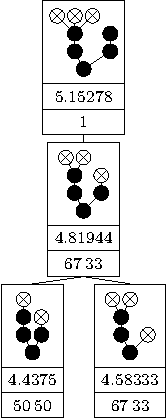
\includegraphics{p3/keep_3_busy/three_busy_opt.pdf}
    \caption{Optimal schedule. Keeps three processors busy for $7/9\approx 0.78$ time steps.}
  \end{subfigure}
  \quad
  \begin{subfigure}{.45\linewidth}
    \centering
    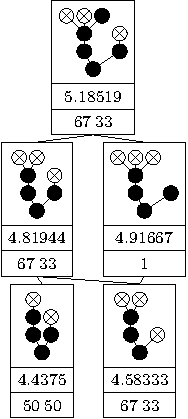
\includegraphics{p3/keep_3_busy/three_busy_subopt.pdf}
    \caption{This suboptimal schedule keeps three processors busy for expectedly $0.851852$ time steps.}
  \end{subfigure}
  \caption{An intree that shows that an optimal P3 schedule needs not keep busy three processors as long as possible. Snapshots with fewer than 6 tasks omitted since they have at most two tasks to be schedlued can be (optimally) processed via ordinary HLF. \todo{See figure \ref{fig:p3-p1s-suboptimal-example}!}}
  \label{fig:p3-p3l-suboptimal-example}
\end{figure}

Figure \ref{fig:p3-p1s-suboptimal-example} shows an intree with the property that the optimal schedule has an expected timespan of roughly 2.59259, within which only one processor is busy. On the other hand, a suboptimal schedule has a timespan of roughly 2.55555 within which only one processor is busy.

This shows that it can be useful to accept a longer time with only one processor busy, probably acchieving a longer time span where three processors are busy.

\begin{figure}[ht]
  \centering
  \renewcommand{\leveltopI}{-10cm + \leveltop}
\renewcommand{\leveltopII}{-10cm + \leveltopI}
\renewcommand{\leveltopIII}{-10cm + \leveltopII}
\renewcommand{\leveltopIIII}{-10cm + \leveltopIII}
\renewcommand{\leveltopIIIII}{-10cm + \leveltopIIII}
\renewcommand{\leveltopIIIIII}{-10cm + \leveltopIIIII}
\renewcommand{\leveltopIIIIIII}{-10cm + \leveltopIIIIII}
\begin{tikzpicture}[scale=.2, anchor=south]
\begin{scope}[yshift=\leveltopI cm]
\matrix (line1)[column sep=0.25cm] {
\node[draw=black, rectangle split,  rectangle split parts=2] (sn0x8a1c4d8){
\begin{tikzpicture}[scale=.2]
\node[circle, scale=0.75, fill] (tid0) at (3,1.5){};
\node[circle, scale=0.75, fill] (tid1) at (2.25,3){};
\node[circle, scale=0.75, fill, task_scheduled] (tid3) at (0.75,4.5){};
\node[circle, scale=0.75, fill, task_scheduled] (tid4) at (2.25,4.5){};
\node[circle, scale=0.75, fill, task_scheduled] (tid5) at (3.75,4.5){};
\draw[](tid1) -- (tid3);
\draw[](tid1) -- (tid4);
\draw[](tid1) -- (tid5);
\node[circle, scale=0.75, fill] (tid2) at (5.25,3){};
\node[circle, scale=0.75, fill] (tid6) at (5.25,4.5){};
\draw[](tid2) -- (tid6);
\draw[](tid0) -- (tid1);
\draw[](tid0) -- (tid2);
\end{tikzpicture}
\nodepart{two}
\footnotesize{$1$}
};
 & 
\\
};
\end{scope}
\begin{scope}[yshift=\leveltopII cm]
\matrix (line2)[column sep=0.25cm] {
\node[draw=black, rectangle split,  rectangle split parts=2] (sn0x8a1c3a0){
\begin{tikzpicture}[scale=.2]
\node[circle, scale=0.75, fill] (tid0) at (2.25,1.5){};
\node[circle, scale=0.75, fill] (tid1) at (1.5,3){};
\node[circle, scale=0.75, fill, task_scheduled] (tid3) at (0.75,4.5){};
\node[circle, scale=0.75, fill, task_scheduled] (tid4) at (2.25,4.5){};
\draw[](tid1) -- (tid3);
\draw[](tid1) -- (tid4);
\node[circle, scale=0.75, fill] (tid2) at (3.75,3){};
\node[circle, scale=0.75, fill, task_scheduled] (tid5) at (3.75,4.5){};
\draw[](tid2) -- (tid5);
\draw[](tid0) -- (tid1);
\draw[](tid0) -- (tid2);
\end{tikzpicture}
\nodepart{two}
\footnotesize{$33\:67$}
};
 & 
\\
};
\end{scope}
\begin{scope}[yshift=\leveltopIII cm]
\matrix (line3)[column sep=0.25cm] {
\node[draw=black, rectangle split,  rectangle split parts=2] (sn0x8a1bfc8){
\begin{tikzpicture}[scale=.2]
\node[circle, scale=0.75, fill] (tid0) at (2.25,1.5){};
\node[circle, scale=0.75, fill] (tid1) at (1.5,3){};
\node[circle, scale=0.75, fill, task_scheduled] (tid3) at (0.75,4.5){};
\node[circle, scale=0.75, fill, task_scheduled] (tid4) at (2.25,4.5){};
\draw[](tid1) -- (tid3);
\draw[](tid1) -- (tid4);
\node[circle, scale=0.75, fill, task_scheduled] (tid2) at (3.75,3){};
\draw[](tid0) -- (tid1);
\draw[](tid0) -- (tid2);
\end{tikzpicture}
\nodepart{two}
\footnotesize{$33\:67$}
};
 & 
\node[draw=black, rectangle split,  rectangle split parts=2] (sn0x8a1bcb8){
\begin{tikzpicture}[scale=.2]
\node[circle, scale=0.75, fill] (tid0) at (1.5,1.5){};
\node[circle, scale=0.75, fill] (tid1) at (0.75,3){};
\node[circle, scale=0.75, fill, task_scheduled] (tid3) at (0.75,4.5){};
\draw[](tid1) -- (tid3);
\node[circle, scale=0.75, fill] (tid2) at (2.25,3){};
\node[circle, scale=0.75, fill, task_scheduled] (tid4) at (2.25,4.5){};
\draw[](tid2) -- (tid4);
\draw[](tid0) -- (tid1);
\draw[](tid0) -- (tid2);
\end{tikzpicture}
\nodepart{two}
\footnotesize{$1$}
};
 & 
\\
};
\end{scope}
\begin{scope}[yshift=\leveltopIIII cm]
\matrix (line4)[column sep=0.25cm] {
\node[draw=black, rectangle split,  rectangle split parts=2] (sn0x8a1c238){
\begin{tikzpicture}[scale=.2]
\node[circle, scale=0.75, fill] (tid0) at (1.5,1.5){};
\node[circle, scale=0.75, fill] (tid1) at (1.5,3){};
\node[circle, scale=0.75, fill, task_scheduled] (tid2) at (0.75,4.5){};
\node[circle, scale=0.75, fill, task_scheduled] (tid3) at (2.25,4.5){};
\draw[](tid1) -- (tid2);
\draw[](tid1) -- (tid3);
\draw[](tid0) -- (tid1);
\end{tikzpicture}
\nodepart{two}
\footnotesize{$1$}
};
 & 
\node[draw=black, rectangle split,  rectangle split parts=2] (sn0x8a1bb98){
\begin{tikzpicture}[scale=.2]
\node[circle, scale=0.75, fill] (tid0) at (1.5,1.5){};
\node[circle, scale=0.75, fill] (tid1) at (0.75,3){};
\node[circle, scale=0.75, fill, task_scheduled] (tid3) at (0.75,4.5){};
\draw[](tid1) -- (tid3);
\node[circle, scale=0.75, fill, task_scheduled] (tid2) at (2.25,3){};
\draw[](tid0) -- (tid1);
\draw[](tid0) -- (tid2);
\end{tikzpicture}
\nodepart{two}
\footnotesize{$50\:50$}
};
 & 
\\
};
\end{scope}
\begin{scope}[yshift=\leveltopIIIII cm]
\matrix (line5)[column sep=0.25cm] {
\node[draw=black, rectangle split,  rectangle split parts=2] (sn0x8a1b940){
\begin{tikzpicture}[scale=.2]
\node[circle, scale=0.75, fill] (tid0) at (0.75,1.5){};
\node[circle, scale=0.75, fill] (tid1) at (0.75,3){};
\node[circle, scale=0.75, fill, task_scheduled] (tid2) at (0.75,4.5){};
\draw[](tid1) -- (tid2);
\draw[](tid0) -- (tid1);
\end{tikzpicture}
\nodepart{two}
\footnotesize{$1$}
};
 & 
\node[draw=black, rectangle split,  rectangle split parts=2] (sn0x8a1bb10){
\begin{tikzpicture}[scale=.2]
\node[circle, scale=0.75, fill] (tid0) at (1.5,1.5){};
\node[circle, scale=0.75, fill, task_scheduled] (tid1) at (0.75,3){};
\node[circle, scale=0.75, fill, task_scheduled] (tid2) at (2.25,3){};
\draw[](tid0) -- (tid1);
\draw[](tid0) -- (tid2);
\end{tikzpicture}
\nodepart{two}
\footnotesize{$1$}
};
 & 
\\
};
\end{scope}
\draw (sn0x8a1c4d8.south) -- (sn0x8a1c3a0.north);
\draw (sn0x8a1c3a0.south) -- (sn0x8a1bfc8.north);
\draw (sn0x8a1c3a0.south) -- (sn0x8a1bcb8.north);
\draw (sn0x8a1bfc8.south) -- (sn0x8a1c238.north);
\draw (sn0x8a1bfc8.south) -- (sn0x8a1bb98.north);
\draw (sn0x8a1bcb8.south) -- (sn0x8a1bb98.north);
\draw (sn0x8a1c238.south) -- (sn0x8a1b940.north);
\draw (sn0x8a1bb98.south) -- (sn0x8a1b940.north);
\draw (sn0x8a1bb98.south) -- (sn0x8a1bb10.north);
\end{tikzpicture}
\renewcommand{\leveltopI}{-10cm + \leveltop}
\renewcommand{\leveltopII}{-10cm + \leveltopI}
\renewcommand{\leveltopIII}{-10cm + \leveltopII}
\renewcommand{\leveltopIIII}{-10cm + \leveltopIII}
\renewcommand{\leveltopIIIII}{-10cm + \leveltopIIII}
\renewcommand{\leveltopIIIIII}{-10cm + \leveltopIIIII}
\renewcommand{\leveltopIIIIIII}{-10cm + \leveltopIIIIII}
\begin{tikzpicture}[scale=.2, anchor=south]
\begin{scope}[yshift=\leveltopI cm]
\matrix (line1)[column sep=0.25cm] {
\node[draw=black, rectangle split,  rectangle split parts=2] (sn0x8a1cdb8){
\begin{tikzpicture}[scale=.2]
\node[circle, scale=0.75, fill] (tid0) at (3,1.5){};
\node[circle, scale=0.75, fill] (tid1) at (2.25,3){};
\node[circle, scale=0.75, fill, task_scheduled] (tid3) at (0.75,4.5){};
\node[circle, scale=0.75, fill, task_scheduled] (tid4) at (2.25,4.5){};
\node[circle, scale=0.75, fill] (tid5) at (3.75,4.5){};
\draw[](tid1) -- (tid3);
\draw[](tid1) -- (tid4);
\draw[](tid1) -- (tid5);
\node[circle, scale=0.75, fill] (tid2) at (5.25,3){};
\node[circle, scale=0.75, fill, task_scheduled] (tid6) at (5.25,4.5){};
\draw[](tid2) -- (tid6);
\draw[](tid0) -- (tid1);
\draw[](tid0) -- (tid2);
\end{tikzpicture}
\nodepart{two}
\footnotesize{$33\:67$}
};
 & 
\\
};
\end{scope}
\begin{scope}[yshift=\leveltopII cm]
\matrix (line2)[column sep=0.25cm] {
\node[draw=black, rectangle split,  rectangle split parts=2] (sn0x8a1ca58){
\begin{tikzpicture}[scale=.2]
\node[circle, scale=0.75, fill] (tid0) at (3,1.5){};
\node[circle, scale=0.75, fill] (tid1) at (2.25,3){};
\node[circle, scale=0.75, fill, task_scheduled] (tid3) at (0.75,4.5){};
\node[circle, scale=0.75, fill, task_scheduled] (tid4) at (2.25,4.5){};
\node[circle, scale=0.75, fill, task_scheduled] (tid5) at (3.75,4.5){};
\draw[](tid1) -- (tid3);
\draw[](tid1) -- (tid4);
\draw[](tid1) -- (tid5);
\node[circle, scale=0.75, fill] (tid2) at (5.25,3){};
\draw[](tid0) -- (tid1);
\draw[](tid0) -- (tid2);
\end{tikzpicture}
\nodepart{two}
\footnotesize{$1$}
};
 & 
\node[draw=black, rectangle split,  rectangle split parts=2] (sn0x8a1c3a0){
\begin{tikzpicture}[scale=.2]
\node[circle, scale=0.75, fill] (tid0) at (2.25,1.5){};
\node[circle, scale=0.75, fill] (tid1) at (1.5,3){};
\node[circle, scale=0.75, fill, task_scheduled] (tid3) at (0.75,4.5){};
\node[circle, scale=0.75, fill, task_scheduled] (tid4) at (2.25,4.5){};
\draw[](tid1) -- (tid3);
\draw[](tid1) -- (tid4);
\node[circle, scale=0.75, fill] (tid2) at (3.75,3){};
\node[circle, scale=0.75, fill, task_scheduled] (tid5) at (3.75,4.5){};
\draw[](tid2) -- (tid5);
\draw[](tid0) -- (tid1);
\draw[](tid0) -- (tid2);
\end{tikzpicture}
\nodepart{two}
\footnotesize{$33\:67$}
};
 & 
\\
};
\end{scope}
\begin{scope}[yshift=\leveltopIII cm]
\matrix (line3)[column sep=0.25cm] {
\node[draw=black, rectangle split,  rectangle split parts=2] (sn0x8a1bfc8){
\begin{tikzpicture}[scale=.2]
\node[circle, scale=0.75, fill] (tid0) at (2.25,1.5){};
\node[circle, scale=0.75, fill] (tid1) at (1.5,3){};
\node[circle, scale=0.75, fill, task_scheduled] (tid3) at (0.75,4.5){};
\node[circle, scale=0.75, fill, task_scheduled] (tid4) at (2.25,4.5){};
\draw[](tid1) -- (tid3);
\draw[](tid1) -- (tid4);
\node[circle, scale=0.75, fill, task_scheduled] (tid2) at (3.75,3){};
\draw[](tid0) -- (tid1);
\draw[](tid0) -- (tid2);
\end{tikzpicture}
\nodepart{two}
\footnotesize{$33\:67$}
};
 & 
\node[draw=black, rectangle split,  rectangle split parts=2] (sn0x8a1bcb8){
\begin{tikzpicture}[scale=.2]
\node[circle, scale=0.75, fill] (tid0) at (1.5,1.5){};
\node[circle, scale=0.75, fill] (tid1) at (0.75,3){};
\node[circle, scale=0.75, fill, task_scheduled] (tid3) at (0.75,4.5){};
\draw[](tid1) -- (tid3);
\node[circle, scale=0.75, fill] (tid2) at (2.25,3){};
\node[circle, scale=0.75, fill, task_scheduled] (tid4) at (2.25,4.5){};
\draw[](tid2) -- (tid4);
\draw[](tid0) -- (tid1);
\draw[](tid0) -- (tid2);
\end{tikzpicture}
\nodepart{two}
\footnotesize{$1$}
};
 & 
\\
};
\end{scope}
\begin{scope}[yshift=\leveltopIIII cm]
\matrix (line4)[column sep=0.25cm] {
\node[draw=black, rectangle split,  rectangle split parts=2] (sn0x8a1c238){
\begin{tikzpicture}[scale=.2]
\node[circle, scale=0.75, fill] (tid0) at (1.5,1.5){};
\node[circle, scale=0.75, fill] (tid1) at (1.5,3){};
\node[circle, scale=0.75, fill, task_scheduled] (tid2) at (0.75,4.5){};
\node[circle, scale=0.75, fill, task_scheduled] (tid3) at (2.25,4.5){};
\draw[](tid1) -- (tid2);
\draw[](tid1) -- (tid3);
\draw[](tid0) -- (tid1);
\end{tikzpicture}
\nodepart{two}
\footnotesize{$1$}
};
 & 
\node[draw=black, rectangle split,  rectangle split parts=2] (sn0x8a1bb98){
\begin{tikzpicture}[scale=.2]
\node[circle, scale=0.75, fill] (tid0) at (1.5,1.5){};
\node[circle, scale=0.75, fill] (tid1) at (0.75,3){};
\node[circle, scale=0.75, fill, task_scheduled] (tid3) at (0.75,4.5){};
\draw[](tid1) -- (tid3);
\node[circle, scale=0.75, fill, task_scheduled] (tid2) at (2.25,3){};
\draw[](tid0) -- (tid1);
\draw[](tid0) -- (tid2);
\end{tikzpicture}
\nodepart{two}
\footnotesize{$50\:50$}
};
 & 
\\
};
\end{scope}
\begin{scope}[yshift=\leveltopIIIII cm]
\matrix (line5)[column sep=0.25cm] {
\node[draw=black, rectangle split,  rectangle split parts=2] (sn0x8a1b940){
\begin{tikzpicture}[scale=.2]
\node[circle, scale=0.75, fill] (tid0) at (0.75,1.5){};
\node[circle, scale=0.75, fill] (tid1) at (0.75,3){};
\node[circle, scale=0.75, fill, task_scheduled] (tid2) at (0.75,4.5){};
\draw[](tid1) -- (tid2);
\draw[](tid0) -- (tid1);
\end{tikzpicture}
\nodepart{two}
\footnotesize{$1$}
};
 & 
\node[draw=black, rectangle split,  rectangle split parts=2] (sn0x8a1bb10){
\begin{tikzpicture}[scale=.2]
\node[circle, scale=0.75, fill] (tid0) at (1.5,1.5){};
\node[circle, scale=0.75, fill, task_scheduled] (tid1) at (0.75,3){};
\node[circle, scale=0.75, fill, task_scheduled] (tid2) at (2.25,3){};
\draw[](tid0) -- (tid1);
\draw[](tid0) -- (tid2);
\end{tikzpicture}
\nodepart{two}
\footnotesize{$1$}
};
 & 
\\
};
\end{scope}
\draw (sn0x8a1cdb8.south) -- (sn0x8a1ca58.north);
\draw (sn0x8a1cdb8.south) -- (sn0x8a1c3a0.north);
\draw (sn0x8a1ca58.south) -- (sn0x8a1bfc8.north);
\draw (sn0x8a1c3a0.south) -- (sn0x8a1bfc8.north);
\draw (sn0x8a1c3a0.south) -- (sn0x8a1bcb8.north);
\draw (sn0x8a1bfc8.south) -- (sn0x8a1c238.north);
\draw (sn0x8a1bfc8.south) -- (sn0x8a1bb98.north);
\draw (sn0x8a1bcb8.south) -- (sn0x8a1bb98.north);
\draw (sn0x8a1c238.south) -- (sn0x8a1b940.north);
\draw (sn0x8a1bb98.south) -- (sn0x8a1b940.north);
\draw (sn0x8a1bb98.south) -- (sn0x8a1bb10.north);
\end{tikzpicture}

%%% Local Variables:
%%% TeX-master: "thesis/thesis.tex"
%%% End: 

  \caption{An intree where the expected time with only one processor being busy is longer within the optimal schedule ($\approx 2.59259$) than within a suboptimal schedule ($\approx 2.555555$).\todo{Write expected times which only one busy processor in subfigures.} \todo{Convert to fractions.}\todo{Which one is optimal? Subfigures!}}
  \label{fig:p3-p1s-suboptimal-example}
\end{figure}

It can also be shown that even combining the two arguments -- in the sense that P3L \emph{or} P1S should be fulfilled for the optimal schedule -- is not correct. This can be observed by examining the intree $(0, 0, 1, 1, 2, 3, 3, 3)$. Figure \ref{fig:p3l-p1s-combo-suboptimal} shows this example.

\begin{figure}[ht]
  \centering
  \renewcommand{\leveltopI}{-10cm + \leveltop}
\renewcommand{\leveltopII}{-10cm + \leveltopI}
\renewcommand{\leveltopIII}{-10cm + \leveltopII}
\renewcommand{\leveltopIIII}{-10cm + \leveltopIII}
\renewcommand{\leveltopIIIII}{-10cm + \leveltopIIII}
\renewcommand{\leveltopIIIIII}{-10cm + \leveltopIIIII}
\renewcommand{\leveltopIIIIIII}{-10cm + \leveltopIIIIII}
\renewcommand{\leveltopIIIIIIII}{-10cm + \leveltopIIIIIII}
\renewcommand{\leveltopIIIIIIIII}{-10cm + \leveltopIIIIIIII}
\begin{tikzpicture}[scale=.2, anchor=south]
\begin{scope}[yshift=\leveltopI cm]
\matrix (line1)[column sep=0.25cm] {
\node[draw=black, rectangle split,  rectangle split parts=2] (sn0x9940640){
\begin{tikzpicture}[scale=.2]
\node[circle, scale=0.75, fill] (tid0) at (3.75,1.5){};
\node[circle, scale=0.75, fill] (tid1) at (3,3){};
\node[circle, scale=0.75, fill] (tid3) at (2.25,4.5){};
\node[circle, scale=0.75, fill, task_scheduled] (tid6) at (0.75,6){};
\node[circle, scale=0.75, fill, task_scheduled] (tid7) at (2.25,6){};
\node[circle, scale=0.75, fill] (tid8) at (3.75,6){};
\draw[](tid3) -- (tid6);
\draw[](tid3) -- (tid7);
\draw[](tid3) -- (tid8);
\node[circle, scale=0.75, fill, task_scheduled] (tid4) at (5.25,4.5){};
\draw[](tid1) -- (tid3);
\draw[](tid1) -- (tid4);
\node[circle, scale=0.75, fill] (tid2) at (6.75,3){};
\node[circle, scale=0.75, fill] (tid5) at (6.75,4.5){};
\draw[](tid2) -- (tid5);
\draw[](tid0) -- (tid1);
\draw[](tid0) -- (tid2);
\end{tikzpicture}
\nodepart{two}
\footnotesize{$33\:67$}
};
 & 
\\
};
\end{scope}
\begin{scope}[yshift=\leveltopII cm]
\matrix (line2)[column sep=0.25cm] {
\node[draw=black, rectangle split,  rectangle split parts=2] (sn0x993e580){
\begin{tikzpicture}[scale=.2]
\node[circle, scale=0.75, fill] (tid0) at (3,1.5){};
\node[circle, scale=0.75, fill] (tid1) at (2.25,3){};
\node[circle, scale=0.75, fill] (tid3) at (2.25,4.5){};
\node[circle, scale=0.75, fill, task_scheduled] (tid5) at (0.75,6){};
\node[circle, scale=0.75, fill, task_scheduled] (tid6) at (2.25,6){};
\node[circle, scale=0.75, fill, task_scheduled] (tid7) at (3.75,6){};
\draw[](tid3) -- (tid5);
\draw[](tid3) -- (tid6);
\draw[](tid3) -- (tid7);
\draw[](tid1) -- (tid3);
\node[circle, scale=0.75, fill] (tid2) at (5.25,3){};
\node[circle, scale=0.75, fill] (tid4) at (5.25,4.5){};
\draw[](tid2) -- (tid4);
\draw[](tid0) -- (tid1);
\draw[](tid0) -- (tid2);
\end{tikzpicture}
\nodepart{two}
\footnotesize{$1$}
};
 & 
\node[draw=black, rectangle split,  rectangle split parts=2] (sn0x9940918){
\begin{tikzpicture}[scale=.2]
\node[circle, scale=0.75, fill] (tid0) at (3,1.5){};
\node[circle, scale=0.75, fill] (tid1) at (2.25,3){};
\node[circle, scale=0.75, fill] (tid3) at (1.5,4.5){};
\node[circle, scale=0.75, fill, task_scheduled] (tid6) at (0.75,6){};
\node[circle, scale=0.75, fill, task_scheduled] (tid7) at (2.25,6){};
\draw[](tid3) -- (tid6);
\draw[](tid3) -- (tid7);
\node[circle, scale=0.75, fill, task_scheduled] (tid4) at (3.75,4.5){};
\draw[](tid1) -- (tid3);
\draw[](tid1) -- (tid4);
\node[circle, scale=0.75, fill] (tid2) at (5.25,3){};
\node[circle, scale=0.75, fill] (tid5) at (5.25,4.5){};
\draw[](tid2) -- (tid5);
\draw[](tid0) -- (tid1);
\draw[](tid0) -- (tid2);
\end{tikzpicture}
\nodepart{two}
\footnotesize{$33\:67$}
};
 & 
\\
};
\end{scope}
\begin{scope}[yshift=\leveltopIII cm]
\matrix (line3)[column sep=0.25cm] {
\node[draw=black, rectangle split,  rectangle split parts=2] (sn0x993e438){
\begin{tikzpicture}[scale=.2]
\node[circle, scale=0.75, fill] (tid0) at (2.25,1.5){};
\node[circle, scale=0.75, fill] (tid1) at (1.5,3){};
\node[circle, scale=0.75, fill] (tid3) at (1.5,4.5){};
\node[circle, scale=0.75, fill, task_scheduled] (tid5) at (0.75,6){};
\node[circle, scale=0.75, fill, task_scheduled] (tid6) at (2.25,6){};
\draw[](tid3) -- (tid5);
\draw[](tid3) -- (tid6);
\draw[](tid1) -- (tid3);
\node[circle, scale=0.75, fill] (tid2) at (3.75,3){};
\node[circle, scale=0.75, fill, task_scheduled] (tid4) at (3.75,4.5){};
\draw[](tid2) -- (tid4);
\draw[](tid0) -- (tid1);
\draw[](tid0) -- (tid2);
\end{tikzpicture}
\nodepart{two}
\footnotesize{$33\:67$}
};
 & 
\node[draw=black, rectangle split,  rectangle split parts=2] (sn0x9940378){
\begin{tikzpicture}[scale=.2]
\node[circle, scale=0.75, fill] (tid0) at (2.25,1.5){};
\node[circle, scale=0.75, fill] (tid1) at (1.5,3){};
\node[circle, scale=0.75, fill] (tid3) at (0.75,4.5){};
\node[circle, scale=0.75, fill, task_scheduled] (tid6) at (0.75,6){};
\draw[](tid3) -- (tid6);
\node[circle, scale=0.75, fill, task_scheduled] (tid4) at (2.25,4.5){};
\draw[](tid1) -- (tid3);
\draw[](tid1) -- (tid4);
\node[circle, scale=0.75, fill] (tid2) at (3.75,3){};
\node[circle, scale=0.75, fill, task_scheduled] (tid5) at (3.75,4.5){};
\draw[](tid2) -- (tid5);
\draw[](tid0) -- (tid1);
\draw[](tid0) -- (tid2);
\end{tikzpicture}
\nodepart{two}
\footnotesize{$33\:33\:33$}
};
 & 
\\
};
\end{scope}
\begin{scope}[yshift=\leveltopIIII cm]
\matrix (line4)[column sep=0.25cm] {
\node[draw=black, rectangle split,  rectangle split parts=2] (sn0x993d988){
\begin{tikzpicture}[scale=.2]
\node[circle, scale=0.75, fill] (tid0) at (2.25,1.5){};
\node[circle, scale=0.75, fill] (tid1) at (1.5,3){};
\node[circle, scale=0.75, fill] (tid3) at (1.5,4.5){};
\node[circle, scale=0.75, fill, task_scheduled] (tid4) at (0.75,6){};
\node[circle, scale=0.75, fill, task_scheduled] (tid5) at (2.25,6){};
\draw[](tid3) -- (tid4);
\draw[](tid3) -- (tid5);
\draw[](tid1) -- (tid3);
\node[circle, scale=0.75, fill, task_scheduled] (tid2) at (3.75,3){};
\draw[](tid0) -- (tid1);
\draw[](tid0) -- (tid2);
\end{tikzpicture}
\nodepart{two}
\footnotesize{$33\:67$}
};
 & 
\node[draw=black, rectangle split,  rectangle split parts=2] (sn0x993f700){
\begin{tikzpicture}[scale=.2]
\node[circle, scale=0.75, fill] (tid0) at (2.25,1.5){};
\node[circle, scale=0.75, fill] (tid1) at (1.5,3){};
\node[circle, scale=0.75, fill] (tid3) at (0.75,4.5){};
\node[circle, scale=0.75, fill, task_scheduled] (tid5) at (0.75,6){};
\draw[](tid3) -- (tid5);
\node[circle, scale=0.75, fill, task_scheduled] (tid4) at (2.25,4.5){};
\draw[](tid1) -- (tid3);
\draw[](tid1) -- (tid4);
\node[circle, scale=0.75, fill, task_scheduled] (tid2) at (3.75,3){};
\draw[](tid0) -- (tid1);
\draw[](tid0) -- (tid2);
\end{tikzpicture}
\nodepart{two}
\footnotesize{$33\:33\:33$}
};
 & 
\node[draw=black, rectangle split,  rectangle split parts=2] (sn0x993e010){
\begin{tikzpicture}[scale=.2]
\node[circle, scale=0.75, fill] (tid0) at (1.5,1.5){};
\node[circle, scale=0.75, fill] (tid1) at (0.75,3){};
\node[circle, scale=0.75, fill] (tid3) at (0.75,4.5){};
\node[circle, scale=0.75, fill, task_scheduled] (tid5) at (0.75,6){};
\draw[](tid3) -- (tid5);
\draw[](tid1) -- (tid3);
\node[circle, scale=0.75, fill] (tid2) at (2.25,3){};
\node[circle, scale=0.75, fill, task_scheduled] (tid4) at (2.25,4.5){};
\draw[](tid2) -- (tid4);
\draw[](tid0) -- (tid1);
\draw[](tid0) -- (tid2);
\end{tikzpicture}
\nodepart{two}
\footnotesize{$50\:50$}
};
 & 
\node[draw=black, rectangle split,  rectangle split parts=2] (sn0x9940050){
\begin{tikzpicture}[scale=.2]
\node[circle, scale=0.75, fill] (tid0) at (2.25,1.5){};
\node[circle, scale=0.75, fill] (tid1) at (1.5,3){};
\node[circle, scale=0.75, fill, task_scheduled] (tid3) at (0.75,4.5){};
\node[circle, scale=0.75, fill, task_scheduled] (tid4) at (2.25,4.5){};
\draw[](tid1) -- (tid3);
\draw[](tid1) -- (tid4);
\node[circle, scale=0.75, fill] (tid2) at (3.75,3){};
\node[circle, scale=0.75, fill, task_scheduled] (tid5) at (3.75,4.5){};
\draw[](tid2) -- (tid5);
\draw[](tid0) -- (tid1);
\draw[](tid0) -- (tid2);
\end{tikzpicture}
\nodepart{two}
\footnotesize{$67\:33$}
};
 & 
\\
};
\end{scope}
\draw (sn0x9940640.south) -- (sn0x993e580.north);
\draw (sn0x9940640.south) -- (sn0x9940918.north);
\draw (sn0x993e580.south) -- (sn0x993e438.north);
\draw (sn0x9940918.south) -- (sn0x993e438.north);
\draw (sn0x9940918.south) -- (sn0x9940378.north);
\draw (sn0x993e438.south) -- (sn0x993d988.north);
\draw (sn0x993e438.south) -- (sn0x993e010.north);
\draw (sn0x9940378.south) -- (sn0x993f700.north);
\draw (sn0x9940378.south) -- (sn0x993e010.north);
\draw (sn0x9940378.south) -- (sn0x9940050.north);
\end{tikzpicture}
\renewcommand{\leveltopI}{-10cm + \leveltop}
\renewcommand{\leveltopII}{-10cm + \leveltopI}
\renewcommand{\leveltopIII}{-10cm + \leveltopII}
\renewcommand{\leveltopIIII}{-10cm + \leveltopIII}
\renewcommand{\leveltopIIIII}{-10cm + \leveltopIIII}
\renewcommand{\leveltopIIIIII}{-10cm + \leveltopIIIII}
\renewcommand{\leveltopIIIIIII}{-10cm + \leveltopIIIIII}
\renewcommand{\leveltopIIIIIIII}{-10cm + \leveltopIIIIIII}
\renewcommand{\leveltopIIIIIIIII}{-10cm + \leveltopIIIIIIII}
\begin{tikzpicture}[scale=.2, anchor=south]
\begin{scope}[yshift=\leveltopI cm]
\matrix (line1)[column sep=0.25cm] {
\node[draw=black, rectangle split,  rectangle split parts=2] (sn0x9941330){
\begin{tikzpicture}[scale=.2]
\node[circle, scale=0.75, fill] (tid0) at (3.75,1.5){};
\node[circle, scale=0.75, fill] (tid1) at (3,3){};
\node[circle, scale=0.75, fill] (tid3) at (2.25,4.5){};
\node[circle, scale=0.75, fill, task_scheduled] (tid6) at (0.75,6){};
\node[circle, scale=0.75, fill] (tid7) at (2.25,6){};
\node[circle, scale=0.75, fill] (tid8) at (3.75,6){};
\draw[](tid3) -- (tid6);
\draw[](tid3) -- (tid7);
\draw[](tid3) -- (tid8);
\node[circle, scale=0.75, fill, task_scheduled] (tid4) at (5.25,4.5){};
\draw[](tid1) -- (tid3);
\draw[](tid1) -- (tid4);
\node[circle, scale=0.75, fill] (tid2) at (6.75,3){};
\node[circle, scale=0.75, fill, task_scheduled] (tid5) at (6.75,4.5){};
\draw[](tid2) -- (tid5);
\draw[](tid0) -- (tid1);
\draw[](tid0) -- (tid2);
\end{tikzpicture}
\nodepart{two}
\footnotesize{$33\:33\:33$}
};
 & 
\\
};
\end{scope}
\begin{scope}[yshift=\leveltopII cm]
\matrix (line2)[column sep=0.25cm] {
\node[draw=black, rectangle split,  rectangle split parts=2] (sn0x99416c8){
\begin{tikzpicture}[scale=.2]
\node[circle, scale=0.75, fill] (tid0) at (3.75,1.5){};
\node[circle, scale=0.75, fill] (tid1) at (3,3){};
\node[circle, scale=0.75, fill] (tid3) at (2.25,4.5){};
\node[circle, scale=0.75, fill, task_scheduled] (tid5) at (0.75,6){};
\node[circle, scale=0.75, fill, task_scheduled] (tid6) at (2.25,6){};
\node[circle, scale=0.75, fill] (tid7) at (3.75,6){};
\draw[](tid3) -- (tid5);
\draw[](tid3) -- (tid6);
\draw[](tid3) -- (tid7);
\node[circle, scale=0.75, fill, task_scheduled] (tid4) at (5.25,4.5){};
\draw[](tid1) -- (tid3);
\draw[](tid1) -- (tid4);
\node[circle, scale=0.75, fill] (tid2) at (6.75,3){};
\draw[](tid0) -- (tid1);
\draw[](tid0) -- (tid2);
\end{tikzpicture}
\nodepart{two}
\footnotesize{$33\:67$}
};
 & 
\node[draw=black, rectangle split,  rectangle split parts=2] (sn0x993e518){
\begin{tikzpicture}[scale=.2]
\node[circle, scale=0.75, fill] (tid0) at (3,1.5){};
\node[circle, scale=0.75, fill] (tid1) at (2.25,3){};
\node[circle, scale=0.75, fill] (tid3) at (2.25,4.5){};
\node[circle, scale=0.75, fill, task_scheduled] (tid5) at (0.75,6){};
\node[circle, scale=0.75, fill, task_scheduled] (tid6) at (2.25,6){};
\node[circle, scale=0.75, fill] (tid7) at (3.75,6){};
\draw[](tid3) -- (tid5);
\draw[](tid3) -- (tid6);
\draw[](tid3) -- (tid7);
\draw[](tid1) -- (tid3);
\node[circle, scale=0.75, fill] (tid2) at (5.25,3){};
\node[circle, scale=0.75, fill, task_scheduled] (tid4) at (5.25,4.5){};
\draw[](tid2) -- (tid4);
\draw[](tid0) -- (tid1);
\draw[](tid0) -- (tid2);
\end{tikzpicture}
\nodepart{two}
\footnotesize{$33\:67$}
};
 & 
\node[draw=black, rectangle split,  rectangle split parts=2] (sn0x99403e0){
\begin{tikzpicture}[scale=.2]
\node[circle, scale=0.75, fill] (tid0) at (3,1.5){};
\node[circle, scale=0.75, fill] (tid1) at (2.25,3){};
\node[circle, scale=0.75, fill] (tid3) at (1.5,4.5){};
\node[circle, scale=0.75, fill, task_scheduled] (tid6) at (0.75,6){};
\node[circle, scale=0.75, fill] (tid7) at (2.25,6){};
\draw[](tid3) -- (tid6);
\draw[](tid3) -- (tid7);
\node[circle, scale=0.75, fill, task_scheduled] (tid4) at (3.75,4.5){};
\draw[](tid1) -- (tid3);
\draw[](tid1) -- (tid4);
\node[circle, scale=0.75, fill] (tid2) at (5.25,3){};
\node[circle, scale=0.75, fill, task_scheduled] (tid5) at (5.25,4.5){};
\draw[](tid2) -- (tid5);
\draw[](tid0) -- (tid1);
\draw[](tid0) -- (tid2);
\end{tikzpicture}
\nodepart{two}
\footnotesize{$33\:33\:33$}
};
 & 
\\
};
\end{scope}
\begin{scope}[yshift=\leveltopIII cm]
\matrix (line3)[column sep=0.25cm] {
\node[draw=black, rectangle split,  rectangle split parts=2] (sn0x993d8b8){
\begin{tikzpicture}[scale=.2]
\node[circle, scale=0.75, fill] (tid0) at (3,1.5){};
\node[circle, scale=0.75, fill] (tid1) at (2.25,3){};
\node[circle, scale=0.75, fill] (tid3) at (2.25,4.5){};
\node[circle, scale=0.75, fill, task_scheduled] (tid4) at (0.75,6){};
\node[circle, scale=0.75, fill, task_scheduled] (tid5) at (2.25,6){};
\node[circle, scale=0.75, fill, task_scheduled] (tid6) at (3.75,6){};
\draw[](tid3) -- (tid4);
\draw[](tid3) -- (tid5);
\draw[](tid3) -- (tid6);
\draw[](tid1) -- (tid3);
\node[circle, scale=0.75, fill] (tid2) at (5.25,3){};
\draw[](tid0) -- (tid1);
\draw[](tid0) -- (tid2);
\end{tikzpicture}
\nodepart{two}
\footnotesize{$1$}
};
 & 
\node[draw=black, rectangle split,  rectangle split parts=2] (sn0x993fb10){
\begin{tikzpicture}[scale=.2]
\node[circle, scale=0.75, fill] (tid0) at (3,1.5){};
\node[circle, scale=0.75, fill] (tid1) at (2.25,3){};
\node[circle, scale=0.75, fill] (tid3) at (1.5,4.5){};
\node[circle, scale=0.75, fill, task_scheduled] (tid5) at (0.75,6){};
\node[circle, scale=0.75, fill, task_scheduled] (tid6) at (2.25,6){};
\draw[](tid3) -- (tid5);
\draw[](tid3) -- (tid6);
\node[circle, scale=0.75, fill, task_scheduled] (tid4) at (3.75,4.5){};
\draw[](tid1) -- (tid3);
\draw[](tid1) -- (tid4);
\node[circle, scale=0.75, fill] (tid2) at (5.25,3){};
\draw[](tid0) -- (tid1);
\draw[](tid0) -- (tid2);
\end{tikzpicture}
\nodepart{two}
\footnotesize{$33\:67$}
};
 & 
\node[draw=black, rectangle split,  rectangle split parts=2] (sn0x993e438){
\begin{tikzpicture}[scale=.2]
\node[circle, scale=0.75, fill] (tid0) at (2.25,1.5){};
\node[circle, scale=0.75, fill] (tid1) at (1.5,3){};
\node[circle, scale=0.75, fill] (tid3) at (1.5,4.5){};
\node[circle, scale=0.75, fill, task_scheduled] (tid5) at (0.75,6){};
\node[circle, scale=0.75, fill, task_scheduled] (tid6) at (2.25,6){};
\draw[](tid3) -- (tid5);
\draw[](tid3) -- (tid6);
\draw[](tid1) -- (tid3);
\node[circle, scale=0.75, fill] (tid2) at (3.75,3){};
\node[circle, scale=0.75, fill, task_scheduled] (tid4) at (3.75,4.5){};
\draw[](tid2) -- (tid4);
\draw[](tid0) -- (tid1);
\draw[](tid0) -- (tid2);
\end{tikzpicture}
\nodepart{two}
\footnotesize{$33\:67$}
};
 & 
\node[draw=black, rectangle split,  rectangle split parts=2] (sn0x9940378){
\begin{tikzpicture}[scale=.2]
\node[circle, scale=0.75, fill] (tid0) at (2.25,1.5){};
\node[circle, scale=0.75, fill] (tid1) at (1.5,3){};
\node[circle, scale=0.75, fill] (tid3) at (0.75,4.5){};
\node[circle, scale=0.75, fill, task_scheduled] (tid6) at (0.75,6){};
\draw[](tid3) -- (tid6);
\node[circle, scale=0.75, fill, task_scheduled] (tid4) at (2.25,4.5){};
\draw[](tid1) -- (tid3);
\draw[](tid1) -- (tid4);
\node[circle, scale=0.75, fill] (tid2) at (3.75,3){};
\node[circle, scale=0.75, fill, task_scheduled] (tid5) at (3.75,4.5){};
\draw[](tid2) -- (tid5);
\draw[](tid0) -- (tid1);
\draw[](tid0) -- (tid2);
\end{tikzpicture}
\nodepart{two}
\footnotesize{$33\:33\:33$}
};
 & 
\\
};
\end{scope}
\begin{scope}[yshift=\leveltopIIII cm]
\matrix (line4)[column sep=0.25cm] {
\node[draw=black, rectangle split,  rectangle split parts=2] (sn0x993d988){
\begin{tikzpicture}[scale=.2]
\node[circle, scale=0.75, fill] (tid0) at (2.25,1.5){};
\node[circle, scale=0.75, fill] (tid1) at (1.5,3){};
\node[circle, scale=0.75, fill] (tid3) at (1.5,4.5){};
\node[circle, scale=0.75, fill, task_scheduled] (tid4) at (0.75,6){};
\node[circle, scale=0.75, fill, task_scheduled] (tid5) at (2.25,6){};
\draw[](tid3) -- (tid4);
\draw[](tid3) -- (tid5);
\draw[](tid1) -- (tid3);
\node[circle, scale=0.75, fill, task_scheduled] (tid2) at (3.75,3){};
\draw[](tid0) -- (tid1);
\draw[](tid0) -- (tid2);
\end{tikzpicture}
\nodepart{two}
\footnotesize{$33\:67$}
};
 & 
\node[draw=black, rectangle split,  rectangle split parts=2] (sn0x993f700){
\begin{tikzpicture}[scale=.2]
\node[circle, scale=0.75, fill] (tid0) at (2.25,1.5){};
\node[circle, scale=0.75, fill] (tid1) at (1.5,3){};
\node[circle, scale=0.75, fill] (tid3) at (0.75,4.5){};
\node[circle, scale=0.75, fill, task_scheduled] (tid5) at (0.75,6){};
\draw[](tid3) -- (tid5);
\node[circle, scale=0.75, fill, task_scheduled] (tid4) at (2.25,4.5){};
\draw[](tid1) -- (tid3);
\draw[](tid1) -- (tid4);
\node[circle, scale=0.75, fill, task_scheduled] (tid2) at (3.75,3){};
\draw[](tid0) -- (tid1);
\draw[](tid0) -- (tid2);
\end{tikzpicture}
\nodepart{two}
\footnotesize{$33\:33\:33$}
};
 & 
\node[draw=black, rectangle split,  rectangle split parts=2] (sn0x993e010){
\begin{tikzpicture}[scale=.2]
\node[circle, scale=0.75, fill] (tid0) at (1.5,1.5){};
\node[circle, scale=0.75, fill] (tid1) at (0.75,3){};
\node[circle, scale=0.75, fill] (tid3) at (0.75,4.5){};
\node[circle, scale=0.75, fill, task_scheduled] (tid5) at (0.75,6){};
\draw[](tid3) -- (tid5);
\draw[](tid1) -- (tid3);
\node[circle, scale=0.75, fill] (tid2) at (2.25,3){};
\node[circle, scale=0.75, fill, task_scheduled] (tid4) at (2.25,4.5){};
\draw[](tid2) -- (tid4);
\draw[](tid0) -- (tid1);
\draw[](tid0) -- (tid2);
\end{tikzpicture}
\nodepart{two}
\footnotesize{$50\:50$}
};
 & 
\node[draw=black, rectangle split,  rectangle split parts=2] (sn0x9940050){
\begin{tikzpicture}[scale=.2]
\node[circle, scale=0.75, fill] (tid0) at (2.25,1.5){};
\node[circle, scale=0.75, fill] (tid1) at (1.5,3){};
\node[circle, scale=0.75, fill, task_scheduled] (tid3) at (0.75,4.5){};
\node[circle, scale=0.75, fill, task_scheduled] (tid4) at (2.25,4.5){};
\draw[](tid1) -- (tid3);
\draw[](tid1) -- (tid4);
\node[circle, scale=0.75, fill] (tid2) at (3.75,3){};
\node[circle, scale=0.75, fill, task_scheduled] (tid5) at (3.75,4.5){};
\draw[](tid2) -- (tid5);
\draw[](tid0) -- (tid1);
\draw[](tid0) -- (tid2);
\end{tikzpicture}
\nodepart{two}
\footnotesize{$33\:67$}
};
 & 
\\
};
\end{scope}
\draw (sn0x9941330.south) -- (sn0x99416c8.north);
\draw (sn0x9941330.south) -- (sn0x993e518.north);
\draw (sn0x9941330.south) -- (sn0x99403e0.north);
\draw (sn0x99416c8.south) -- (sn0x993d8b8.north);
\draw (sn0x99416c8.south) -- (sn0x993fb10.north);
\draw (sn0x993e518.south) -- (sn0x993d8b8.north);
\draw (sn0x993e518.south) -- (sn0x993e438.north);
\draw (sn0x99403e0.south) -- (sn0x993fb10.north);
\draw (sn0x99403e0.south) -- (sn0x993e438.north);
\draw (sn0x99403e0.south) -- (sn0x9940378.north);
\draw (sn0x993d8b8.south) -- (sn0x993d988.north);
\draw (sn0x993fb10.south) -- (sn0x993d988.north);
\draw (sn0x993fb10.south) -- (sn0x993f700.north);
\draw (sn0x993e438.south) -- (sn0x993d988.north);
\draw (sn0x993e438.south) -- (sn0x993e010.north);
\draw (sn0x9940378.south) -- (sn0x993f700.north);
\draw (sn0x9940378.south) -- (sn0x993e010.north);
\draw (sn0x9940378.south) -- (sn0x9940050.north);
\end{tikzpicture}
\renewcommand{\leveltopI}{-10cm + \leveltop}
\renewcommand{\leveltopII}{-10cm + \leveltopI}
\renewcommand{\leveltopIII}{-10cm + \leveltopII}
\renewcommand{\leveltopIIII}{-10cm + \leveltopIII}
\renewcommand{\leveltopIIIII}{-10cm + \leveltopIIII}
\renewcommand{\leveltopIIIIII}{-10cm + \leveltopIIIII}
\renewcommand{\leveltopIIIIIII}{-10cm + \leveltopIIIIII}
\renewcommand{\leveltopIIIIIIII}{-10cm + \leveltopIIIIIII}
\renewcommand{\leveltopIIIIIIIII}{-10cm + \leveltopIIIIIIII}
\begin{tikzpicture}[scale=.2, anchor=south]
\begin{scope}[yshift=\leveltopI cm]
\matrix (line1)[column sep=0.25cm] {
\node[draw=black, rectangle split,  rectangle split parts=2] (sn0x99428e0){
\begin{tikzpicture}[scale=.2]
\node[circle, scale=0.75, fill] (tid0) at (3.75,1.5){};
\node[circle, scale=0.75, fill] (tid1) at (3,3){};
\node[circle, scale=0.75, fill] (tid3) at (2.25,4.5){};
\node[circle, scale=0.75, fill, task_scheduled] (tid6) at (0.75,6){};
\node[circle, scale=0.75, fill, task_scheduled] (tid7) at (2.25,6){};
\node[circle, scale=0.75, fill] (tid8) at (3.75,6){};
\draw[](tid3) -- (tid6);
\draw[](tid3) -- (tid7);
\draw[](tid3) -- (tid8);
\node[circle, scale=0.75, fill] (tid4) at (5.25,4.5){};
\draw[](tid1) -- (tid3);
\draw[](tid1) -- (tid4);
\node[circle, scale=0.75, fill] (tid2) at (6.75,3){};
\node[circle, scale=0.75, fill, task_scheduled] (tid5) at (6.75,4.5){};
\draw[](tid2) -- (tid5);
\draw[](tid0) -- (tid1);
\draw[](tid0) -- (tid2);
\end{tikzpicture}
\nodepart{two}
\footnotesize{$33\:67$}
};
 & 
\\
};
\end{scope}
\begin{scope}[yshift=\leveltopII cm]
\matrix (line2)[column sep=0.25cm] {
\node[draw=black, rectangle split,  rectangle split parts=2] (sn0x99417c8){
\begin{tikzpicture}[scale=.2]
\node[circle, scale=0.75, fill] (tid0) at (3.75,1.5){};
\node[circle, scale=0.75, fill] (tid1) at (3,3){};
\node[circle, scale=0.75, fill] (tid3) at (2.25,4.5){};
\node[circle, scale=0.75, fill, task_scheduled] (tid5) at (0.75,6){};
\node[circle, scale=0.75, fill, task_scheduled] (tid6) at (2.25,6){};
\node[circle, scale=0.75, fill, task_scheduled] (tid7) at (3.75,6){};
\draw[](tid3) -- (tid5);
\draw[](tid3) -- (tid6);
\draw[](tid3) -- (tid7);
\node[circle, scale=0.75, fill] (tid4) at (5.25,4.5){};
\draw[](tid1) -- (tid3);
\draw[](tid1) -- (tid4);
\node[circle, scale=0.75, fill] (tid2) at (6.75,3){};
\draw[](tid0) -- (tid1);
\draw[](tid0) -- (tid2);
\end{tikzpicture}
\nodepart{two}
\footnotesize{$1$}
};
 & 
\node[draw=black, rectangle split,  rectangle split parts=2] (sn0x9942878){
\begin{tikzpicture}[scale=.2]
\node[circle, scale=0.75, fill] (tid0) at (3,1.5){};
\node[circle, scale=0.75, fill] (tid1) at (2.25,3){};
\node[circle, scale=0.75, fill] (tid3) at (1.5,4.5){};
\node[circle, scale=0.75, fill, task_scheduled] (tid6) at (0.75,6){};
\node[circle, scale=0.75, fill, task_scheduled] (tid7) at (2.25,6){};
\draw[](tid3) -- (tid6);
\draw[](tid3) -- (tid7);
\node[circle, scale=0.75, fill] (tid4) at (3.75,4.5){};
\draw[](tid1) -- (tid3);
\draw[](tid1) -- (tid4);
\node[circle, scale=0.75, fill] (tid2) at (5.25,3){};
\node[circle, scale=0.75, fill, task_scheduled] (tid5) at (5.25,4.5){};
\draw[](tid2) -- (tid5);
\draw[](tid0) -- (tid1);
\draw[](tid0) -- (tid2);
\end{tikzpicture}
\nodepart{two}
\footnotesize{$33\:67$}
};
 & 
\\
};
\end{scope}
\begin{scope}[yshift=\leveltopIII cm]
\matrix (line3)[column sep=0.25cm] {
\node[draw=black, rectangle split,  rectangle split parts=2] (sn0x993fb10){
\begin{tikzpicture}[scale=.2]
\node[circle, scale=0.75, fill] (tid0) at (3,1.5){};
\node[circle, scale=0.75, fill] (tid1) at (2.25,3){};
\node[circle, scale=0.75, fill] (tid3) at (1.5,4.5){};
\node[circle, scale=0.75, fill, task_scheduled] (tid5) at (0.75,6){};
\node[circle, scale=0.75, fill, task_scheduled] (tid6) at (2.25,6){};
\draw[](tid3) -- (tid5);
\draw[](tid3) -- (tid6);
\node[circle, scale=0.75, fill, task_scheduled] (tid4) at (3.75,4.5){};
\draw[](tid1) -- (tid3);
\draw[](tid1) -- (tid4);
\node[circle, scale=0.75, fill] (tid2) at (5.25,3){};
\draw[](tid0) -- (tid1);
\draw[](tid0) -- (tid2);
\end{tikzpicture}
\nodepart{two}
\footnotesize{$33\:67$}
};
 & 
\node[draw=black, rectangle split,  rectangle split parts=2] (sn0x9940378){
\begin{tikzpicture}[scale=.2]
\node[circle, scale=0.75, fill] (tid0) at (2.25,1.5){};
\node[circle, scale=0.75, fill] (tid1) at (1.5,3){};
\node[circle, scale=0.75, fill] (tid3) at (0.75,4.5){};
\node[circle, scale=0.75, fill, task_scheduled] (tid6) at (0.75,6){};
\draw[](tid3) -- (tid6);
\node[circle, scale=0.75, fill, task_scheduled] (tid4) at (2.25,4.5){};
\draw[](tid1) -- (tid3);
\draw[](tid1) -- (tid4);
\node[circle, scale=0.75, fill] (tid2) at (3.75,3){};
\node[circle, scale=0.75, fill, task_scheduled] (tid5) at (3.75,4.5){};
\draw[](tid2) -- (tid5);
\draw[](tid0) -- (tid1);
\draw[](tid0) -- (tid2);
\end{tikzpicture}
\nodepart{two}
\footnotesize{$33\:33\:33$}
};
 & 
\\
};
\end{scope}
\begin{scope}[yshift=\leveltopIIII cm]
\matrix (line4)[column sep=0.25cm] {
\node[draw=black, rectangle split,  rectangle split parts=2] (sn0x993d988){
\begin{tikzpicture}[scale=.2]
\node[circle, scale=0.75, fill] (tid0) at (2.25,1.5){};
\node[circle, scale=0.75, fill] (tid1) at (1.5,3){};
\node[circle, scale=0.75, fill] (tid3) at (1.5,4.5){};
\node[circle, scale=0.75, fill, task_scheduled] (tid4) at (0.75,6){};
\node[circle, scale=0.75, fill, task_scheduled] (tid5) at (2.25,6){};
\draw[](tid3) -- (tid4);
\draw[](tid3) -- (tid5);
\draw[](tid1) -- (tid3);
\node[circle, scale=0.75, fill, task_scheduled] (tid2) at (3.75,3){};
\draw[](tid0) -- (tid1);
\draw[](tid0) -- (tid2);
\end{tikzpicture}
\nodepart{two}
\footnotesize{$33\:67$}
};
 & 
\node[draw=black, rectangle split,  rectangle split parts=2] (sn0x993f700){
\begin{tikzpicture}[scale=.2]
\node[circle, scale=0.75, fill] (tid0) at (2.25,1.5){};
\node[circle, scale=0.75, fill] (tid1) at (1.5,3){};
\node[circle, scale=0.75, fill] (tid3) at (0.75,4.5){};
\node[circle, scale=0.75, fill, task_scheduled] (tid5) at (0.75,6){};
\draw[](tid3) -- (tid5);
\node[circle, scale=0.75, fill, task_scheduled] (tid4) at (2.25,4.5){};
\draw[](tid1) -- (tid3);
\draw[](tid1) -- (tid4);
\node[circle, scale=0.75, fill, task_scheduled] (tid2) at (3.75,3){};
\draw[](tid0) -- (tid1);
\draw[](tid0) -- (tid2);
\end{tikzpicture}
\nodepart{two}
\footnotesize{$33\:33\:33$}
};
 & 
\node[draw=black, rectangle split,  rectangle split parts=2] (sn0x993e010){
\begin{tikzpicture}[scale=.2]
\node[circle, scale=0.75, fill] (tid0) at (1.5,1.5){};
\node[circle, scale=0.75, fill] (tid1) at (0.75,3){};
\node[circle, scale=0.75, fill] (tid3) at (0.75,4.5){};
\node[circle, scale=0.75, fill, task_scheduled] (tid5) at (0.75,6){};
\draw[](tid3) -- (tid5);
\draw[](tid1) -- (tid3);
\node[circle, scale=0.75, fill] (tid2) at (2.25,3){};
\node[circle, scale=0.75, fill, task_scheduled] (tid4) at (2.25,4.5){};
\draw[](tid2) -- (tid4);
\draw[](tid0) -- (tid1);
\draw[](tid0) -- (tid2);
\end{tikzpicture}
\nodepart{two}
\footnotesize{$50\:50$}
};
 & 
\node[draw=black, rectangle split,  rectangle split parts=2] (sn0x9940050){
\begin{tikzpicture}[scale=.2]
\node[circle, scale=0.75, fill] (tid0) at (2.25,1.5){};
\node[circle, scale=0.75, fill] (tid1) at (1.5,3){};
\node[circle, scale=0.75, fill, task_scheduled] (tid3) at (0.75,4.5){};
\node[circle, scale=0.75, fill, task_scheduled] (tid4) at (2.25,4.5){};
\draw[](tid1) -- (tid3);
\draw[](tid1) -- (tid4);
\node[circle, scale=0.75, fill] (tid2) at (3.75,3){};
\node[circle, scale=0.75, fill, task_scheduled] (tid5) at (3.75,4.5){};
\draw[](tid2) -- (tid5);
\draw[](tid0) -- (tid1);
\draw[](tid0) -- (tid2);
\end{tikzpicture}
\nodepart{two}
\footnotesize{$33\:67$}
};
 & 
\\
};
\end{scope}
\draw (sn0x99428e0.south) -- (sn0x99417c8.north);
\draw (sn0x99428e0.south) -- (sn0x9942878.north);
\draw (sn0x99417c8.south) -- (sn0x993fb10.north);
\draw (sn0x9942878.south) -- (sn0x993fb10.north);
\draw (sn0x9942878.south) -- (sn0x9940378.north);
\draw (sn0x993fb10.south) -- (sn0x993d988.north);
\draw (sn0x993fb10.south) -- (sn0x993f700.north);
\draw (sn0x9940378.south) -- (sn0x993f700.north);
\draw (sn0x9940378.south) -- (sn0x993e010.north);
\draw (sn0x9940378.south) -- (sn0x9940050.north);
\end{tikzpicture}
\renewcommand{\leveltopI}{-10cm + \leveltop}
\renewcommand{\leveltopII}{-10cm + \leveltopI}
\renewcommand{\leveltopIII}{-10cm + \leveltopII}
\renewcommand{\leveltopIIII}{-10cm + \leveltopIII}
\renewcommand{\leveltopIIIII}{-10cm + \leveltopIIII}
\renewcommand{\leveltopIIIIII}{-10cm + \leveltopIIIII}
\renewcommand{\leveltopIIIIIII}{-10cm + \leveltopIIIIII}
\renewcommand{\leveltopIIIIIIII}{-10cm + \leveltopIIIIIII}
\renewcommand{\leveltopIIIIIIIII}{-10cm + \leveltopIIIIIIII}
\begin{tikzpicture}[scale=.2, anchor=south]
\begin{scope}[yshift=\leveltopI cm]
\matrix (line1)[column sep=0.25cm] {
\node[draw=black, rectangle split,  rectangle split parts=2] (sn0x9942a08){
\begin{tikzpicture}[scale=.2]
\node[circle, scale=0.75, fill] (tid0) at (3.75,1.5){};
\node[circle, scale=0.75, fill] (tid1) at (3,3){};
\node[circle, scale=0.75, fill] (tid3) at (2.25,4.5){};
\node[circle, scale=0.75, fill, task_scheduled] (tid6) at (0.75,6){};
\node[circle, scale=0.75, fill, task_scheduled] (tid7) at (2.25,6){};
\node[circle, scale=0.75, fill, task_scheduled] (tid8) at (3.75,6){};
\draw[](tid3) -- (tid6);
\draw[](tid3) -- (tid7);
\draw[](tid3) -- (tid8);
\node[circle, scale=0.75, fill] (tid4) at (5.25,4.5){};
\draw[](tid1) -- (tid3);
\draw[](tid1) -- (tid4);
\node[circle, scale=0.75, fill] (tid2) at (6.75,3){};
\node[circle, scale=0.75, fill] (tid5) at (6.75,4.5){};
\draw[](tid2) -- (tid5);
\draw[](tid0) -- (tid1);
\draw[](tid0) -- (tid2);
\end{tikzpicture}
\nodepart{two}
\footnotesize{$1$}
};
 & 
\\
};
\end{scope}
\begin{scope}[yshift=\leveltopII cm]
\matrix (line2)[column sep=0.25cm] {
\node[draw=black, rectangle split,  rectangle split parts=2] (sn0x9942878){
\begin{tikzpicture}[scale=.2]
\node[circle, scale=0.75, fill] (tid0) at (3,1.5){};
\node[circle, scale=0.75, fill] (tid1) at (2.25,3){};
\node[circle, scale=0.75, fill] (tid3) at (1.5,4.5){};
\node[circle, scale=0.75, fill, task_scheduled] (tid6) at (0.75,6){};
\node[circle, scale=0.75, fill, task_scheduled] (tid7) at (2.25,6){};
\draw[](tid3) -- (tid6);
\draw[](tid3) -- (tid7);
\node[circle, scale=0.75, fill] (tid4) at (3.75,4.5){};
\draw[](tid1) -- (tid3);
\draw[](tid1) -- (tid4);
\node[circle, scale=0.75, fill] (tid2) at (5.25,3){};
\node[circle, scale=0.75, fill, task_scheduled] (tid5) at (5.25,4.5){};
\draw[](tid2) -- (tid5);
\draw[](tid0) -- (tid1);
\draw[](tid0) -- (tid2);
\end{tikzpicture}
\nodepart{two}
\footnotesize{$33\:67$}
};
 & 
\\
};
\end{scope}
\begin{scope}[yshift=\leveltopIII cm]
\matrix (line3)[column sep=0.25cm] {
\node[draw=black, rectangle split,  rectangle split parts=2] (sn0x993fb10){
\begin{tikzpicture}[scale=.2]
\node[circle, scale=0.75, fill] (tid0) at (3,1.5){};
\node[circle, scale=0.75, fill] (tid1) at (2.25,3){};
\node[circle, scale=0.75, fill] (tid3) at (1.5,4.5){};
\node[circle, scale=0.75, fill, task_scheduled] (tid5) at (0.75,6){};
\node[circle, scale=0.75, fill, task_scheduled] (tid6) at (2.25,6){};
\draw[](tid3) -- (tid5);
\draw[](tid3) -- (tid6);
\node[circle, scale=0.75, fill, task_scheduled] (tid4) at (3.75,4.5){};
\draw[](tid1) -- (tid3);
\draw[](tid1) -- (tid4);
\node[circle, scale=0.75, fill] (tid2) at (5.25,3){};
\draw[](tid0) -- (tid1);
\draw[](tid0) -- (tid2);
\end{tikzpicture}
\nodepart{two}
\footnotesize{$33\:67$}
};
 & 
\node[draw=black, rectangle split,  rectangle split parts=2] (sn0x9940378){
\begin{tikzpicture}[scale=.2]
\node[circle, scale=0.75, fill] (tid0) at (2.25,1.5){};
\node[circle, scale=0.75, fill] (tid1) at (1.5,3){};
\node[circle, scale=0.75, fill] (tid3) at (0.75,4.5){};
\node[circle, scale=0.75, fill, task_scheduled] (tid6) at (0.75,6){};
\draw[](tid3) -- (tid6);
\node[circle, scale=0.75, fill, task_scheduled] (tid4) at (2.25,4.5){};
\draw[](tid1) -- (tid3);
\draw[](tid1) -- (tid4);
\node[circle, scale=0.75, fill] (tid2) at (3.75,3){};
\node[circle, scale=0.75, fill, task_scheduled] (tid5) at (3.75,4.5){};
\draw[](tid2) -- (tid5);
\draw[](tid0) -- (tid1);
\draw[](tid0) -- (tid2);
\end{tikzpicture}
\nodepart{two}
\footnotesize{$33\:33\:33$}
};
 & 
\\
};
\end{scope}
\begin{scope}[yshift=\leveltopIIII cm]
\matrix (line4)[column sep=0.25cm] {
\node[draw=black, rectangle split,  rectangle split parts=2] (sn0x993d988){
\begin{tikzpicture}[scale=.2]
\node[circle, scale=0.75, fill] (tid0) at (2.25,1.5){};
\node[circle, scale=0.75, fill] (tid1) at (1.5,3){};
\node[circle, scale=0.75, fill] (tid3) at (1.5,4.5){};
\node[circle, scale=0.75, fill, task_scheduled] (tid4) at (0.75,6){};
\node[circle, scale=0.75, fill, task_scheduled] (tid5) at (2.25,6){};
\draw[](tid3) -- (tid4);
\draw[](tid3) -- (tid5);
\draw[](tid1) -- (tid3);
\node[circle, scale=0.75, fill, task_scheduled] (tid2) at (3.75,3){};
\draw[](tid0) -- (tid1);
\draw[](tid0) -- (tid2);
\end{tikzpicture}
\nodepart{two}
\footnotesize{$33\:67$}
};
 & 
\node[draw=black, rectangle split,  rectangle split parts=2] (sn0x993f700){
\begin{tikzpicture}[scale=.2]
\node[circle, scale=0.75, fill] (tid0) at (2.25,1.5){};
\node[circle, scale=0.75, fill] (tid1) at (1.5,3){};
\node[circle, scale=0.75, fill] (tid3) at (0.75,4.5){};
\node[circle, scale=0.75, fill, task_scheduled] (tid5) at (0.75,6){};
\draw[](tid3) -- (tid5);
\node[circle, scale=0.75, fill, task_scheduled] (tid4) at (2.25,4.5){};
\draw[](tid1) -- (tid3);
\draw[](tid1) -- (tid4);
\node[circle, scale=0.75, fill, task_scheduled] (tid2) at (3.75,3){};
\draw[](tid0) -- (tid1);
\draw[](tid0) -- (tid2);
\end{tikzpicture}
\nodepart{two}
\footnotesize{$33\:33\:33$}
};
 & 
\node[draw=black, rectangle split,  rectangle split parts=2] (sn0x993e010){
\begin{tikzpicture}[scale=.2]
\node[circle, scale=0.75, fill] (tid0) at (1.5,1.5){};
\node[circle, scale=0.75, fill] (tid1) at (0.75,3){};
\node[circle, scale=0.75, fill] (tid3) at (0.75,4.5){};
\node[circle, scale=0.75, fill, task_scheduled] (tid5) at (0.75,6){};
\draw[](tid3) -- (tid5);
\draw[](tid1) -- (tid3);
\node[circle, scale=0.75, fill] (tid2) at (2.25,3){};
\node[circle, scale=0.75, fill, task_scheduled] (tid4) at (2.25,4.5){};
\draw[](tid2) -- (tid4);
\draw[](tid0) -- (tid1);
\draw[](tid0) -- (tid2);
\end{tikzpicture}
\nodepart{two}
\footnotesize{$50\:50$}
};
 & 
\node[draw=black, rectangle split,  rectangle split parts=2] (sn0x9940050){
\begin{tikzpicture}[scale=.2]
\node[circle, scale=0.75, fill] (tid0) at (2.25,1.5){};
\node[circle, scale=0.75, fill] (tid1) at (1.5,3){};
\node[circle, scale=0.75, fill, task_scheduled] (tid3) at (0.75,4.5){};
\node[circle, scale=0.75, fill, task_scheduled] (tid4) at (2.25,4.5){};
\draw[](tid1) -- (tid3);
\draw[](tid1) -- (tid4);
\node[circle, scale=0.75, fill] (tid2) at (3.75,3){};
\node[circle, scale=0.75, fill, task_scheduled] (tid5) at (3.75,4.5){};
\draw[](tid2) -- (tid5);
\draw[](tid0) -- (tid1);
\draw[](tid0) -- (tid2);
\end{tikzpicture}
\nodepart{two}
\footnotesize{$33\:67$}
};
 & 
\\
};
\end{scope}
\draw (sn0x9942a08.south) -- (sn0x9942878.north);
\draw (sn0x9942878.south) -- (sn0x993fb10.north);
\draw (sn0x9942878.south) -- (sn0x9940378.north);
\draw (sn0x993fb10.south) -- (sn0x993d988.north);
\draw (sn0x993fb10.south) -- (sn0x993f700.north);
\draw (sn0x9940378.south) -- (sn0x993f700.north);
\draw (sn0x9940378.south) -- (sn0x993e010.north);
\draw (sn0x9940378.south) -- (sn0x9940050.north);
\end{tikzpicture}

%%% Local Variables:
%%% TeX-master: "thesis/thesis.tex"
%%% End: 

  \caption{A combination of P3L and P1S is not an optimality criterion for an optimal schedule.\todo{Subfigures.}}
  \label{fig:p3l-p1s-combo-suboptimal}
\end{figure}

That is, we have seen examples that the following holds.

\begin{corollary}
  Let $T^s$ denote the overall run time of a schedule $s$ and $T_1^s$, $T_2^s$ and $T_3^s$ be the times where exactly three, two and one tasks are scheduled within this schedule, respectively.

  Let $I$ be an intree and $S$ be the set of all schedules. Let $s^*$ be the optimal schedule, which has associated the optimal run time $T^*$, with $T_1^*, T_2^*, T_3^*$ being its parts.
  \begin{itemize}
  \item It may be the case that there is a schedule $s\in S$ such that $T_3^s \geq T_3^*$.
  \item It may be the case that there is a schedule $s\in S$ such that $T_1^s \leq T_1^*$.
  \end{itemize}
\end{corollary}

That is, it is not necessarily the case that $T_3$ is maximal for the optimal schedule, nor is it necessarily the case that $T_1$ is minimal for the optimal schedule.

However, after some investigation, we are tempted to conjecture the following.

\begin{conjecture}
  Let $I$, $T^s, T_1^s, T_2^s, T_3^s$ and $S$ be as defined above. Let $s^*$ be the optimal schedule for $I$ associated with the respective times $T_1^*, T_2^*, T_3^*$. Then, there is no schedule $s\in S$ such that
  \begin{equation*}
    T^s > T^* \wedge T_1^s \leq T_1^* \wedge T_3^s \geq T_3^*.
  \end{equation*}
\end{conjecture}

\clearpage{}

\section{Disproving another approach}
\label{sec:disproving-hlf-no-free-chain}

We can consider all paths from the root of a tree to all its leaves. We might be tempted to think, that it should be the foremost goal to exploit parallelism as good as possible and that this might be acchieved by choosing the currently scheduled tasks in a manner such that as few paths as possible are completely free. That is, we choose the leafs in a way so that the ends of as many different paths as possible are scheduled. This strategy was inspired by looking at the counterexamples against HLF depicted in figures \ref{fig:hlf-001112}, \ref{fig:hlf-vs-opt-0012346688}, \ref{fig:hlf-vs-opt-0012446788} and \ref{fig:hlf-vs-opt-00123455799}. We observe for these intrees that the optimal schedules has no as few free chains as possible.

However, there are examples where this strategy does not yield optimal results. Consider e.g. the tree $(0,0,0,1,1,1,2,2,3)$. 

\begin{figure}[ht]
  \centering
  \begin{subfigure}{.45\textwidth}
    \centering
    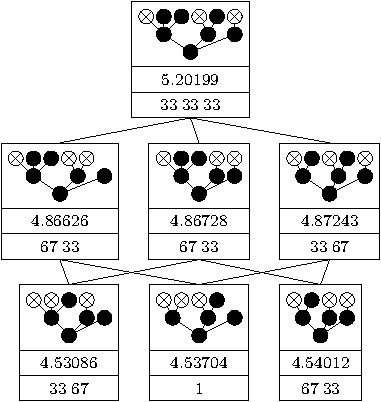
\includegraphics{p3/hlfnfc_not_optimal/000111223_hlfnfc.pdf}
    \caption{HLF schedule while choosing tasks such that there are as few free paths as possible -- overall run time of 5.20199.}
  \end{subfigure}
  \quad
  \begin{subfigure}{.45\textwidth}
    \centering
    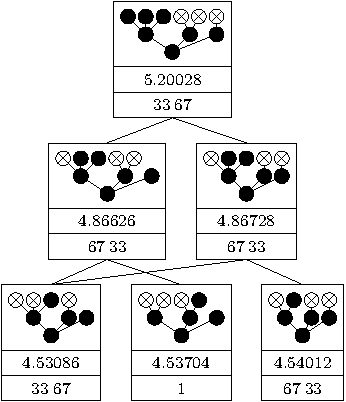
\includegraphics{p3/hlfnfc_not_optimal/000111223_opt.pdf}
    \caption{Optimal schedule (run time 5.20028) has three free paths at the beginning.}
  \end{subfigure}
  \caption{HLF with no free paths is not necessarily optimal.}
  \label{fig:hlfnfc-is-not-optimal}
\end{figure}

\section{Size of the snapshot DAG}
\label{sec:p3-size-of-snapshot-dag-first-attempts}

Similar to the reasoning in section \ref{sec:p2-snapshot-dag}, we can research the size of a snapshot DAG for the P3 case. 
We conducted an experiment and examined the size for snapshot DAGs of intrees containing up to 17 tasks. 
Therefore, we generated all intrees (up to isomorphism) with a certain number of tasks (see section \ref{sec:enumerating-all-intrees} for an algorithm).
Then we computed the following for each intree:
\begin{itemize}
\item Number of distinct (i.e. non-isomorphic) subtrees.
\item Number of snapshots that can be constructed using the LEAF scheduling strategy (i.e. ``try-everything'' scheduling).
\item The size of the \emph{optimal} snapshot DAG.
\end{itemize}

We do so because of the following: It is easily possible to construct an optimal schedule if we take the possible snapshot DAGs of the LEAF scheduler and only leave the choices that yield the best expected run time.

Since the size of the snapshot DAG for an intree with $n$ tasks is at most $n^3$ times as large as the number of subtrees of the original intree, we also computed the number of subtrees for each of these intrees.
That is, we can compare the number of intrees to the number of snapshots to be considered.

The results are summed up in table \ref{tab:num-subtrees-size-of-dags}\todo{Complete!}.

\begin{table}[ht]
  \centering
  \begin{tabular}[ht]{ccccccc}
    \multirow{2}{*}{Tasks} & \multicolumn{2}{c}{Subtrees} & \multicolumn{2}{c}{Snapshots} & \multicolumn{2}{c}{``Optimal DAG''} \\
    & Max & Avg & Max & Avg & Max & Avg \\
    \hline
    3 & 3 & 3.00 & 3 & 3.00 & 3 & 3.00  \\
    4 & 5 & 4.25 & 5 & 4.25 & 5 & 4.25  \\
    5 & 7 & 5.89 & 7 & 5.89 & 7 & 5.89  \\
    6 & 11 & 8.10 & 11 & 8.25 & 11 & 8.05  \\
    7 & 16 & 11.04 & 19 & 11.75 & 16 & 10.81  \\
    8 & 24 &  15.10 & 34 & 17.39 & 22 & 14.37  \\
    9 & 34 &  20.57 & 63 & 26.53 & 31 & 18.76  \\
    10 & 54 &  28.08 & 119 & 41.85 & 41 & 24.16  \\
    11 & 79 &  38.33 & 230 & 67.48 & 55 & 30.67  \\
    12 & 119 & 52.41 & 437 & 112.68 & 71 & 38.41  \\
    13 & 169 &  71.69 & 812 & 184.95 & 89 & 47.49  \\
    14 & 269 &  98.19 & 1510 & 304.41 & 113 & 58.05  \\
    % 15 & 357 &  125.70 & 142 & 67.83  \\
    % 16 & 594 &  171.29 & 184 & 80.55  \\
    % 17 & 850 &  240.39 & 235 & 96.67  \\
  \end{tabular}
  \caption{Number of subtrees, size of the optimized snapshot DAG depending on the number of tasks. ``Subtrees'' denotes the number of distinct subtrees. ``Snapshots'' shows the number of distinct snapshots that have to be examined if we try all possible schedules. The column ``Optimal DAG'' shows the size of the snapshot DAG describing the optimal schedule.}
  \label{tab:num-subtrees-size-of-dags}
\end{table}

As we can see in table \ref{tab:num-subtrees-size-of-dags}, the number of subtrees is (at least for $n\geq  9$) significantly larger than the number of snapshots in the snapshot DAG describing an optimal schedule.

Another interesting fact is that there is no ``strict correlation'' between the number of subtrees and the number of snapshots in the optimal snapshot DAG. That is, there are certain DAGs that have more non-isomorphic subtrees than another DAG, yet -- on the other hand -- more snapshots in the optimal snapshot DAG. As an example, consider the intrees $T_1$ described by 00011111 and $T_2$ described by 00001234: $T_1$ has 19 subtrees and its optimal snapshot DAG contains 13 snapshots, while $T_2$ has only 15 subtrees, but an optimal snapshot DAG containing 14 snapshots.

Moreover, intrees containing $n$ tasks and having the maximal number of subtrees are (at least for $8\leq n \leq 17$) are not the ones having the largest optimal snapshot DAG.

To determine the maximum size of the optimal snapshot DAG for the P3 case, it might be useful to investigate whether the trees that have a large snapshot DAG can be constructed according to a specific pattern. The intrees resulting in snapshot DAGs of maximum size are depicted in figure \ref{fig:intrees-maximum-snapshot-dag-size-p3}. The intrees in this figure seem to behave quite chaotic and we were not able to deduce any pattern according to which they could be generated for general $n$.

\begin{figure}[t]
  \centering
  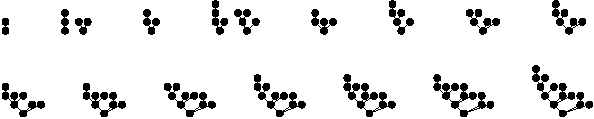
\includegraphics[scale=1.4]{p3/max_unoptimized.pdf}
  \caption{These are the intrees for which the a brute-force algorithm has to generate maximally many snapshots to generate the optimal schedule (maximal compared to all other intrees with the same number $n$ of vertices). We show $2\leq n \leq 14$.}
  \label{fig:intrees-maximum-unoptimized-p3}
\end{figure}

\begin{figure}[t]
  \centering
  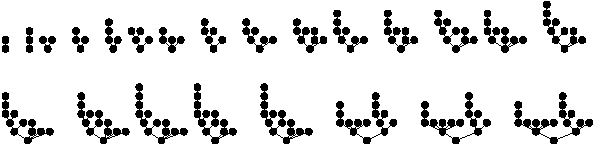
\includegraphics[scale=1.4]{p3/max_snapshot_dag.pdf}
  \caption{These intrees result in \emph{optimal} snapshot DAGs that are larger than all other optimal snapshot DAGs resulting from intrees having the same number of tasks $n$ ($2 \leq n \leq 17$ shown). There seems to be no simple pattern according to which these trees are constructed.}
  \label{fig:intrees-maximum-snapshot-dag-size-p3}
\end{figure}

% \section{Special classes of intrees}
% \label{sec:p3-dag-size-special-class-of-intrees}

% If we consider trees. whose sequence description is of the form $(0, 0, 1, 1, 3, 3, 5, 5, 7,7, 9,9,\dots)$, that have an even number of nodes, then the optimal snapshot DAGs have $\binom{n}{1}+\binom{n}{2}+\binom{n}{3}$ snapshots. \todo{Make this conjecture and nice!}

% \begin{table}[ht]
%   \centering
%   \begin{tabular}{lcc}
%     Class & No. snaps & Opt. size \\
%     $(0,0,1,1,3,3,5,5,\dots)$ & & $\binom{n/2}{1}+\binom{n/2}{2}+\binom{n/2}{3}$ \\
%     $(0,0,0,1,1,1,4,4,4,7,7,7,\dots)$ & & $((n/3)^3 + 2*(n/3))/3$
%   \end{tabular}
%   \caption{Classes and their DAG sizes}
%   \label{tab:special-classes-dag-sizes}
% \end{table}

\section{Degenerate intrees}
\label{sec:p3-degenerate-intrees}

\todo{Definitions: intree, level, suc, adding tasks to trees etc.}

We now focus one one particular class on intrees, namely \emph{degenerate intrees}. A degenerate intree is an intree that consists of one longest chain from the bottom to one leaf, and all other tasks are direct predecessors to one of the tasks within this longest chain.\todo{Figure zeigen.}

\subsection{Intro: Degenerate binary trees}
\label{sec:p3-degenerate-trees-binary}

We researched degenerate binary trees, i.e. trees whose sequence has the structure
\begin{equation*}
  \left( 0,0,a_0,a_1,a_2,a_3,a_4,\dots,a_n \right),
\end{equation*}
for $n$ the total number of tasks within the intree. The values $a_i$ can be recursively defined as follows:
\todo{Sequence-Notation einführen}
\begin{equation*}
  a_k =
  \begin{cases}
    1, & \text{if } k\leq 1 \\
    a_{k-1}, & \text{if } k>1 \text{ is odd} \\
    a_{k-1}+2, & \text{if } k>1 \text{ is even}
  \end{cases}
\end{equation*}

That is, degenerate binary trees have sequences of the form $(0,0,1,1,3,3,5,5,7,7,9,\dots)$.

We now examine how many snapshots are considered if we compute the optimal P3 schedule by considering \emph{all} possibilities and afterwards discarding the bad ones. The results are summed up in table \ref{tab:p3-degenerate-binary-trees-no-snapshots}. We clearly observe that the number of snapshots grows exponentially (at least within the range for $n$ under consideration). A simple pattern that can be observed from table \ref{tab:p3-degenerate-binary-trees-no-snapshots} is that (at least for $n\leq 26$) that the number of snapshots for a degenerate binary tree with $n$ tasks is greater than twice the number of snapshots for a degenerate binary tree with $n-2$ tasks. If $S(n)$ denotes the number of snapshots for a degenerate binary tree, we can formulate $S(n)>S(n-2)$, which we can (by induction) convert to $S(n) > \sqrt 2 ^ n$.

This can be illustrated by the fact that degenerate binary intrees are fully determined by their profile (please see section \ref{sec:p2-profiles} for the definition of profiles). A degenerate binary tree has a profile of the form
\begin{equation*}
  \profile{a,2,2,2,2,\dots,2,1},
\end{equation*}
where $a$ is either $1$ or $2$. Assume the length of the profile (i.e. the height of the degenerate binary tree) is exactly $l$. Then, we have $2\cdot(l-2)+1+a = 2l-1+a$ tasks in total. Assume for now that $a=2$ (i.e. we are dealing with a complete degenerate binary tree) and $l>2$.

A subtree of a this degenerate binary intree having height $l'$ has a profile of the form
\begin{equation*}
  \profile{a_0,a_1,a_2,\dots,a_{l'-2},1},
\end{equation*}
where $1\leq a_0\leq a$ and $1\leq a_i \leq 2$ for all $i\in\left\{ 1,2,\dots,l-2 \right\}$. Using basic combinatorics, we can tell that there must be
\begin{equation*}
  \sum_{l'=0}^{l-1} 2^{l'} = 2^{l} -1
\end{equation*}
distinct subtrees if $a=2$ for profile length (resp. intree depth) $l$.

If $a=1$ and we have a profile length of $l$, we cann argue that there must be as many subtrees as for the profile without the first item (then of length $l-1$) plus the number of profiles of length exactly $l-1$ with one additional 1 prepended. These are exactly $2^{l-2}$.

This, in total leads to our desired bound for $S(n)$.\todo{Genauer machen.}

\begin{table}[t]
  \centering
  \begin{tabular}[ht]{ccc}
    \multirow{2}{*}{Tasks} & \multicolumn{2}{c}{Snapshots} \\
    & Overall & HLF \\
    \hline
    3  &  3       & 3   \\
    4  &  5       & 5   \\
    5  &  7       & 7   \\
    6  &  11      & 11  \\
    7  &  17      & 14  \\
    8  &  28      & 21  \\
    9  &  48      & 25  \\
    10 &  85      & 36  \\
  \end{tabular}
  \begin{tabular}[ht]{ccc}
    \multirow{2}{*}{Tasks} & \multicolumn{2}{c}{Snapshots} \\
    & Overall & HLF \\
    \hline
    11 &  150     & 41  \\
    12 &  276     & 57  \\
    13 &  477     & 63  \\
    14 &  884     & 85  \\
    15 &  1477    & 92  \\
    16 &  2717    & 121 \\
    17 &  4398    & 129 \\
    18 &  7991    & 166 \\
  \end{tabular}
  \begin{tabular}[ht]{ccc}
    \multirow{2}{*}{Tasks} & \multicolumn{2}{c}{Snapshots} \\
    & Overall & HLF \\
    \hline
    19 &  12600   & 175 \\
    20 &  22594   & 221 \\
    21 &  34883   & 231 \\
    22 &  61774   & 287 \\
    23 &  93775   & 298 \\
    24 &  164187  & 365 \\
    25 &  245852  & 377 \\
    26 &  426089  & 456 \\
  \end{tabular}
  \caption{Number of snapshots for degenerate binary trees in the P3 case. The first column depending on the number of tasks. ``Overall'' denotes the number of distinct snapshots that are explored if all possible schedulings are tried. ``HLF'' denotes the number of distinct snapshots for HLF.}
  \label{tab:p3-degenerate-binary-trees-no-snapshots}
\end{table}

Interestingly, degenerate binary intrees, while having a possibly huge amount of snapshots, are probably optimally scheduled by HLF. You can compare the number of HLF snapshots to the number of overal snapshots by looking at table \ref{tab:p3-degenerate-binary-trees-no-snapshots}.

We generalize this fact in the next section.

\subsection{HLF is optimal for degenerate intrees}
\label{sec:p3-degenerate-intrees-hlf-optimal}

\begin{lemma}
  \label{lem:p3-adding-tasks-level-keep-scheduled-same-inequality}
  Let $I$ be a degenerate intree and $x, y$ two (not necessarily distinct) ready tasks within this intree. Let $z_1, z_2$ be two new tasks that will be added to this intree with $level(z_1) > level(z_2)$ in a manner such that $I_1:=I\cup\left\{ z_1 \right\}$ and $I_2:=I\cup\left\{ z_2 \right\}$ are still degenerate intrees. Moreover, the tasks $z_1$ and $z_2$ shall be added in such a way that neither $x$ nor $y$ is a successor of $z_1$ resp. $z_2$ (i.e. $x,y$ stay ready in $I_1$ resp. $I_2$). 
  
  By $T^*_{t_1,t_2,t_3}(I)$ we denote the optimal expected run time that can be acchieved if we \emph{initially} schedule all tasks from the set $\left\{ t_1,t_2,t_3 \right\}$. \todo{Notation auslagern.} Note that this notation does not necessarily require that we actually have three tasks (e.g. if $t_1=t_2$).
  
  Then, if $x,y$ and $z_1$ resp. $z_2$ are used as initial tasks, we have the following for the best acchievable expected run times (for respective initial tasks):
  \begin{equation}
    \label{eq:lemma-p3-adding-tasks-level-keep-scheduled-same-inequality}
    T^{*}_{x,y,z_1}\left(I\cup\left\{ z_1 \right\}\right) > T^{*}_{x,y,z_2}\left( I\cup\left\{ z_2 \right\} \right)
  \end{equation}
\end{lemma}

\begin{proof}
  We prove the claim by induction on the number of nodes:
  
  The induction basis is the case where we have degenerate intrees with 3 tasks\footnote{We start by 3 tasks since these trees are the only ones that allow adding $z_1$ and $z_2$ at different levels such that both $x$ and $y$ stay ready. For an intree with two tasks, the claim can be seen by simply examining that $T(0,0)<T(0,1)$\todo{Improve this footnote.}.} (all of them are depicted in figure \ref{fig:p3-lemma-adding-intrees-induction-start} (only the black nodes)).
  
  \begin{figure}[t]
    \centering
    \begin{tikzpicture}[scale=0.25]
      \newcommand{\treeone}{
        \fill(0,0) circle (0.4);
        \fill(0,1) circle (0.4);
        \fill(0,2) circle (0.4);
        \draw(0,0) -- (0,1);
        \draw(0,1) -- (0,2);
      }
      \newcommand{\treetwo}{
        \fill(0,0) circle (0.4);
        \fill(-.50,1) circle (0.4);
        \fill(.50,1) circle (0.4);
        \draw(0,0) -- (0.5,1);
        \draw(0,0) -- (-.5,1);
      }
      \newcommand{\treethree}{
        \fill(0,0) circle (0.4);
        \fill(0,1) circle (0.4);
        \draw(0,0) -- (0,1);
      }
      % \begin{scope}
      %   \treeone;
      % \end{scope}
      % \begin{scope}[xshift=9cm]
      %   \treetwo;
      % \end{scope}

      \begin{scope}[yshift=-5cm, xshift=-20.5cm]
        \begin{scope}
          \treethree;
          \draw(0,1) -- (0,2);
          \draw[fill=white](0,2) circle (0.4);
          \node at (0,-2) {3};
        \end{scope}
        \node at (2.5,-2) {$>$};
        \begin{scope}[xshift=5cm]
          \treethree;
          \draw(0,0) -- (1,1);
          \draw[fill=white](1,1) circle (0.4);
          \node at (0,-2) {2.5};
        \end{scope}
      \end{scope}

      \begin{scope}[yshift=-5cm, xshift=-3.5cm]
        \begin{scope}
          \treeone;
          \draw(0,2) -- (0,3);
          \draw[fill=white](0,3) circle (0.4);
          \node at (0,-2) {4};
        \end{scope}
        \node at (2.5,-2) {$>$};
        \begin{scope}[xshift=5cm]
          \treeone;
          \draw(0,1) -- (1,2);
          \draw[fill=white](1,2) circle (0.4);
          \node at (0,-2) {3.5};
        \end{scope}
        \node at (8,-2) {$>$};
        \begin{scope}[xshift=11cm]
          \treeone;
          \draw(0,0) -- (1,1);
          \draw[fill=white](1,1) circle (0.4);
          \node at (0,-2) {3.25};
        \end{scope}
        % \node at (4,-1.5) {$4 > 3.5 > 3.25$};
      \end{scope}

      \begin{scope}[yshift=-5cm, xshift=20cm]
        \begin{scope}[xshift=0cm]
          \treetwo;
          \draw(-.5,1) -- (-.5,2);
          \draw[fill=white](-.5,2) circle (0.4);
          \node at (0,-2) {3.25};
        \end{scope}
        \node at (2.5,-2) {$>$};
        \begin{scope}[xshift=5cm]
          \treetwo;
          \draw(0,0) -- (1.5,1);
          \draw[fill=white](1.5,1) circle (0.4);
          \node at (0,-2) {2.83};
        \end{scope}
      \end{scope}
      
    \end{tikzpicture}
    \caption{Adding new tasks to degenerate intrees with less than four nodes such that the resulting intrees are still degenerate. The original (2- resp. 3-node) intrees are drawn black, the newly added tasks are drawn white. Below each intree, we see the corresponding optimal expected run time. The lower the level of the newly added task, the lower the expected run time. This serves as basis for the induction proof for lemma \ref{lem:p3-adding-tasks-level-keep-scheduled-same-inequality}.}
    \label{fig:p3-lemma-adding-intrees-induction-start}
  \end{figure}

  If we add two tasks $z_1$ and $z_2$ with $level(z_1)>level(z_2)$ in a way such that the original ready tasks stay ready and the resulting intrees stay degenerate, we obtain the intrees depicted in figure \ref{fig:p3-lemma-adding-intrees-induction-start} (trees \emph{including} the white nodes). By simply computing the expected optimal run times, we can confirm our claim for intrees with 3 nodes.

  We now do the induction step by considering an intree with $n$ tasks. 
  Let $x,y$ be ready tasks and $z_1$ and $z_2$ to be added with $level(z_1) > level(z_2)$ such that the resulting intrees are degenerate.
  We can now compare the two runs that can occur if $x,y,z_1$ resp. $x,y,z_2$ are initially scheduled. 
  Therefore, we consider what happens in $I_1$ resp. $I_2$ if either $x$, $y$ or $z_1/z_2$ finishes first:

  \begin{itemize}
  \item If $z_1$ resp. $z_2$ is the first task to finish, the resulting intree is exactly $I$. Thus, the remaining run times for these cases are identical if the next task chosen is the same in both trees. We denote the task that may be chosen additionally to $x$ and $y$ by $z'$. If it is the case that only $x$ and $y$ can be scheduled, we set $z'=x$ to simplify notation. The corresponding run time for the resulting intree is then $T^*_{x,y,z'}$

  \item If $x$ is the first task to finish, then the resulting intrees are 
    \begin{equation*}
      I^x_{1}=I_1\setminus\left\{ x \right\} \quad \text{ resp. } \quad I^x_{2}=I_2\setminus\left\{ x \right\}.
    \end{equation*}

    By $x'$ we denote the task that is scheduled next in the optimal schedule for intree $I_1^x$. 
    If there are only two ready tasks left in $I_1^x$ (which then must be $y$ and $z_1$), we set $x'=y$. The expected optimal runtime for $I_1^x$ in this situaion is then given by $T_{x',y,z_1}^*(I_1^x)$.

    We now examine whether $x'$ is also ready in the intree $I_2$:
    \begin{itemize}
    \item If $x'$ is the direct successor of $x$, then $x$ must have been the \emph{single topmost task} and the \emph{single predecessor} of $x'$ (since $I_1^x$ is a degenerate tree). However, since we assumed that $level(z_2)<level(z_1)$ and $z_1$ can not be a predecessor of $x'$ (since $x'$ is ready in $I_1$), it can not be the case that $z_2$ blocks $x'$ in $I_2^x$.

      % Moreover, since $x'$ is ready in $I_1^x$, the task $z_1$ can not be a predecessor of $x'$. Since $level(z_2)<level(z_1)$ and since $I_1^x$ and $I_2^x$ are both degenerate intrees, $z_2$ can not block $x'$.\todo{Genauer ausführen. Evtl. auslagern.}
    \item If $x'$ is not the direct successor of $x$, we recognize the fact that $x'$ must reside on a certain level with in the degenerate intree. 

      If $x'$ is \emph{not} in the topmost level, it can not be blocked by $z_2$ because we assumed that $z_2$ is added in a way such that $I\sup\{z_2\}$ is still a degenerate intree.

      Otherwise (if $x'$ is a topmost task \todo{topmost definieren!}), we still have two subcases:
      \begin{itemize}
      \item If there are other tasks at the same level as $x'$ (i.e. at the topmost level), then we can -- without loss of generality\footnote{Because of isomorphism.} -- assume that $z_2$ was added to another task on the same level as $x'$.
      \item If $x'$ was the \emph{only} topmost task, then it \emph{might} be the case that $z_2$ was chosen in a way such that it is the direct predecessor of $x'$. In this case, we can argue that $level(z_1) > level(z_2)$ and, thus, know that $z_2$ can not block $x'$, because $x'$ is a topmost task.
      \end{itemize}

$x'$ must be on a lower level then $x$ (because we are dealing with a degenerate intree). We assumed that we added $z_2$ in a manner such that $I_2=I\cup\left\{ z_2 \right\}$ is a degenerate subtree. Thus, $z_2$ could not have been added with $x'$ as its successor. Thus, $x'$ is not blocked by $z_2$ in $I_2$.
    \end{itemize}
    We observed that for $I_2^x$, the task $x'$ must be ready.
    
    The intrees $I^x_{1}$ and $I^x_{2}$ have exactly $n$ tasks -- and they have a common subtree, namely
    \begin{equation*}
      I^x := I^x_{1}\setminus\left\{ z_1 \right\}=I^x_{2}\setminus\left\{ z_2 \right\}.
    \end{equation*}

    
    We can now apply the induction hypothesis for the intree $I^x$, since this intree contains only $n-1$ tasks: We have an intree with $n-1$ tasks (namely $I^x$) and two tasks $z_1$ and $z_2$ with $level(z_1)>level(z_2)$, $I^x_1 = I^x\cup\left\{ z_1 \right\}$ and $I^x_2 = I^x\cup\left\{ z_2 \right\}$, implying that $T^*_{x',y,z_1}(I^x_1)>T^*_{x',y,z_2}(I^x_{2})$.
  \item If $y$ is the first task to finish, we argue similar to the $x$ case, thereby considering $I^y_{1},I^y_{2}$ and $I^y$ which are all defined analogously. This finally yields the following inequality: $T^*_{x,y',z_1}(I^y_{1}) > T^*_{x,y',z_2}(I^y_{2})$.
  \end{itemize}

  \todo{Fall für $x=y$ abdecken!}

  The above considerations are illustrated in figure 
\ref{fig:p3-adding-tasks-level-keep-scheduled-same-inequality}.\todo{Figure anpassen!}
  
  \begin{figure}[t]
    \centering
    \newcommand{\drawx}{
      \node[draw=black,circle] at (.9,3) {$x$};
    }
    \newcommand{\drawxx}{
      \node[draw=black,circle] at (.7,2) {$x'$};
    }
    \newcommand{\drawy}{
      \node[draw=black,circle] at (-1.5,4) {$y$};
    }
    \newcommand{\drawyy}{
      \node[draw=black,circle] at (-1.5,3) {$y'$};
    }
    \newcommand{\rawtriangle}{
      \draw
      [dotted, very thick,
      %fill=white!90!black, 
      rounded corners]
      (0,0) -- (3,2) -- (3.5,8) -- (-3.5,8) -- (-3,2) -- cycle;
    }
    \newcommand{\treetriangle}{
      \rawtriangle;
      \drawx;
      \drawy;
    }
    \newcommand{\abstand}{7.5cm}
    \begin{tikzpicture}[scale=.4]
      \begin{scope}[xshift=-\abstand]
        \treetriangle
        \node[draw=black,circle] at (0,6.5) {$z_1$};
      \end{scope}
      \begin{scope}[xshift=\abstand]
        \treetriangle
        \node[draw=black,circle] at (1,5) {$z_2$};
      \end{scope}
      
      \begin{scope}[xshift=-2*\abstand, yshift=-9cm]
        \rawtriangle
        \node[draw=black,circle] at (0,6.5) {$z_1$};
        \drawxx;
        \drawy;
      \end{scope}

      \begin{scope}[xshift=-\abstand, yshift=-9cm]
        \rawtriangle
        \node[draw=black,circle] at (0,6.5) {$z_1$};
        \drawx;
        \drawyy;
      \end{scope}

      \begin{scope}[xshift=0, yshift=-9cm]
        \treetriangle
        \node[draw=black,circle] at (.3,5.5) {$z'$};
      \end{scope}
      
      \begin{scope}[xshift=\abstand, yshift=-9cm]
        \rawtriangle
        \node[draw=black,circle] at (1,5) {$z_2$};
        \drawxx;
        \drawy;
      \end{scope}

      \begin{scope}[xshift=2*\abstand, yshift=-9cm]
        \rawtriangle
        \node[draw=black,circle] at (1,5) {$z_2$};
        \drawx;
        \drawyy;
      \end{scope}
      
      \draw[thick,->](-\abstand,0) -- +(0,-.8);
      \draw[thick,->](-\abstand-2cm,1) -- +(-\abstand+4cm,-1.6);
      \draw[thick,->](-\abstand+2cm,1) -- +(\abstand-4cm,-1.6);

      \begin{scope}[xshift=2*\abstand]
        \draw[thick,->](-\abstand,0) -- +(0,-.8);
        \draw[thick,->](-\abstand-2cm,1) -- +(-\abstand+4cm,-1.6);
        \draw[thick,->](-\abstand+2cm,1) -- +(\abstand-4cm,-1.6);
      \end{scope}
      
      % legend      
      \draw[decoration=brace,decorate=true](-11,8.25) --node[above]{$I_1$} +(7,0);
      \draw[decoration=brace,decorate=true](  4,8.25) --node[above]{$I_2$} +(7,0);
      \draw[decoration={brace,mirror},decorate=true](  -18,-9.5) --node[below, yshift=-.2cm]{$I^x_{1}$} +(6,0);
      \draw[decoration={brace,mirror},decorate=true](-10.5,-9.5) --node[below, yshift=-.2cm]{$I^y_{1}$} +(6,0);
      \draw[decoration={brace,mirror},decorate=true](   -3,-9.5) --node[below, yshift=-.2cm]{$I$} +(6,0);
      \draw[decoration={brace,mirror},decorate=true](  4.5,-9.5) --node[below, yshift=-.2cm]{$I^x_{2}$} +(6,0);
      \draw[decoration={brace,mirror},decorate=true](   12,-9.5) --node[below, yshift=-.2cm]{$I^y_{2}$} +(6,0);
    \end{tikzpicture}

    \caption{Proof sketch for lemma \ref{lem:p3-adding-tasks-level-keep-scheduled-same-inequality}. By induction hypothesis, we have that $T^*_{x',y,z_1}(I^x_{1}) > T^*_{x',y,z_2}(I^x_{2})$ and $T^*_{x,y',z_1}(I^y_{1}) > T^*_{x,y',z_2}(I^y_{2})$, from which we deduce $T^*_{x,y,z_1}(I_1) > T^*_{x,y,z_2}(I_2)$. Note that $z_2$ can not block $x'$ or $y'$ since $z_1$ didn't block any of the two and we required that adding $z_1$ resp. $z_2$ still results a degenerate tree.}
    \label{fig:p3-adding-tasks-level-keep-scheduled-same-inequality}
  \end{figure}
  
  Now we argue that the run times for $I_1$ and $I_2$ can be computed as follows:
  \begin{align*}
    T^*_{x,y,z_1}(I_1) & = 
      \frac{1}{3} + 
      \frac{1}{3}\cdot \left( 
        T_{x,y,z'}^*(I) + 
        T^*_{x',y,z_1}(I^x_{1}) +
        T^*_{x,y',z_1}(I^y_{1}) 
      \right)
      \\
    T^*_{x,y,z_2}(I_2) & = 
      \frac{1}{3} + 
      \frac{1}{3}\cdot \left( 
        T_{x,y,z'}^*(I) + 
        T^*_{x',y,z_2}(I^x_{2}) +
        T^*_{x,y',z_2}(I^y_{2}) 
      \right)
  \end{align*}

  We will now use the aforementioned inequalities $T^*_{x',y,z_1}(I^x_{1}) > T^*_{x',y,z_2}(I^x_{2})$ and $T^*_{x,y',z_1}(I^y_{1}) > T^*_{x,y',z_2}(I^y_{2})$:
\begin{align*}
    T^*_{x,y,z_1}(I_1) & = 
      \frac{1}{3} + 
      \frac{1}{3}\cdot \left( 
        T_{x,y,z'}^*(I) + 
        T^*_{x',y,z_1}(I^x_{1}) +
        T^*_{x,y',z_1}(I^y_{1}) 
      \right)
      > 
      \\
      & >
      \frac{1}{3} + 
      \frac{1}{3}\cdot \left( 
        T_{x,y,z'}^*(I) + 
        T^*_{x',y,z_2}(I^x_{2}) +
        T^*_{x,y',z_2}(I^y_{2}) 
      \right) 
      = T^*_{x,y,z_2}(I_2).
  \end{align*}

  This proves our claim.    
\end{proof}

\paragraph{Application of lemma \ref{lem:p3-adding-tasks-level-keep-scheduled-same-inequality}}

We presented lemma \ref{lem:p3-adding-tasks-level-keep-scheduled-same-inequality} in a way that involved adding tasks to a certain intree, because this related well to our proof technique. In practice, we can use it to compare two degenerate intrees with $n$ nodes and that have a common subtree containing $n-1$ nodes.

We can now derive the following theorem.

\begin{theorem}
  Degenerate intrees are optimally scheduled by HLF.
\end{theorem}

\begin{proof}
  Consider a degenerate intree with $n=3$ tasks. It is trivially clear that for P3, a HLF schedule is optimal for this intree (see figure \ref{fig:p3-lemma-adding-intrees-induction-start} to see what these intrees look like).
  
  Consider now a degenerate tree $I$ with $n$ nodes and assume that we know that for all degenerate trees with $n-1$ nodes HLF is optimal for three processors. If $I$ has two or less topmost tasks, it is obvious that we have to use HLF (since we can use at most two processors and HLF is known to be optimal for two processors \todo{Referenz und Beweis in P2-Kapitel}).

  Thus, we only have to focus on the case where $I$ has at laast three ready tasks.

  If we choose three topmost tasks $x,y,z$ of $I$, we can argue as follows: If $x$ is the task that finishes first, for the resulting subtree $I\setminus \left\{ x \right\}$, we can be sure that we can choose the next task such that we adhere to HLF, thus choosing the optimal solution for $I\setminus\left\{ x \right\}$ (by induction hypothesis). The same holds if $y$ or $z$ finishes first.
  
  We now consider a \todo{(possibly?) }non-HLF schedule for $I$ and compare it to the HLF schedule described before.
  Let $x',y',z'$ be the tasks to be chosen such that at least $x\neq x'$ or $y\neq y'$ or $z\neq z'$. We can -- without loss of generality -- assume $level(x')\leq level(x)$, $level(y')\leq level(y')$, $level(z')\leq level(z)$. If $x'$ is the first task to finish, we consider the degenerate intree $I\setminus\left\{ x' \right\}$. Since $I \setminus \left\{ x' \right\}$ is a degenerate intree with $n-1$ tasks, it would be optimal to use HLF. However, using HLF may or may not be possible depending on our previous choices of $y'$ and $z'$. That is, the optimum for $I\setminus\left\{ x' \right\}$ \emph{might} be acchieved if we chose $y'$ and $z'$ accordingly. From this we can conclude that the optimal expected run time is at least $T_{HLF}\left( I\setminus\left\{ x' \right\} \right)$, where $T_{HLF}$ denotes the run time for HLF (which we know, by induction, is optimal).

  Now we compare the run time for $I\setminus\left\{ x' \right\}$ to the optimal run time for $I \setminus\left\{ x \right\}$, which is exactly given by $T_{HLF}\left( I \setminus\left\{ x \right\} \right)$. We recognize that $I\setminus\left\{ x' \right\}$ and $I\setminus\left\{ x \right\}$ have a common subtree, namely $I\setminus\left\{ x,x' \right\}$ with $n-2$ tasks.
  
  Moreover, we know that for both $I\setminus\left\{ x \right\}$ and $I\setminus\left\{ x' \right\}$ HLF is optimal (because of our induction hypothesis) and that for $I\setminus\left\{ x \right\}$ and $I\setminus\left\{ x' \right\}$ both $y$ and $z$ must be in the optimal (i.e. HLF) schedule since $y$ and $z$ are two of the three topmost tasks. At last, we have $level(x) \geq level(x')$.
  Thus, we can apply lemma \ref{lem:p3-adding-tasks-level-keep-scheduled-same-inequality} for the degenerate tree $I\setminus \{x,x'\}$ with tasks $y$ and $z$ and deduce that
  \begin{equation*}
    T_{x',y,z}(I\setminus\{x\}) 
    \leq 
    \underbrace{T_{x,y,z}(I\setminus\{x'\})}_{\text{Optimal for $I\setminus \{x'\}$}}.
  \end{equation*}
  Equality follows if $x$ and $x'$ are on the same level.

  As stated before, for the intree $I\setminus\{x'\}$, the schedule chosen \emph{might} not be a HLF-one. In this case, the schedule performs even worse than $T_{x,y,z}(I\setminus\{ x'  \})$, since the optimal schedule would choose $x,y,z$ as scheduled tasks. This means that
  \begin{equation*}
    T_{x,y,z}(I\setminus\{x'\})
    \leq
    T_{x'',y',z'}(I\setminus\{x'\}),
  \end{equation*}
  where $x''$ is the task chosen by the non-HLF schedule, finally implying that
  \begin{equation*}
    T_{HLF}(I\setminus\{x\})
    \leq
    T_{x'',y',z'}(I\setminus\{x'\}),
  \end{equation*}
  because the HLF schedule is at least as good as the schedule that starts out with tasks $x',y,z$.
  We argue similar for tasks $y$ and $y'$ resp. $z$ and $z'$ and finally obtain the following:

  \begin{eqnarray*}
    T_{x',y,z}(I\setminus\{x\})
    & \leq &
    T_{x'',y',z'}(I\setminus\{x'\}) \\
    T_{x,y',z}(I\setminus\{y\})
    & \leq &
    T_{x',y'',z'}(I\setminus\{x'\}) \\
    T_{x,y,z'}(I\setminus\{z\})
    & \leq &
    T_{x',y',z''}(I\setminus\{x'\}) \\
  \end{eqnarray*}
  Note that if e.g. $x=x'$, the above three equations are still satisfied.
  Combining the above inequalities yields that
  \begin{eqnarray*}
    %T_{HLF}(I) = 
    T_{x,y,z}(I) 
    & \leq & 
    \frac{1}{3} + \frac{1}{3} \cdot 
    \left( 
      T_{x',y,z}(I\setminus\{x\}) +
      T_{x,y',z}(I\setminus\{y\}) +
      T_{x,y,z'}(I\setminus\{z\})
    \right) 
    \leq \\
    & \leq &
    \frac{1}{3} + \frac{1}{3} \cdot 
    \left( 
      T_{x'',y',z'}(I\setminus\{x'\}) +
      T_{x',y'',z'}(I\setminus\{y'\}) +
      T_{x',y',z''}(I\setminus\{z'\})
    \right) \leq \\
    & \leq &
    T_{x',y',z'}(I)
  \end{eqnarray*}

  This finally shows that a HLF schedule is at least as good as an arbitrary other task, meaning that HLF is optimal for three processors on degenerate trees.
\end{proof}

\section{Parallel chains}
\label{sec:p3-parallel-chains}

We will now consider another class of intrees that can be shown to have HLF as optimal schedules.

\begin{definition}[Parallel chain]
  Let $I$ be an intree. We call $I$ a \emph{parallel chain}, if each task except the root has at most one predecessor. The root may have arbitrarily many predecessors.
\end{definition}

\todo{Figure von einer parallel chain.}

\begin{lemma}
  \label{lem:parallel-chains-chain-switching-higher-is-worse}
  Let $I$ be a parallel chain with three ready tasks $x,y,z$. Such that $level(x)>level(y)$. Let $x'$ resp. $y'$ be two new nodes that are added as predecessors of $x$ resp. $y$. Then, $T_{x',y,z}(I\cup\left\{ x' \right\}) > T_{x,y',z}(I\cup\left\{ y' \right\})$. \todo{T-Notation mit Index mal anständig definieren!}
\end{lemma}

\begin{proof}
  We consider the parallel chain $I\cup\left\{ x' \right\}$ and its optimal schedule. We then construct a schedule for $I\cup\left\{ y' \right\}$ whose run time is less than the optimal run time for $I\cup\left\{ x' \right\}$.
  
  We observe that in $I\cup\left\{ x' \right\}$ either $x'$, $y$ or $z$ finishes first. For each of these cases we now show that we can construct a corresponding schedule in $I\cup\left\{ y' \right\}$ such that the corresponding run time in $I\cup\left\{ y' \right\}$ is at most the one in $I\cup\left\{ x' \right\}$.

  \begin{itemize}
  \item If $x'$ finishes first in $I\cup\left\{ x' \right\}$, then obtain the same intree like if $y'$ finishes first in $I\cup\left\{ y' \right\}$. Thus, we can assume the two resulting schedules to have the same run time.
  \item If $z$ finishes first, we can argue by induction since the trees
    \begin{equation*}
      I\cup\left\{ x' \right\}\setminus\left\{ z \right\}
      \quad
      \text{ and }
      \quad 
      I\cup\left\{ y' \right\}\setminus\left\{ z \right\}
    \end{equation*}
    both have $n-1$ tasks and can be obtained by attaching $x'$ resp. $y'$ to the parallel chain $I\setminus\left\{ z \right\}$. We then know -- by induction -- that $T_{x',y,z}(I\cup\left\{ x' \right\}\setminus\left\{ z \right\}) > T_{x,y',z}(I\cup\left\{ y' \right\}\setminus\left\{ z \right\})$.
  \item It remains to explain what to do if $y$ finishes in $I\cup\left\{ x' \right\}$ compared to if $x$ finishes first in $I\cup\left\{ y' \right\}$.
    
    The two respective intrees then are
    \begin{equation*}
      I\cup\left\{ x' \right\}\setminus\left\{ y \right\} 
      \quad
      \text{ and }
      \quad
      I\cup\left\{ y' \right\}\setminus\left\{ x \right\}.
    \end{equation*}
    
    By induction, we know that
    \begin{equation*}
      T_{x', z}(I\cup\left\{ x' \right\}\setminus\left\{ y \right\})
      >
    \end{equation*}
  \end{itemize}
\end{proof}

\begin{lemma}
  \label{lem:parallel-chains-adding-tasks-level-comparison}
  Let $I$ be a parallel chain and $x, y$ two (not necessarily distinct) redy tasks within $I$. Let $z_1$ and $z_2$ be two new tasks to be added to $I$ with $level(z_1) > level(z_2)$ and $I_1=I\cup\left\{ z_1 \right\}, I_2=I\cup\left\{ z_2 \right\}$.
  
  Then, $T_{x,y,z_1}(I_1) > T_{x,y,z_2}(I_2)$, where $T_{a,b,c}{I}$ denotes the optimal run time that can be acchieved if $a,b,c$ are chosen as initially scheduled tasks.
\end{lemma}

\begin{proof}
  The proof is very similar to the one for lemma \ref{lem:p3-adding-tasks-level-keep-scheduled-same-inequality}. We start by examining small chain trees (with four or less tasks --- see figure \ref{fig:p3-lemma-adding-intrees-induction-start}) and confirm our claim by simply examining the execution times.
  
  We now consider a parallel chain $I$ with $n$ tasks, and tasks $x,y$ and $z_1, z_2$ as specified in the requirements for lemma \ref{lem:parallel-chains-adding-tasks-level-comparison}. We now compare the run times $T_{x,y,z_1}(I_1)$ and $T_{x,y,z_2}(I_2)$, where $I_1=I\cup\left\{ z_1 \right\}$ and $I_2=I\cup\left\{z_2  \right\}$.

  We do a case distinction on which task is to finish first (and compare the situation for $I_1$ and $I_2$):
  \begin{itemize}
  \item If $z_1$ resp. $z_2$ is the first task to finish, we can argue that the run time for the resulting trees can be the same if we choose -- coming from $I_2$ -- the same task that optimally would be chosen coming from $I_1$ (if coming from $I_1$ takes no task at all, we can also do so for $I_2$). 
  \item If $x$ is the first task to finish, we denote by $x'$ the task that would be optimally chosen if we come from $I_1$. We now distinguish:\todo{Was, wenn kein $x'$ gewählt werden kann?}
    \begin{itemize}
    \item If $x'$  is the direct successor of $x$, then $x'$ can only be blocked by $z_2$ if $x'$ is the root. In this case, however, $x'$ would have been blocked by $z_1$ which leads to a contradiction since $x'$ is ready.

      So, we can assume that $x'$ is \emph{not} the root. Thus, we can argue that $x'$ \emph{must} be the end of some chain in $I_1\setminus\left\{ x \right\}$, and can not be blocked by $z_2$. So, $x'$ is ready in $I_2\setminus\left\{ x \right\}$ as well.
    \item If $x'$ is not the direct successor of $x$, then $x'$ can not be the root and $x'$ can be blocked by $z_2$ in $I_2$.
      \begin{itemize}
      \item If $x'$ is \emph{not} blocked by $z_2$, then it is ready in $I_2$.
      \item If $x'$ is exactly the successor of $z_2$, then we 
      \end{itemize}

    \end{itemize}

  \end{itemize}

\end{proof}

\section{Conjectures}
\label{sec:p3-conjectures}

During our research, we recognized some patterns that we are tempted to transform into some conjectures. We were, however, not yet able to prove or disprove them. This section shows the most important ones that could easily be used to decrease the number of snapshots that have to be examined if we want to compute the optimal snapshot by exhaustive search.

\begin{conjecture}
  Parallel chains are optimally scheduled by HLF.
\end{conjecture}

\begin{conjecture}[Very likely]
  For each snapshot resulting from an optimal schedule, at least one top-most task is scheduled.
\end{conjecture}

\begin{conjecture}[Weak one]
  For each snapshot resulting from an optimal schedule, at least two top-most tasks are scheduled.
\end{conjecture}

\begin{conjecture}
  If for an intree only non-top tasks are scheduled, you can exchange one of the non-top tasks with a top-tasks and obtain a better run time.
\end{conjecture}

The main problems we faced when we tried to prove the above conjectures can be summarized as follows:
\begin{itemize}
\item The particular intree structure is not necessarily maintained over the induction step --- and if so, many case distinctions may be required.
\item Comparing different intrees seems to be quite cumbersome, especially if we do not know which tasks are scheduled.
\end{itemize}


%%% Local Variables:
%%% TeX-master: "../thesis.tex"
%%% End: 